\documentclass[10pt,a4paper]{article}
\usepackage[italian]{babel}
\usepackage[T1]{fontenc}
\usepackage[utf8]{inputenc}
\usepackage[affil-it]{authblk}
\usepackage{lineno}
\usepackage{amsmath}
\usepackage{amsfonts}
\usepackage{amssymb}
\usepackage{graphicx}
\usepackage{subcaption}
\usepackage[hidelinks]{hyperref}


\newtheorem{remark}{Osservazione}
\newtheorem{definition}{Definizione}
\newtheorem{theorem}{Teorema}

\newcommand{\ww}{\mathbf{w}}
\newcommand{\vv}{\mathbf{v}}
\newcommand{\ee}{\mathbf{e}}
\newcommand{\ii}{\mathbf{i}}
\newcommand{\oo}{\mathbf{o}}


\begin{document}
\title{Appunti di Artificial Intelligence}

\author{Ivan Masnari%
  \thanks{e-mail: \texttt{ivan.masnari@studenti.unimi.it}}}
\affil{Facoltà di Informatica, UniMi, Milano}

\date{Ultima modifica: \today}
\maketitle

\tableofcontents
\pagebreak
\section{Introduzione}

Dato un qualunque sistema, se disponiamo di un insieme di leggi o regole che lo descrivono completamente (nel caso di un sistema fisico avremmo delle equazioni differenziali) potremmo, in teoria, calcolarne in ogni momento lo stato e, quindi, prevederne l'evoluzione nel tempo. 
Tuttavia, nella vita di ogni giorno capita spesso di non avere a disposizione una conoscenza perfetta di un certo sistema. Tale informazione:
\begin{enumerate}
\item{può mancare.}
\item{possiamo averne una conoscenza approssimata.}
\end{enumerate}
L'intelligenza artificiale nasce con lo scopo di estrarre conoscenza direttamente dai dati in nostro possesso attraverso strumenti automatici. Questo modello si differenzia rispetto alla descrizione \emph{a priori} del sistema, in quanto lo simula per comprenderne \emph{a posteriori} il suo comportamento. Per far questo, è stato utile studiare come gli esseri viventi interagiscano con l'ambiente circostante e come vi si adattino.
Vari modelli di intelligenza artificiale sono stati proposti lungo la storia della disciplina. Una categorizzazione preliminare che si fa in letteratura è quella tra modelli:
\begin{itemize}
\item{\emph{simbolici}, in cui i dati vengono sottoposti a codifica e solo dopo manipolati. Storicamente questo è stato il primo approccio adottato (vedi sistemi esperti degli anni '70).}
\item{\emph{pre-simbolici}, in cui i dati vengono manipolati direttamente, senza la mediazione di una codifica. Fanno parte di questa famiglia: le reti neurali, i sistemi fuzzy e gli algoritmi evolutivi.}
\end{itemize}
Nel corso ci concentreremo sui secondi.

\section{Reti neurali}

\subsection{Background biologico}

Il nostro cervello ci permette di analizzare in maniera molto sofisticata l'ambiente in cui ci troviamo per agire nel miglior modo possibile (esempio: se riconosciamo un leone nella savana, scappiamo nell'altra direzione). Queste analisi sono basate sul funzionamento del cervello: come estrae informazioni, come queste interagiscono con le informazioni contenute in memoria, etc. Lo studio di questi processi è un campo di ricerca molto attivo e multidisciplinare dove convergono gli interessi della biologia, della medicina e della psicologia.
Tali studi ci offrono dei modelli che simulano l'attività celebrale. Proprio questi modelli, vengono poi utilizzati dall'informatica per offrire strumenti di predizione, ottimizzazione e problem-solving in vari campi applicativi (guida automatizzata, smart cities, etc.). Il successo di questi modelli è condizionato dal fatto che il nostro cervello è un potente computer capace di computare in parallelo grandi porzioni di dati. Ma come funziona esattamente?

\begin{figure}
\centering
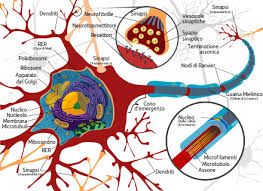
\includegraphics[scale=0.7]{img/neurone.jpeg}
\caption{Neurone}
\label{fig:1}
\end{figure}

Il cervello è composto da miliardi di cellule dette \emph{neuroni} (Figura \ref{fig:1}). Il neurone a sua volta è costituito da:
\begin{itemize}
\item{i \emph{dendriti}, i quali sono filamenti raggiunti dalle terminazioni di altri neuroni e che gli permettono di raccogliere informazioni grazie a processi biochimici originati dai così detti \emph{neurotrasmettitori}.}
\item{l'\emph{assone}: un lungo filamento che parte dal corpo centrale della cellula e trasmette segnali elettrici che, a loro volta, vanno ad attivare altri neuroni attraverso il rilascio di neurotrasmettitori.}
\end{itemize}

Quando e come il neurone trasmetta il segnale di attivazione dipende dal particolare modello fisiologico che si voglia adottare. Solitamente si considera un \emph{threshold}, superato il quale, l'assone viene depolarizzato e la differenza di potenziale provoca il passaggio di una corrente. Un diverso modello prende in considerazione non tanto la potenza dello stimolo quanto il loro numero. 
Questa struttura a network offre ottime prestazioni. Per un confronto con una CPU classica alleghiamo la seguente tabella:

\begin{figure}
\centering
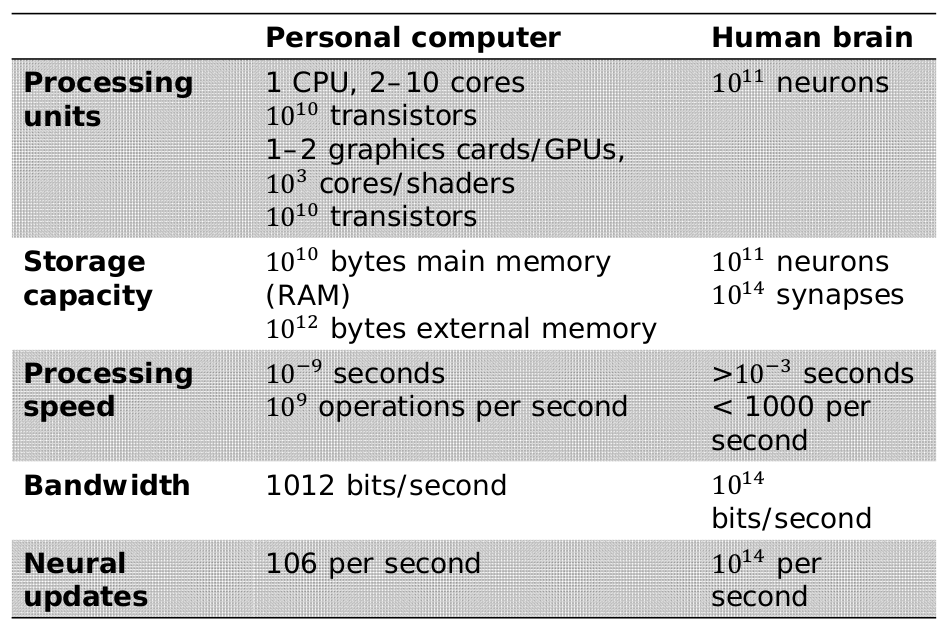
\includegraphics[scale=0.3]{img/cpuvshuman.png}
\end{figure}

\newpage

I vantaggi delle reti neurali sono:

\begin{enumerate}
\item{Alta velocità di calcolo, grazie al parallelismo.}
\item{Tolleranza ai guasti: la rete rimane funzionale anche quando molti neuroni smettono di funzionare.}
\item{La performance degrada in modo lineare con il numero di neuroni danneggiati.}
\item{Ottimo per l'apprendimento induttivo.}
\end{enumerate}

\subsection{Threshold logic unit}

Per implementare una rete neurale artificiale occorre trovare un analogo del neurone naturale. Tale compito è svolto dalle \emph{threshold logic unit}, nel seguito TLU. Una TLU è costituita da $n$ variabili di input $x_1 \dots x_n$ e un output $y$. Ad ogni unità viene assegnato un \emph{threshold} $\theta$ e ad ogni variabile di input un peso $w_i$ dove $i \in \{1, \dots ,n\}$ che rappresenta la rilevanza ai fine della computazione di quel particolare input.
L'output della TLU viene calcolato secondo la seguente formula:

\begin{equation}
y =  \begin{cases}
    1 & \text{se } \sum w_ix_i \geq \theta \\
    0 & \text{altrimenti} 
   \end{cases}
\end{equation}

Attraverso questo semplice meccanismo possiamo simulare alcune funzioni booleane. Se volessimo computare l'AND logico tra due input $x_1$ e $x_2$ basta assegnare valori ai pesi e al threshold in modo che soddisfino il seguente sistema di disequazioni:

\begin{equation}
	\begin{cases}
    w_1 + w_2 \geq \theta \\
    w_1 < \theta\\
    w_2 < \theta
   \end{cases}
\end{equation}

Risulta evidente che l'unica circostanza in cui l'output della TLU verrà posto ad 1 sarà quando entrambi gli input si trovano a 1. Inoltre, si noti che esistono varie scelte possibili di pesi e threshold che verificano le diseguaglianze.

\subsection{Interpretazione geometrica}

La condizione che calcola l'output della TLU somiglia molto da vicino all'equazione di un iperpiano (ovvero, un piano in $n$ dimensioni):

\begin{equation}
	 \sum w_ix_i + \theta = 0 
\end{equation}

Se pensiamo al caso precedente dell'AND logico e consideriamo i valori di input come coordinate in uno spazio bidimensionale, possiamo vedere che la retta definita da $x_1w_1 + x_2w_2 + \theta = 0$ corrisponde al confine che separa quelle combinazioni di valori che restituiscono come output 1 e quelle che, invece, restituiscono 0 (vedi Figura 2). \\
Da quanto detto, tuttavia, si può dedurre che una singola TLU potrà computare solo funzioni \emph{linearmente separabili}, ovvero funzioni in cui le coordinate associate agli input che restituiscono 1 possono essere separate da quelle che restituiscono 0 da una funzione lineare (punto, retta, piano o iperpiano a seconda della dimensione). 

\begin{figure}
\centering
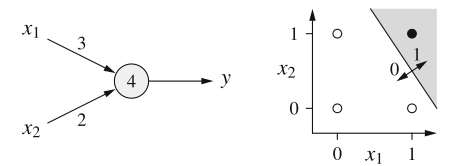
\includegraphics[scale=0.5]{img/geometria.png}
\caption{Rappresentazione geometrica della TLU per $x_1 \land x_2$}
\label{fig:2}
\end{figure}

\begin{definition}
Un insieme di punti $X$ in uno spazio euclideo si dice \emph{convesso} se e solo se non è vuoto, è connesso e ogni coppia di punti può essere congiunta da un segmento.
\end{definition}
\begin{definition}
Un \emph{guscio convesso} di un insieme di punti $X$ in uno spazio euclideo è il più piccolo insieme convesso che contiene $X$.
\end{definition}
\begin{theorem}
Due insiemi di punti $X$ e $Y$ si dicono linearmente separabili se e solo se i loro gusci convessi sono tra loro disgiunti.
\end{theorem}

Questo significa che già all'interno delle funzioni booleane ne esistono alcune che non possono essere simulate da una TLU. Come, per esempio, la doppia implicazione. Sebbene solo due funzioni booleane a due argomenti non siano linearmente indipendenti, al crescere degli argomenti il numero di funzioni che sono linearmente indipendenti diminuisce rapidamente. Per un numeri di argomenti arbitrariamente grande, una singola TLU non può calcolare "quasi" nessuna funzione.

\begin{figure}
\centering
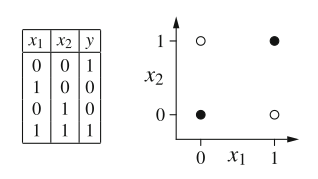
\includegraphics[scale=0.5]{img/doppiaimplicazione.png}
\caption{La doppia implicazione non è linearmente separabile}
\label{fig:3}
\end{figure}

Il problema può essere ovviato attraverso la costruzione di network di TLU più complessi. Come esempio consideriamo il network che simula la doppia implicazione (vedi figura \ref{fig:4}).

\begin{figure}
\centering
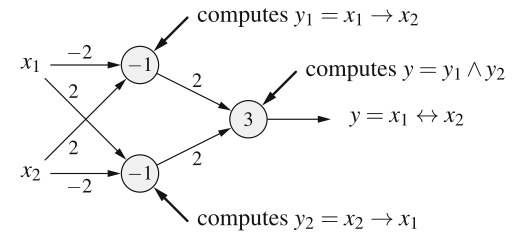
\includegraphics[scale=0.5]{img/netTLU.png}
\caption{network di TLU che simula la doppia implicazione}
\label{fig:4}
\end{figure}

\subsection{Training delle TLU}

L'interpretazione geometrica ci da una intuizione su come costruire una TLU avente 2 o 3 input, ma non è un metodo scalabile, né automatizzato. Come far evolvere una TLU affinché converga in modo autonomo ad una soluzione?
Un algoritmo che ci permette di automatizzare il processo è il seguente:

\begin{enumerate}
\item{Inizializzare i pesi e il threshold con valori randomici.}
\item{Determinare l'errore nell'output per un insieme di controlli. L'errore viene calcolato come una funzione dei pesi e del threshold $e(w_1,\dots,w_n,\theta)$.}
\item{Aggiornare i pesi e il threshold per correggere l'errore.}
\item{Iterare finché l'errore si annulla.}
\end{enumerate}

Mostriamo il comportamento dell'algoritmo nel caso più semplice, in cui abbiamo un threshold ed un unico input (quindi, un unico peso associato). Poniamo che si voglia allenare il nostro neurone a calcolare la negazione booleana. Sia $x$ l'input, $w$ il peso associato e $\theta$ il threshold, allora l'output $y$ sarà definito come:

\begin{equation}
	y = \begin{cases}
    1 & \text{se } 0w = 0 \geq \theta \\
    0 & \text{se } 1w = w \geq \theta
   \end{cases}
\end{equation} 

Calcoliamo la funzione errore al variare di $w$ e $\theta$. Nel caso che $x = 0$ l'errore sarà 0 per un $\theta$ negativo e 1 per un $\theta$ negativo. Il peso non avrà alcuna influenza perché viene annullato nella moltiplicazione con l'input. Quando, invece, $x = 1$, avremo che la funzione dipenderà da entrambi i parametri (vedi Figura \ref{fig:5}).

\begin{figure}
\centering
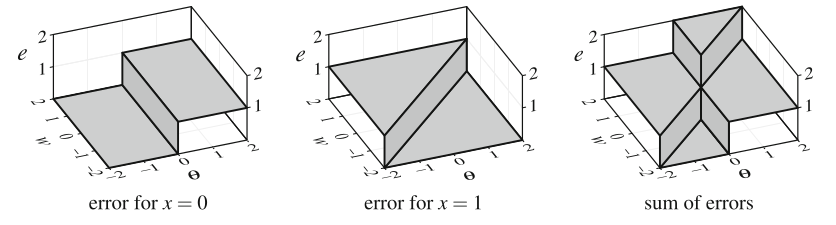
\includegraphics[scale=0.4]{img/error1.png}
\caption{funzione di errore per la negazione booleana}
\label{fig:5}
\end{figure}

La funzione di errore così calcolata non può essere usata direttamente nella nostra computazione perché è composta da plateau e, quindi, non è ovunque derivabile. La soluzione è quella di calcolare la funzione di errore in modo tale che ci offra una misura di "quanto sbagliata" sia la relazione tra pesi e threshold. Otterremo così una funzione di errore che, seppur ancora non differenziabile, (vedi Figura \ref{fig:6}) lo sia localmente nei punti in cui l'errore si discosta da $0$. Ciò che faremo per correggere l'errore, dunque, sarà discendere verso l'area dove la funzione di errore si annulla. Questo è possibile esattamente perché abbiamo costruito una funzione derivabile nei punti in cui ci interessa, e cioè possiamo sempre calcolare la direzione migliore da prendere perché si "scenda".
Ci sono due modi di immaginare il processo di allenamento del neurone:

\begin{itemize}
\item{\emph{Online learning}: dove correggiamo l'errore individualmente per ogni scelta dell'input.}
\item{\emph{Batch learning}: dove prendiamo in considerazione l'errore cumulato su una sequenza di input prima di applicare le correzioni.}
\end{itemize}

\begin{figure}
\centering
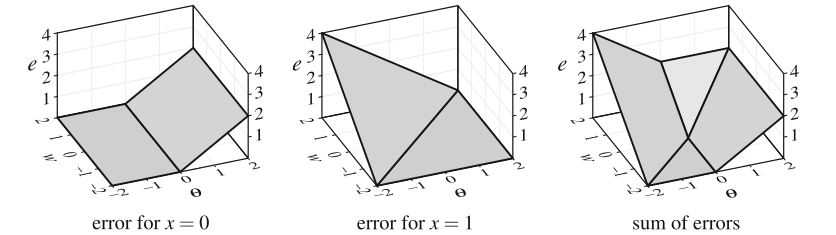
\includegraphics[scale=0.4]{img/error2.png}
\caption{funzione di errore differenziabile}
\label{fig:6}
\end{figure}

Definiamo di seguito la \emph{delta rule} o \emph{procedura di Widrow-Hoff} per allenare le TLU:

\begin{definition}
Sia $\vv$ = ($x_1, \dots, x_n$) il vettore di input di una TLU, \emph{o} l'output aspettato e \emph{y} il valore attuale. Se \emph{o} = \emph{y}, abbiamo finito. Al contrario, per ridurre l'errore computeremo nuovi valori per il threshold e i pesi nel seguente modo:
$$
\theta^{(new)} = \theta^{(old)} + \Delta\theta \text{ con } \Delta\theta = -\eta(\emph{o} - \emph{y})
$$
$$
\forall i \in \{1, \dots, n\}:w_i^{(new)} = w_i^{(old)} + \Delta w_i \text{ con } \Delta w_i = \eta(\emph{o} - \emph{y})x_i
$$
dove $\eta$ è il \emph{learning rate}. Più è alto, più i cambiamenti sui pesi e sui threshold sono drastici.

\end{definition}

Abbiamo visto prima, tuttavia, che non tutte le funzioni possono essere computate. Per le funzioni linearmente separabili esiste un teorema che ci garantisce che applicando la \emph{delta rule} l'algoritmo converga ad una soluzione.

\begin{theorem}
Sia $L = \{(\vv_1,\emph{o}_1), \dots, (\vv_n,\emph{o}_n)\}$ una sequenza di pattern di allenamento per la TLU, dove $\vv_i$ sono i vettori di input e $\emph{o}_i$ l'output atteso. 
Siano inoltre $L_0 = \{(\vv,\emph{o}) \in L | \emph{o} = 0\}$ e $L_1 = \{(\vv,\emph{o}) \in L | \emph{o} = 1\}$ rispettivamente gli insiemi delle coppie di pattern che hanno come output atteso 0 e quelle che hanno come pattern atteso 1. Se $L_0$ e $L_1$ sono linearmente separabili, allora esiste un $\ww$ vettore di pesi e un $\theta$ threshold t.c.:
$$
\forall (\vv,0) \in L_0: \ww\vv < \theta 
$$
$$
\forall (\vv,1) \in L_1: \ww\vv \geq \theta
$$
\end{theorem}

\begin{remark}
Negli esempi precedenti abbiamo codificato il valore booleano \emph{falso} come 0 e \emph{vero} come 1. Questa scelta ha lo svantaggio che, nel caso di \emph{falso}, i pesi corrispondenti non possano essere modificati perché la formula contiene l'input come fattore. Per evitare il problema si ricorre in letteratura ad una diversa codifica chiamata \emph{ADALINE} (ADAptive LINear Element), dove \emph{falso} viene ad assumere il valore $-1$ e il \emph{vero} $1$.
\end{remark}

Notiamo che questa procedura di allenamento vale solo per le singole TLU, ma abbiamo prima visto che le TLU possono computare solo funzioni linearmente separabili. Sebbene questo inconveniente si possa evitare prendendo in esame \emph{network} di TLU, questa procedura non si estende naturalmente a quel caso.

\subsection{Artificial neural network}

Un artificial neural network (in quello che segue ANN) può essere rappresentata come un grafo diretto $G = (U,C)$ dove i nodi sono TLU e gli archi sono le connessioni tra le varie unità. L'insieme dei nodi $U$ può essere partizionato in tre sottoinsiemi:

\begin{itemize}
\item{$U_{(in)}$: è l'insieme dei nodi di input, i quali ricevono in modo diretto l'informazione dall'ambiente.}
\item{$U_{(out)}$: è l'insieme dei nodi di output, i quali sono i soli nodi a comunicare con l'esterno.}
\item{$U_{(hidden)}$: è l'insieme dei nodi interni, i quali propagano la computazione.}
\end{itemize}

\begin{figure}
\centering
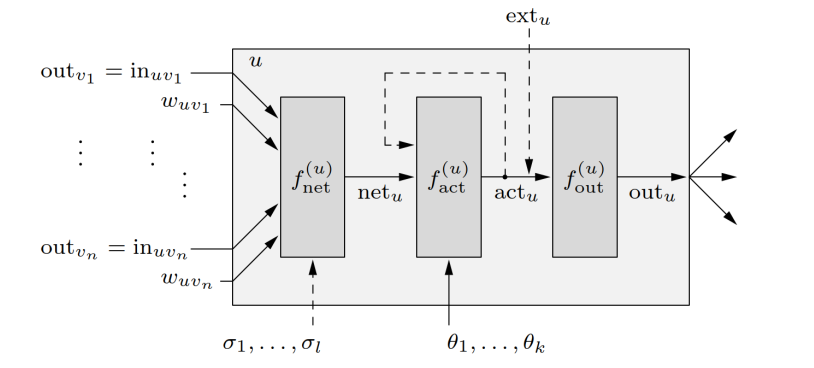
\includegraphics[scale=0.4]{img/ANN.png}
\caption{rappresentazione di un singolo neurone}
\label{fig:7}
\end{figure}

Ogni connessione $(u,v) \in C$ possiede un peso $w_{uv}$ che definisce l'importanza del dato originato da $v$ per il neurone $u$. Ad ogni neurone $u \in U$ vengono, invece, assegnate quattro variabili: il \emph{network input} $net_u$, la \emph{activation} $act_u$, l'\emph{output} $out_u$ e l'\emph{external input} $ext_u$ (vedi Figura \ref{fig:7}). Le prime tre variabili vengono calcolate in ogni momento dell'evoluzione dell'ANN grazie a tre funzioni associate:

\begin{enumerate}
\item{La \emph{network input function} $f^u_{net}$: calcola la somma pesata dell'input.}
\item{La \emph{activation function} $f^u_{act}$: ne esistono vari modelli (gaussiana, sigmoide, etc.) a seconda dell'applicazione.}
\item{La \emph{output function} $f^u_{out}$: definisce l'output a seconda che il neurone venga o meno attivato.}
\end{enumerate}

Se il grafo che rappresenta l'ANN è aciclico si parla di \emph{feed forward network} e la computazione procede in modo unidirezionale da $U_{(in)}$ a $U_{(out)}$ seguendo l'ordine topologico\footnote{L'ordine topologico è una numerazione dei vertici di un grafo diretto tale che tutti gli archi partano da un nodo associato ad un numero minore rispetto a quello associato al nodo di arrivo. Un ordine topologico esiste solo per grafi aciclici.} del network. Nel caso, invece, il grafo contenga un ciclo, allora si parla di \emph{recurrent network}.
I processi all'interno di un ANN si dividono in due fasi:

\begin{enumerate}
\item{La \emph{input phase}: dove gli input esterni vengono acquisiti dai neuroni di input.}
\item{La \emph{work phase}: dove i neuroni di input vengono spenti e un nuovo output viene computato da ogni neurone. La \emph{work phase} continua finchè gli output sono stabili o si raggiunge un timeout.}
\end{enumerate}

\begin{figure}
\centering
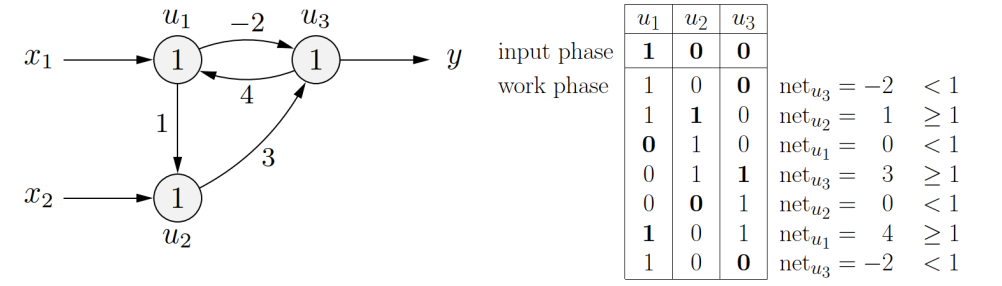
\includegraphics[scale=0.3]{img/rnn1.png}
\caption{computazione di una recurrent neural network che non giunge ad uno stato stabile}
\label{fig:8}
\end{figure}


Nel caso delle recurrent neural network, potrebbe accadere che non si giunga mai ad uno stato stabile a seconda di quale ordine di update dei neuroni si scelga di seguire. In Figura \ref{fig:8} abbiamo un esempio di una computazione con risultato oscillante in un recurrent neural network. L'ordine seguito per l'update è: $u_3,u_1,u_2,u_3,u_1,u_2\dots$. Se si fosse seguito un diverso ordine la computazione avrebbe raggiunto uno stato stabile.

\subsection{Training delle ANN}

Abbiamo visto in precedenza che è possibile allenare in modo automatico una singola TLU grazie alla delta rule. Come abbiamo già avuto modo di osservare questo procedimento non può essere generalizzato alle ANN. Tuttavia, i principi a cui ci ispiriamo sono i medesimi: calcolare correzioni ai pesi ed ai threshold dei singoli neuroni e aggiornarli di conseguenza. A seconda del tipo dei dati che utilizziamo per allenare le nostre ANN e dei criteri di ottimizzazione distiguiamo due tipi di apprendimento:

\begin{enumerate}
\item{\emph{fixed learning task} o apprendimento con supervisione}
\item{\emph{free learning task} o apprendimento senza supervisione}
\end{enumerate}

Nel caso di una fixed learning task avremo un insieme 
$L=\{(\ii_1,\oo_1),\dots,(\ii_n,\oo_n)\}$ di coppie che assegnano ad ogni input un output desiderato. Una volta completato il processo di apprendimento, la ANN dovrebbe essere in grado di restituire l'output adeguato rispetto all'input che le viene presentato. In pratica, questo accade raramente e bisogna accontentarsi di un risultato approssimativo.
Per giudicare in che misura una ANN si avvicina alla soluzione della fixed learning task si adotta una funzione di errore. Solitamente tale funziona viene calcolata come il quadrato della differenza tra l'output desiderato e quello attuale:
$$
e = \sum_{l \in L} \sum_{v \in U_{(out)}} e^l_v
$$
dove
$$
e^l_v = (o^l_v - out_v)^2
$$
è l'errore individuale per una particolare coppia $l$ e un neurone di output $v$. Il quadrato delle differenze viene scelto per vari motivi. Per prima cosa, errori positivi e negativi altrimenti si cancellerebbero a vicenda e non sarebbero presi in considerazione. In secondo luogo, questa funzione è ovunque derivabile, semplificando così il processo di aggiornamento dei pesi e dei threshold.
Nel free learning task avremo, invece, solo una sequenza di input $L = \{\ii_1, \dots, \ii_n\}$. Questo comporta che, a differenza del fixed learning task, non avremo modo di calcolare una funzione di errore rispetto ad un output atteso. In linea di principio, infatti, l'obiettivo di un free learning task sarà quello di produrre un output "simile" per input "simili". Un caso particolare potrebbe essere quello del \emph{clustering} dei vettori di input. 
Qualsiasi processo di apprendimento si scelga esistono alcune buone pratiche che è utile seguire. Una è quella di normalizzare il vettore di input. Comunemente lo si scala in modo tale che abbia media uguale a 0 e la varianza ad 1. Per fare questo uno deve calcolare per ogni neurone $u_k \in U_{(in)}$ la media aritmetica $\mu_k$ e la deviazione standard $\sigma_k$ degli input esterni:

$$
\mu_k = \frac{1}{|L|}\sum_{l \in L} ext^l_{u_k} \quad \quad \sigma_k = \sqrt{\frac{1}{|L|}\sum_{l \in L} (ext^l_{u_k} - \mu_k)^2}
$$

Quindi gli input esterni vengono ricalcolati secondo questa formula:

$$
ext^{new}_{u_k} = \frac{ext^{old}_{u_k} - \mu_k}{\sigma_k}
$$

\subsection{Multi-layer perceptrons}

\begin{figure}
\centering
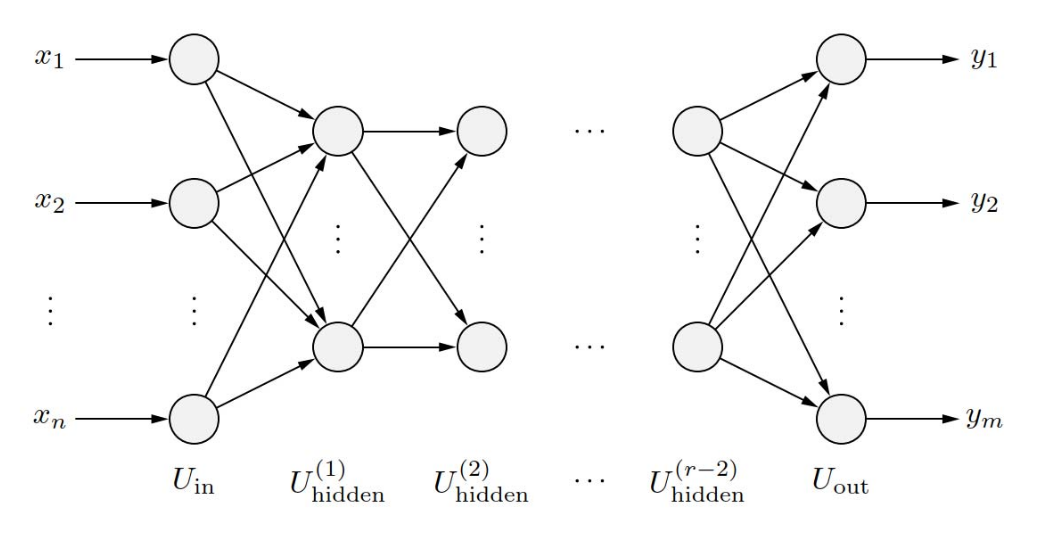
\includegraphics[scale=0.3]{img/MLP.png}
\caption{multi-layer perceptrons}
\label{fig:9}
\end{figure}


Una delle prime ANN sviluppate furono i \emph{multi-layer perceptrons} (nel seguito MLP). Le MLP sono particolari feed-forward network  in cui le unità base (i percettroni) sono organizzati in \emph{layer} e ogni layer ha connessioni solo con il layer successivo (vedi Figura \ref{fig:9}). Questo permette di minimizzare il fenomeno delle continue ricomputazioni che avverrebbero durante la propagazione del segnale nei normali feed-forward network.
La network input function di ogni neurone $u \in U_{(hidden)} \cup U_{(out)}$ viene calcolata come la somma pesata degli input, come:
$$
f^u_{net}(\ww_u,\ii_u) = \sum_{v \in pred(u)} w_{uv}out_v
$$
L'activation function, invece, è una così detta \emph{funzione sigmoide}, ossia una funzione monotona non decrescente tale che:
$$
f: \mathbb{R} \to [0,1] \quad \text{ con } \lim_{x\to-\infty}f(x) = 0 \quad \text{ e } \lim_{x\to\infty}f(x) = 1
$$

\begin{figure}

\begin{subfigure}{0.5\textwidth}
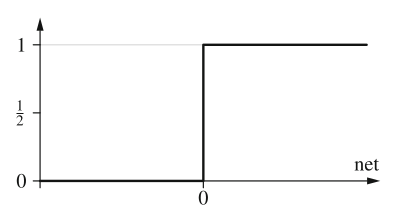
\includegraphics[width=0.9\linewidth, height=3cm]{img/step.png} 
\caption{step function}
\end{subfigure} %%
\begin{subfigure}{0.5\textwidth}
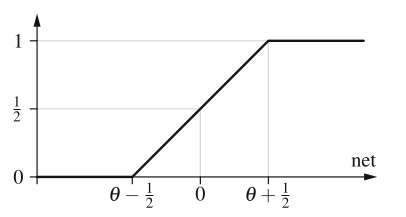
\includegraphics[width=0.9\linewidth, height=3cm]{img/semilinear.png}
\caption{semi-linear function}
\end{subfigure} 
\begin{subfigure}{0.5\textwidth}
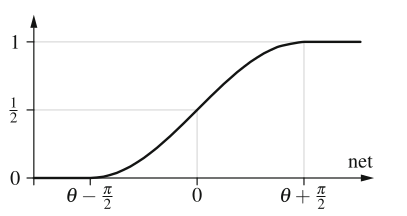
\includegraphics[width=0.9\linewidth, height=3cm]{img/sineup.png} 
\caption{sine up to saturation}
\end{subfigure}
\begin{subfigure}{0.5\textwidth}
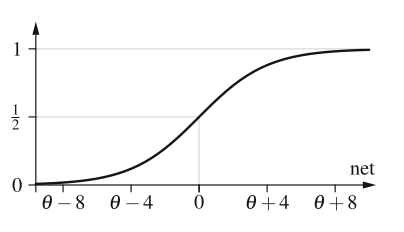
\includegraphics[width=0.9\linewidth, height=3cm]{img/logistic.png} 
\caption{logistic function}
\end{subfigure}


\caption{Alcune funzioni sigmoidi}
\label{fig:10}
\end{figure}

La funzione di output può essere sia una sigmoide oppure una semplice funzione lineare. \\
La struttura a layer di un MLP suggerisce che si possa descrivere il network con l'aiuto di una matrice dei pesi. In questo modo la computazione del MLP può essere rappresentata attraverso la moltiplicazione tra matrici e vettori. Tuttavia, noi non abbiamo utilizzato in classe una matrice per l'intero network, ma una per ogni singolo layer. Siano $U_1 = \{ v_1, \dots, v_n \}$ e $U_2 = \{ u_1, \dots, u_m \}$ due layer consecutivi di neuroni. I pesi delle loro connessioni sono codificati in una matrice $W$ di dimensioni $n \times m$:

$$
W = \begin{pmatrix}
  w_{u_1v_1} & w_{u_1v_2} & \cdots & w_{u_1v_n} \\
  w_{u_2v_1} & w_{u_2v_2} & \cdots & w_{u_2v_n} \\
  \vdots  & \vdots  & \ddots & \vdots  \\
  w_{u_mv_1} & w_{u_mv_2} & \cdots & w_{u_mv_n} 
 \end{pmatrix}
$$

Se due neuroni $u_i$ e $v_j$ non sono connessi, è sufficiente porre $w_{u_iv_j} = 0$. Il vantaggio di questa matrice sta nel fatto che è possibile scrivere il network input di un layer come:

$$
\mathbf{net}_{U_2} = W \mathbf{in}_{U_2} = W \mathbf{out}_{U_1}
$$

dove $\mathbf{net}_{U_2} = (net_{u_1}, \dots, net_{u_m})^\top$ e $\mathbf{in}_{U_2} = \mathbf{out}_{U_1} = (out_{v_1}, \dots, out_{v_n})^\top$. \\
Fino ad adesso abbiamo visto che le ANN possono rappresentare funzioni booleane, ma quando si parla di funzioni a valori continui? 


\begin{theorem}
Ogni funzione Riemann-integrabile è approssimata con precisione arbitraria da un MLP avente quattro layer.
\end{theorem}

\begin{figure}
\centering
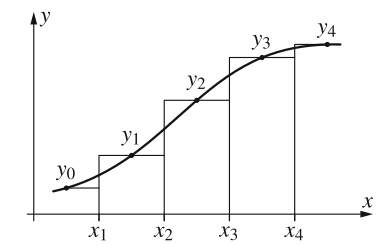
\includegraphics[scale=0.4]{img/approx.png}
\caption{Approssimazione di una funzione continua con una step function}
\label{fig:11}
\end{figure}

\begin{figure}
\centering
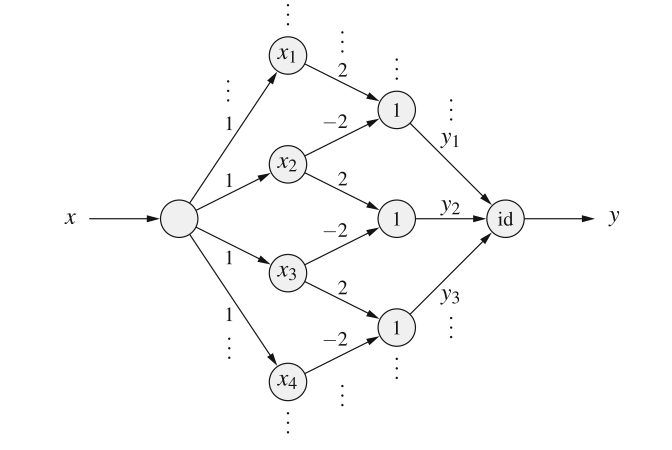
\includegraphics[scale=0.3]{img/riemann.png}
\caption{MLP che calcola la step function in Figura \ref{fig:11}}
\label{fig:12}
\end{figure}

Ogni funzione, infatti, può essere approssimata da una step function (come in Figura \ref{fig:11}). Ad ogni pivot $x_i$ associamo nel nostro MLP un neurone nel primo hidden layer (vedi Figura \ref{fig:12}). Nel secondo hidden layer creiamo un neurone per ogni scalino, il quale riceverà input dai due neuroni del primo livello che sono assegnati ai valori $x_i$ e $x_{i+1}$ che definiscono i bordi dello scalino. A questo punto, scegliamo pesi e threshold in modo tale che il neurone venga attivato se e solo se l'input è maggiore di $x_i$ e minore di $x_{i+1}$. Siccome la funzione di attivazione del neurone di output è la funzione di identità, il valore così calcolato viene emesso così come è ricevuto. 
Dovrebbe essere chiaro che l'approssimazione può crescere a piacere semplicemente aggiungendo neuroni e diminuendo la lunghezza dei gradini. Possiamo, inoltre, risparmiarci un layer se non utilizziamo nel calcolo l'altezza assoluta ma quella relativa come peso della connessione al neurone di output.
Bisogna notare, comunque, che questo risultato non ha natura costruttiva, ossia non ci dice come deve essere fatto un MLP che approssimi con una data accuratezza una certa funzione. Tutto ciò che afferma il Teorema 3 è che limitare il numero di layer non pregiudica la proprietà del MLP di essere un \emph{approssimatore universale}.

\subsection{Regressione}

Abbiamo visto che per allenare un ANN occorre minimizzare la funzione di errore, la quale si calcola solitamente come il quadrato della differenza tra output aspettato e attuale. Questo avvicina il problema dell'apprendimento nelle reti neurali a quello più generale della \emph{regressione}. La regressione è una tecnica molto usata in analisi e in statistica per estrapolare la retta (o, più in generale, il polinomio) che meglio approssima la relazione esistente in un insieme di dati/osservazioni. Detto in modo più formale, se $G = \{(\ww_0,y_0), \dots, (\ww_n,y_n)\}$ è il nostro dataset e immaginiamo esista una relazione funzionale tra il vettore di input $\ww_i$ e l'ascissa $y$, allora la regressione ci aiuterà a trovare i parametri di quella funzione. A seconda del diverso genere di funzione avremo diverse forme di regressione.

\subsubsection{Regressione lineare}

Se ci aspettiamo che le nostre due quantità $x$ e $y$ esibiscano una dipendenza lineare, allora dovremo identificare i parametri $a$ e $b$ che individuano la retta $y = g(x) = a + bx$. In generale, tuttavia, non sarà possibile trovare una singola retta che passi per tutti i punti del nostro dataset. Quello che faremo sarà trovare la retta che devi dai punti il meno possibile e che, quindi, minimizzi l'errore calcolato come segue: 

$$
F(a,b) = \sum(g(x_i) - y_i)^2 = \sum(a + bx_i - y_i)^2
$$

Il teorema di Fermat ci dice che una condizione necessaria perché un minimo della funzione $F(a,b)$ esista è che la derivata parziale in entrambi i parametri si annulli:

$$
\frac{\partial F}{\partial a} = \sum 2(a + bx_i - y_i) = 0
$$

$$
\frac{\partial F}{\partial b} = \sum 2(a + bx_i - y_i)x_i = 0
$$

Questo sistema può essere risolto con alcune semplici tecniche di algebra lineare (vedi pag. 174 del libro). La soluzione così trovata sarà unica a meno che ogni valore $x_i$ sia identico. 

\subsubsection{Regressione polinomiale e multilineare}

Il metodo precedente può essere esteso in modo ovvio a polinomi di ordine arbitrario. In questo caso, si prende come ipotesi che la funzione indotta dal dataset approssimi un polinomio di ordine $n$:

$$
y = p(x) = a_o + a_1x + \dots + a_nx^n
$$

E si cercherà di minimizzare la funzione $F$ tale che:

$$
F(a_1,\dots,a_n) = \sum(p(x_i) - y_i)^2 = \sum(a_o + a_1x + \dots + a_nx^n -y_i)^2
$$

Come nel caso della regressione lineare, la funzione potrà essere minimizzata solo se le derivate parziali rispetto ai parametri $a_i$ si annullano:

$$
\frac{\partial F}{\partial a_1} = 0 \quad \dots \quad \frac{\partial F}{\partial a_n} = 0
$$

Inoltre, non siamo limitati a calcolare funzioni ad un solo argomento. Con alcune minori modifiche questo metodo è capace di approssimare funzioni in un numero arbitrario di argomenti. In quel caso, la chiameremo \emph{regressione multilineare}.

\subsubsection{Regressione logistica}

Nel situazione in cui il nostro dataset non sia approssimato con sufficiente accuratezza da una funzione polinomiale, potremmo dover utilizzare funzioni di generi diversi. Data, per esempio, una funzione della forma:

$$
y = ax^b
$$

possiamo trasformarla in una equazione lineare applicando l'operazione di logaritmo:

$$
ln(y) = ln(a) + b \cdot ln(x)
$$

Nel caso delle ANN ci interessiamo in particolare alla funzione logistica (vedi Figura \ref{fig:10}(d)):

$$
y = \frac{Y}{1 + e^{a+bx}}
$$

Siccome molte ANN utilizzano come funzione di attivazione del neurone proprio la funzione logistica, se trovassimo un modo di applicarci il metodo della regressione potremmo determinare i parametri di qualsiasi network a due layer con un unico input. Il valore $a$ nella funzione corrisponderebbe al threshold del neurone di output e la $b$ al peso dell'input. Possiamo "linearizzare" la funzione logistica applicandoci le seguenti trasformazioni (comunemente chiamata \emph{logit transformation}):

$$
y = \frac{Y}{1 + e^{a+bx}} \leftrightarrow \frac{1}{y} = \frac{1 + e^{a+bx}}{Y} \leftrightarrow \frac{Y - y}{y} = e^{a+bx} \leftrightarrow ln(\frac{Y - y}{y}) = a+bx
$$

Se estendiamo il nostro approccio fino a comprendere funzioni con più argomenti, in analogia a quanto accade nella regressione multilineare, possiamo utilizzarlo per computare i pesi di network a due layer con arbitrari neuroni di input. Tuttavia, siccome il metodo della somma degli errori funziona solo quando parliamo di neuroni di output, questo approccio non può essere esteso a network con più di due layer.

\subsection{Backpropagation}

Come abbiamo appena visto la regressione logistica funziona solo per MLP con due layer di neuroni. Un approccio più generale è quello del \emph{gradient descent}. Il metodo consiste nell'utilizzare la funzione di errore per calcolare la direzione in cui cambiare i pesi e il threshold per minimizzare l'errore. Condizione necessaria per il suo utilizzo è che la funzione sia differenziabile. Tuttavia, un MLP ha una funzione logistica come funzione di attivazione e, quindi, la funzione di errore sarà differenziabile (posto che la funzione di output sia la funzione identità).
Intuitivamente, il \emph{gradiente} descrive la pendenza di una funzione. Questo è calcolato assegnando ad ogni punto del dominio della funzione un vettore, i cui componenti sono le derivate parziali rispetto ai agli argomenti(un esempio in Figura \ref{fig:13}). L'operazione di calcolare il gradiente (di un punto o di una funzione) è comunemente denotata con l'operatore differenziale $\nabla$ (pronuncia: nabla).

\begin{figure}
\centering
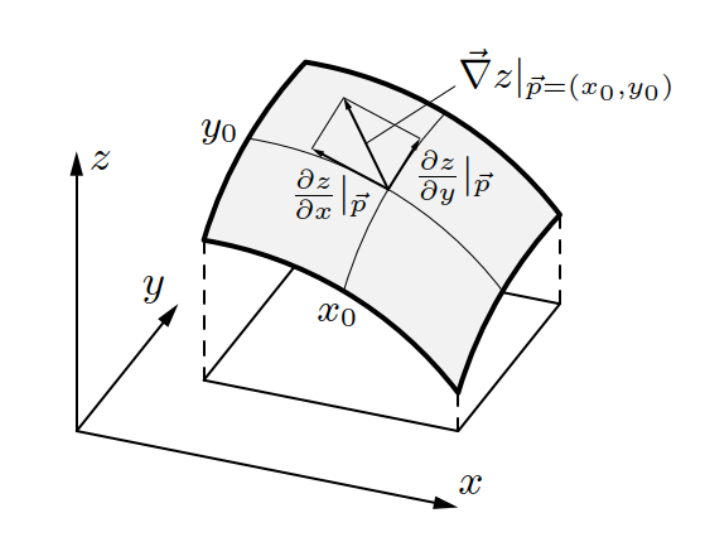
\includegraphics[scale=0.3]{img/gradient.png}
\caption{Il gradiente di una funzione a due argomenti.}
\label{fig:13}
\end{figure}

Nel caso delle MLP, calcolare il gradiente della funzione di errore si traduce nel calcolare la derivata parziale della funzione di errore rispetto ai pesi e i threshold presi come parametri. Sia $\ww_u = (-\theta,w_{u_1},\dots,w_{u_k})$ il vettore dei pesi di un singolo layer esteso così da includere anche il threshold, calcoliamo il gradiente come segue:
$$
\nabla_{\ww_u} e = \frac{\partial e}{\partial \ww_u} = (-\frac{\partial e}{\partial \theta}, \frac{\partial e}{\partial w_{u_1}},\dots,\frac{\partial e}{\partial w_{u_k}})
$$
Siccome l'errore totale $e$ è dato dalla somma degli errori individuali rispetto a tutti i neuroni e tutti i training pattern $l$, otteniamo che:
$$
\nabla_{\ww_u} e = \frac{\partial e}{\partial \ww_u} = \frac{\partial}{\partial \ww_u} \sum_{l \in L} e^l = \sum_{l \in L} \frac{\partial e^l}{\partial \ww_u}
$$
\begin{remark}
\emph{Se abbiamo come $f_{(act)}$ la funzione logistica avremo che i cambiamenti operati sul vettore $\ww_u$ saranno proporzionali alla derivata della funzione $f_{(act)}$. Più vicini allo 0 della funzione sono i valori, più ripido sarà il pendio della funzione e, per tanto, più rapido sarà l'apprendimento.}
\end{remark}

Come facciamo dopo aver trovato l'errore a calcolare la correzione necessaria per ogni peso e threshold di ogni singolo neurone? Il processo che ci permette di fare questo viene chiamato \emph{error backpropagation} ed è schematizzato in Figura \ref{fig:14}. Si assume che la funzione di attivazione sia la funzione logistica per ogni neurone $u \in U_{(hidden)} \cup U_{(out)}$ tranne che per quelli di input.

\begin{figure}
\centering
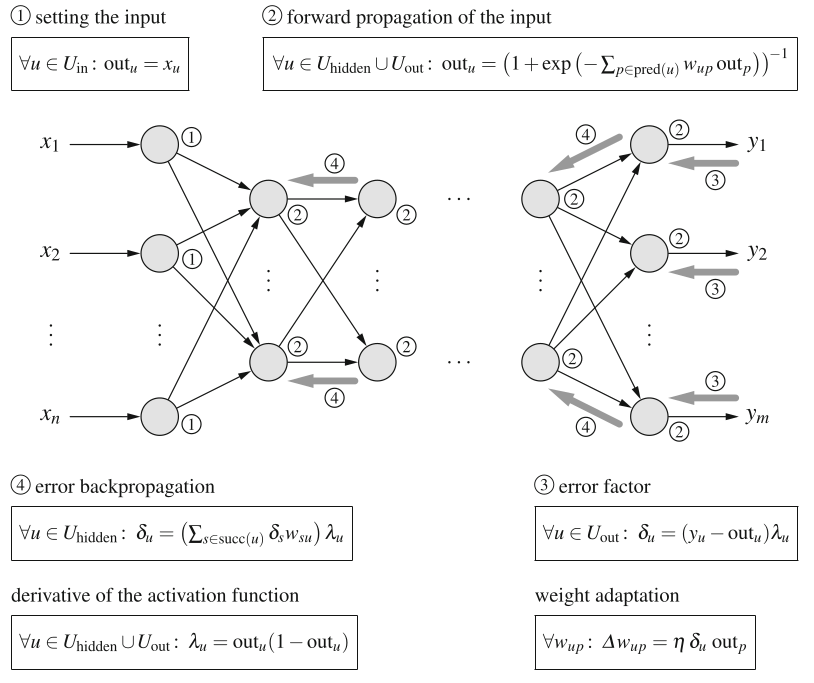
\includegraphics[scale=0.4]{img/backpropagation.png}
\caption{Propagazione dell'errore in un MLP.}
\label{fig:14}
\end{figure}

Inizialmente, (1) applichiamo l'input ai neuroni di input che lo restituiscono senza modifiche in output al primo dei layer hidden. (2) Calcoliamo per ogni neurone dei seguenti layer la somma pesata degli input e al risultato applichiamo la funzione logistica generando così l'output che verrà propagato in tutto il network fino ai neuroni terminali. A questo punto, (3) calcoliamo la differenza tra l'output atteso e quello attuale e, dato che la funzione di attivazione è invertibile, risaliamo dal vettore di errore a quale fosse l'input che ha condizionato quel particolare errore (la variabile $\delta_u$, nell'immagine). Avendo, ora, (4) trasformato l'errore della variabile di output $out_u$ in quello della variabile di input $net_u$ possiamo distribuire l'errore (e la correzione necessaria) in modo proporzionale al ruolo del singolo neurone nel calcolo del seguente output. Propago a ritroso l'errore fino ai neuroni di input. Bisogna osservare comunque che data la forma della funzione logistica l'errore non può sparire completamente, in quanto il gradiente approssimerà il vettore nullo più si avvicinerà allo zero. 

\begin{remark}
\emph{Se si inizializza il learning rate $\eta$ ad un valore troppo alto, al posto di discendere la curva si corre il rischio di saltare da un "picco" della funzione all'altro senza convergere mai al minimo. Inoltre, non è affatto detto che il minimo raggiunto in questo modo sia il minimo globale della funzione. La causa sarà piuttosto da ascrivere alla scelta dei valori iniziali. Una soluzione al problema può essere quella di ripetere l'apprendimento, inizializzando il sistema con una diversa configurazione di pesi e threshold, e scegliere alla fine quale configurazione risulta in un miglior minimo.}
\end{remark}

\subsubsection{Variazioni sul gradient descent}

Esistono varie sofisticazioni della tecnica del gradient descent che permettono un più veloce apprendimento e, nello stesso momento, un miglior controllo sulla lunghezza dei singoli step di apprendimento. Alcuni esempi sono:

\begin{itemize}
\item{\emph{Manhattan training}: utilizza al posto del valore del gradiente solo il suo segno per calcolare la direzione. Questo permette di semplificare notevolmente la computazione.}
\item{\emph{Flat spot elimination}: cerca di limitare l'abbattimento della lunghezza degli step di apprendimento quando ci si avvicina ad un plateau della funzione "sollevando" artificialmente la derivata della funzione in quel punto.}
\item{\emph{Momentum term}: ad ogni successivo step aggiungo al gradiente una frazione del precedente cambiamento di pesi così da avere una memoria di quanto velocemente stava cambiando nel passato.}
\item{\emph{Self-adaptive error backpropagation}: permetto ad ogni parametro di avere un diverso learning rate in modo da avere un più fine controllo rispetto alle caratteristiche del singolo parametro.}
\item{\emph{Resilient error backpropagation}: combina il Manhattan training con l'approccio self-adaptive.}
\item{\emph{Quick propagation}: al posto di utilizzare il gradiente approssimo la funzione con una parabola e salto direttamente all'apice della parabola.}
\item{\emph{Weight decay}: riduce i pesi per evitare di rimanere intrappolato in una regione già saturata.}
\end{itemize}

\subsubsection{Overfitting e underfitting}

Quanti neuroni ho bisogno per avere un buon network? Come regola di massima si dovrebbe scegliere il numero di neuroni negli hidden layer seconda la seguente formula:
$$
\# \text{hidden neurons} = (\# \text{input neurons} + \# \text{output neurons})/2
$$
Non esiste una spiegazione teoretica soddisfacente del perché questo sia un buon numero, ma è stato dimostrato empiricamente. Se, infatti, il numero dei neuroni negli hidden layer è troppo basso rischiamo l'\emph{underfitting}, ossia che il nostro MLP non riesca ad approssimare in modo soddisfacibile la complessità della funzione che vogliamo catturare. Al contrario se ne ho troppi rischio di incorrere nell'\emph{overfitting}, ossia che il nostro MLP si adatti agli esempi che gli abbiamo fornito durante il periodo di apprendimento, ma anche alle loro specificità accidentali (errori e deviazioni).
Per evitare questi fenomeni è buona pratica dividere il nostro data set in modo da avere due sottoinsiemi di dati: alcuni dati per l'apprendimento ed altri per la validazione del processo di apprendimento. I primi verranno usati per allenare il nostro network e i secondi per giudicare se effettivamente il network approssimi la funzione desiderata. \'E possibile iterare a piacere questo procedimento suddividendo i dati non in due sottoinsiemi, ma in un numero arbitrario, così da ottenere una conferma incrociata dei progressi nell'apprendimento del nostro network.
Un diverso metodo per evitare l'overfitting è quello di terminare l'apprendimento quando il differenziale dell'errore tra un epoca ed un altra si abbassi sotto una certa soglia, oppure se l'apprendimento si protrae per un periodo troppo lungo.

\subsubsection{Sensitivity analysis}

Uno svantaggio delle ANN è che la conoscenza risultante dal processo di apprendimento è codificata in matrici a valori reali e, quindi, di difficile comprensione per l'utente. Abbiamo mostrato una interpretazione geometrica dei processi interni alle ANN, ma tale interpretazione, sebbene sia generalizzabile ad ANN arbitrariamente complesse, offre poco aiuto all'intuizione quando lo spazio degli input supera le tre dimensioni. Una soluzione a questo problema è quella di operare una \emph{sensitivity analysis}, la quale determinerà l'influenza dei vari input sull'output del network. Per eseguirla occorrerà calcolare la somma delle derivate parziali degli output rispetto agli input esterni per ogni neurone di output e ogni training pattern. Questa somma viene, infine, divisa per il numero di training pattern, per rendere la misura indipendente dalla grandezza del dataset.

$$
\forall u \in U_{(in)}: \quad s(u) = \frac{1}{|L|} \sum_{l \in L} \sum_{\nu \in U_{(out)}} \frac{\partial out_\nu^l}{\partial ext_u^l}
$$

Il valore $s(u)$ risultante indica quanto importante fosse l'input assegnato al neurone $u$ per la computazione del MLP. Grazie a questa considerazione potremmo decidere di semplificare il network eliminando i nodi con i valori di $s(u)$ più bassi.

\subsection{Deep learning}

Il Teorema 3 ha mostrato come un MLP con un solo hidden layer può approssimare ogni funzione continua su $\mathbb{R}^n$ con una precisione arbitraria. Questo risultato, tuttavia, non ha natura costruttiva e può non essere semplice conoscere a priori il numero esatto di neuroni necessari per approssimare una data funzione. Inoltre, a seconda della funzione, questo numero potrebbe assumere dimensioni considerevoli!
Un esempio è quello della funzione che calcola la parità su una parola di $n$-bit. L'output sarà 1 se e solo se nel vettore di input che rappresenta la parola saranno ad 1 un numero pari di bit. Nel caso scegliessimo di utilizzare un MLP con un solo hidden layer questo avrà al suo interno $2^{n-1}$ neuroni, in quanto la forma normale disgiuntiva della funzione di parità su $n$-bit è una disgiunzione di $2^{n-1}$ congiunzioni. 
Se permettiamo, invece, di avere più di un layer, il numero di neuroni crescerà in modo lineare alla dimensione dell'input. Questa constatazione ha portato allo sviluppo del così detto \emph{deep learning}, dove la "profondità" è quella del più lungo cammino che separa i neuroni di input da quelli di output. Il razionale è quello di permettere una maggiore profondità del network in cambio di un miglioramento delle risorse utilizzate nel calcolo e nella costruzione. Il deep learning oltre ad offrire vantaggi porta con se alcune problematiche:

\begin{itemize}
\item{\emph{Overfitting}: l'incremento nel numero di neuroni dovuto alla presenza dei molti layer può avere l'effetto di moltiplicare i parametri in modo sproporzionato.}
\item{\emph{Vanishing gradient}: durante la propagazione dell'errore il grandiente si riduce dopo ogni layer fino a scomparire.}
\end{itemize}

Alcune soluzioni al problema dell'overfitting sono:

\begin{itemize}
\item{\emph{Weigth decay}, ossia mettere un tetto massimo ai valori che possono assumere i pesi per prevenire un adattamento troppo pedissequo al dataset.}
\item{\emph{Sparsity constraint}: si introducono dei limiti al numero di neuroni negli hidden layer, oppure si limita il numero di quelli attivi.}
\item{\emph{Dropout training}: alcuni neuroni degli hidden layer vengono omessi durante l'evoluzione del network.}
\end{itemize}

\begin{figure}
\centering
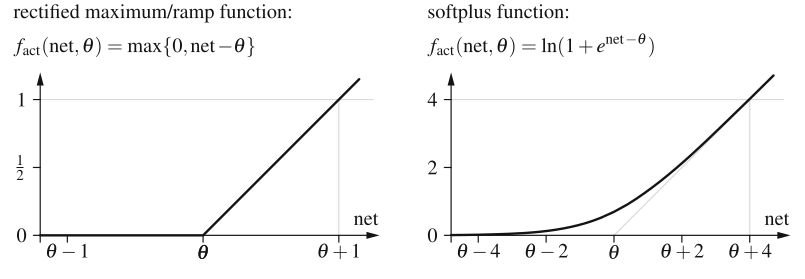
\includegraphics[scale=0.4]{img/relu.png}
\caption{Funzioni di attivazione sempre crescenti.}
\label{fig:15}
\end{figure}

Il problema del vanishing gradient è dato dal fatto che la funzione di attivazione è una funzione logistica la cui derivata raggiunge al massimo il valore di $\frac{1}{4}$. Di conseguenza, ogni propagazione dell'errore ad un layer precedente vi aggiunge un valore, spesso molto minore di 1, riducendo così il gradiente. Una soluzione è quella di modificare leggermente la funzione di attivazione in modo che sia sempre crescente. Alcuni candidati proposti in letteratura sono la \emph{ramp function} e la \emph{softplus function} (vedi Figura \ref{fig:15}).
Un approccio completamente diverso è quello di costruire il network "layer a layer". Una tecnica molto usata è quella di pensare al network come una pila di \emph{autoencoder}. Un autoencoder è un MLP che mappa il suo input in una sua approssimazione, utilizzando un hidden layer di dimensioni minori. Il layer nascosto funge da encoder per la codifica dell'input in una sua rappresentazione interna che è a sua volta decodificata dal layer di output. L'autoencoder, avendo un solo layer, non soffre delle stesse limitazioni e può essere allenato attraverso la normale backpropagation. Un problema con questo approccio è che se ci sono tanti neuroni negli hidden layer quanti quelli di input si rischia di propagare con minori aggiustamenti il segnale senza che l'autoencoder estragga alcuna informazione utile dal dato.
Esistono tre principali soluzioni:
\begin{itemize}
\item{\emph{Sparse autoencoder}: prevede di utilizzare un numero molto minore di neuroni nel hidden layer, rispetto a quelli di input. L'autoencoder sarà così costretto ad estrarre dall'input qualche feature interessante al posto di propagare semplicemente il dato.}
\item{\emph{Sparse activation scheme}: in modo simile a quanto si faceva per evitare l'overfitting, si decide di "spegnere" alcuni neuroni durante la computazione.}
\item{\emph{Denoising autoencoder}: si aggiunge randomicamente rumore all'input.}
\end{itemize}
Per ottenere un MLP con molteplici layer si combinano diversi autoencoder. Inizialmente si allena un singolo autoencoder. A quel punto, si rimuove il decoder e viene conservato solo il layer interno. Si utilizzano i dati preprocessati da questo primo autoencoder per allenarne un secondo, e così via fino a che si raggiunga un numero soddisfacente di layer.
MLP costruiti in questo modo sono risultati molto efficaci nel riconoscere con successo numeri scritti a mano. Se si volessero utilizzare dei network simili per una più ampia classe di applicazioni, dove, per esempio, le feature riconosciute dai layer interni non sono localizzate in una porzione specifica dell'immagine, bisognerebbe rivolgersi ai \emph{convolutional neural network} (più avanti, CNN). Questa architettura è ispirata al funzionamento della retina umana, in cui i neuroni adibiti alla percezione hanno un campo ricettivo, ossia una limitata regione in cui rispondono agli stimoli. Questo viene simulato nelle CNN connettendo i neuroni del primo hidden layer solo ad alcuni neuroni di input. I pesi vengono condivisi così che i vari network parziali possano essere valutati da differenti prospettive dell'immagine. Durante la computazione si procederà poi a muovere il "campo ricettivo" sulla totalità dell'immagine. Come risultato si ottiene una convoluzione della matrice dei pesi con l'immagine in input.

\subsection{Radial basis function network}

I così detti \emph{radial basis function network} (in quello che segue, RBFN) sono feed-forward network aventi tre layer di neuroni. Sono strutture alternative rispetto ai classici MLP. La differenza principale sta nella diversa scelta riguardo la funzione di attivazione. Se nel caso degli MLP avevamo una funzione sigmoide, ora avremo una funzione radiale di base \footnote{Una funzione radiale di base, o funzione di base radiale è una funzione a valori reali $f(x)$ il cui valore dipende unicamente tra la distanza dell'argomento $x$ e un punto prefissato $c$. Se il punto $c$ in questione è l'origine si dicono funzioni radiali.}. La $f_{net}$ dei neuroni di output è la somma pesata dei loro input, come in precedenza. Invece, per i neuroni nel hidden layer avremo che $f_{net}$ sarà uguale alla distanza tra il vettore di input e il vettore dei pesi. La funzione distanza che sceglieremo sarà una metrica in senso geometrico, e, per tanto, deve rispettare i seguenti tre assiomi:
$$
d(\ww,\vv) = 0 \leftrightarrow \ww = \vv
$$
$$
d(\ww,\vv) = d(\vv,\ww)
$$
$$
d(\ww,\ee) + d(\ee,\vv) \geq d(\ww,\vv)
$$
Una famiglia di funzioni usate spesso nelle applicazioni è quella formulata dal matematico prussiano Hermann Minkowski e battezzata in suo onore famiglia di Minkowski. Tale famiglia è definita come:
$$
d(\ww,\vv)_k = (\sum (w_i - v_i)^k)^{\frac{1}{k}}
$$
Alcuni esempi famosi di funzioni appartenenti alla famiglia sono:
$$
k = 1: \text{Manhattan distance}
$$
$$
k=2:\text{Euclidian distance}
$$
$$
k = \infty: \text{Maximum distance, ovvero } d(\ww,\vv)_\infty = max |w_i - v_i|
$$
\begin{figure}
\centering
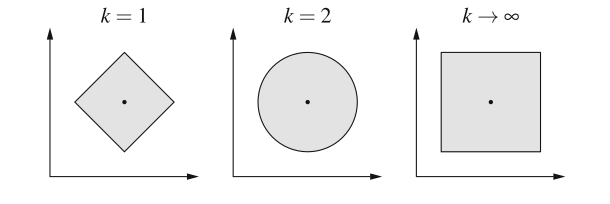
\includegraphics[scale=0.4]{img/circle.png}
\caption{Cerchi rispetto alle diverse definizioni di distanza.}
\label{fig:16}
\end{figure}
Un modo utile di visualizzare queste funzioni è quello di vedere che forma assume un cerchio a seconda delle varie metriche (vedi Figura \ref{fig:16}). La ragione è che un cerchio è definito come quell'insieme di punti che stanno alla stessa distanza da un dato punto. Variando la definizione di distanza, varia la forma che assume il cerchio nei diversi spazi.
Passando ora a considerare $f_{act}$ avremo, nel caso dei neuroni di output, una funzione lineare. Invece, per i neuroni del hidden layer avremo una funzione monotona decrescente tale che:
$$
f: \mathbb{R}^{+} \to [0,1] \quad \text{con} \quad f(0) = 1 \quad \text{e} \quad \lim_{x \to \infty} f(x) = 0
$$
Questa funzione calcola l'area in cui il neurone focalizza la propria attenzione definita dal raggio di riferimento $\sigma$. I vari parametri e la forma della funzione determinano l'ampiezza di questa area. Le funzioni più utilizzate per determinare l'area di attivazione sono quelle riportate in Figura \ref{fig:17}.
\begin{figure}
\centering
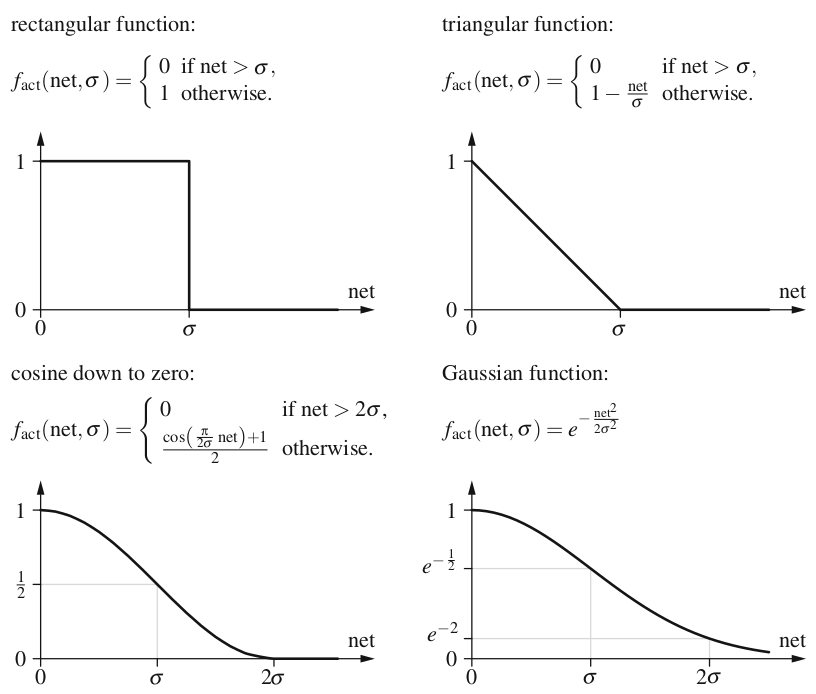
\includegraphics[scale=0.3]{img/act_rbf.png}
\caption{Varie funzioni di attivazione per un RBFN.}
\label{fig:17}
\end{figure}
Come esempio, applichiamo un RBFN per simulare una congiunzione booleana. Un network che risolve il problema è quello costituito da un singolo neurone hidden, il cui vettore dei pesi (il centro della funzione radiale) è esattamente il punto in cui in output vorremo il valore \emph{vero}, ovvero (1,1). Il raggio $\sigma$ sarà posto a $\frac{1}{2}$ e verrà codificato nel threshold del neurone. La funzione di distanza usata è quella euclidea e come $f_{act}$ utilizziamo una funzione rettangolare. Il diagramma in Figura \ref{fig:18} offre una rappresentazione grafica di quanto detto. 
\begin{figure}
\centering
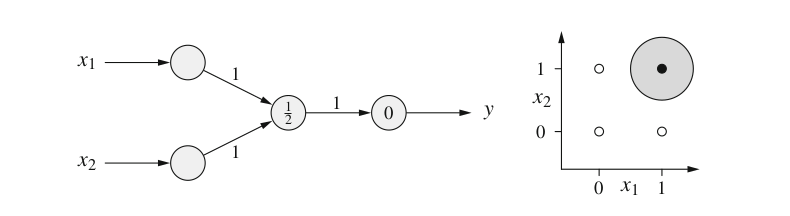
\includegraphics[scale=0.4]{img/and_rbf.png}
\caption{RBFN che calcola la congiunzione booleana.}
\label{fig:18}
\end{figure}
In generale, un RBFN ha lo stesso potere espressivo di un MLP e può essere visto come un approssimatore universale, ovvero può approssimare (con errore arbitrariamente piccolo) una qualsiasi funzioni Riemann-integrabile. Il procedimento è lo stesso che nel caso degli altri network: la funzione viene approssimata da una funzione a scalini che può essere calcolata facilmente da una funzione radiale se la definiamo come la somma pesata di funzioni rettangolari. L'approssimazione può essere migliorata aumentando il numero dei punti in cui si valuta la funzione. Inoltre, se al posto della funzione rettangolare, viene utilizzata una funzione Gaussiana possiamo ottenere delle transizioni più "morbide" evitando bruschi salti. 

\subsection{Training delle RBFN}

Se negli altri ANN la fase di inizializzazione era triviale, in quanto bastava scegliere valori in modo casuale, quando si tratta di RBFN lo stesso approccio conduce a risultati subottimali. Consideriamo, quindi, il caso speciale delle \emph{simple radial basis function network}, dove ogni esempio di apprendimento viene associato ad una propria funzione radiale. Dato un fixed learning task $L = \{l_1,\dots,l_m\}$, avente $m$ pattern $l = (\ii^l,\oo^l)$, definiremo il vettore dei pesi associato al neurone $v_k$ come:

$$
\forall k \in \{1,\dots,m\}: \ww_{v_k} = \ii_k
$$

Assumendo una funzione di attivazione gaussiana, il raggio $\sigma_k$ è inizializzato in accordo a questa euristica:

$$
\forall k \in \{1,\dots,m\}: \sigma_k = \frac{d_{max}}{\sqrt{2m}}
$$

Dove $d_{max}$ è la massima distanza tra i vettori di input. Questa scelta permette di centrare le varie gaussiane in modo che non si sovrappongano l'una all'altra, ma si distribuiscano in modo ordinato rispetto allo spazio di input. Per quanto riguarda, invece, i pesi dei neuroni di output, vengono calcolati secondo la seguente funzione:
$$
\forall u: \sum_{k=1}^m w_{u_k} out_{u_k} - \theta  = o_u
$$
Ponendo $\theta = 0$, avremo che la precedente equazione è equivalente a:
$$ 
\mathbf{A}\cdot \ww_u = \oo_u
$$
Dove $\mathbf{A}$ è la matrice $m \times m$ che ha come componenti i vari output dei neuroni nel hidden layer. Se la matrice $\mathbf{A}$ ha rango completo, possiamo invertirla e calcolare il vettore dei pesi come segue:
$$
\ww_u = \mathbf{A}^{-1}\cdot \oo_u
$$
Questo metodo garantisce una perfetta approssimazione. Non è necessario, quindi, allenare un simple radial basis function network. In generale, se non vogliamo avere per ogni training pattern un neurone, dovremo selezionare $k$ sottoinsiemi del dataset e trovare, per ogni sottoinsieme, un rappresentante che  assoceremo ad un neurone nel layer hidden. In analogia a quanto accade nel caso "semplice" avremo una matrice $\mathbf{A}$ di dimensione $m\times (k+1)$ con i valori in output dei vari neuroni nel hidden layer. Dato che la matrice non è quadrata, non è possibile calcolarne l'inversa come avevamo fatto in precedenza. Tuttavia, esiste una alternativa chiamata la \emph{matrice pseudo-inversa}\footnote{La matrice pseudo-inversa $\mathbf{A}^+$ della matrice $\mathbf{A}$ è calcolata come $\mathbf{A}^+ = (\mathbf{A}^{\top}\mathbf{A})^{-1}\mathbf{A}^{\top}$.} che permette di completare il calcolo con una buona approssimazione. Ovviamente, l'accuratezza del network costruito in questo modo dipenderà dalla precisione con cui si scelgano i rappresentati delle varie sottoclassi del dataset. Esistono vari metodi per fare questo:
\begin{itemize}
\item{Scegliamo tutti i punti del dataset come centri. In questo caso ricadiamo nel caso "semplice" e i valori di output possono essere calcolati precisamente. Tuttavia, il calcolo dei pesi può risultare infattibile.}
\item{Costruiamo un sottoinsieme randomico per rappresentare i centri. Questo metodo ha il pregio di essere facilmente calcolabile. La performance, però, dipenderà dalla fortuna di scegliere dei "buoni" centri.}
\item{Utilizziamo un algoritmo di clustering (c-means clustering,learning vector quantization..)}
\end{itemize}


\begin{remark}
\emph{L'algoritmo c-means sceglie randomicamente $c$ centri di altrettanti cluster. Quindi il dataset viene partizionato in $c$ sottoclassi a seconda della vicinanza ai vari centri. In un passo successivo si calcola il "centro di gravità" del cluster così trovato e lo si elegge come nuovo centro. Si ricomputa l'appartenza dei punti del dataset e si procede così fino a che i centri smettono di oscillare.}
\end{remark}

La fase di training avviene come nel caso dei MLP attraverso gradient descent e backpropagation. 

\subsection{Learning vector quantization}

Fino ad ora ci siamo concentrati sui fixed learning task per descrivere l'apprendimento delle ANN: il successo dell'apprendimento si misura dall'adeguatezza con cui il network approssima gli output desiderati. Tuttavia, non sappiamo sempre quale output aspettarci per ogni input nel nostro dataset. L'obiettivo di una rete neurale in questi casi sarà quello di classificare o clusterizzare\footnote{Solitamente si usa il termine "classe" quando queste sono conosciute \emph{a priori}, dove, invece, i "cluster" sono derivati \emph{a posteriori} dai dati in base alle loro similitudini.} i dati in input, senza avere un'indicazione su cosa si stia cercando. La \emph{learning vector quantization} è una tecnica che ci aiuta ad operare il raggruppamento in modo automatico, trovando una adeguata tassellazione dello spazio di input. Come nel caso dell'algoritmo c-means, i vari cluster verranno rappresentati da punti detti "centri" scelti tra quelli del dataset.

\subsubsection{Learning vector quantization network}

Per calcolare la learning vector quantization utilizzeremo un network feed-forward a due layer che chiameremo \emph{learning vector quantization network} (in quel che segue, LVQN). Questo tipo particolare di network può essere visto come un RBFN che ha il layer di output al posto del hidden layer. Come nel caso dei RBFN avremo, infatti, che la funzione di input del layer di output è una funzione della distanza del vettore di input e quello dei pesi. Allo stesso modo, la funzione di attivazione dei neuroni di output è una funzione radiale. La differenza, nel caso dei LVQN, risiede nella $f_{(out)}$ dei neuroni di output, la quale non è la semplice identità, ma propaga il messaggio solo se l'attivazione del neurone è la massima tra le attivazioni dei neuroni di output. Se più di un'unità ha il valore massimo ne viene scelta una a random, mentre le altre vengono poste a zero (principio del \emph{winner-takes-all}). 

$$
f^u_{out} (act_u) = \begin{cases}
					1 \quad \text{if } act_u = \max_{v \in U_{out}} act_v\\
					0 \quad \text{altrimenti}
					\end{cases}
$$

Un'altra differenza rispetto all'algoritmo c-means riguarda il metodo attraverso cui i "centri" vengono aggiornati. In questo caso, infatti, i punti nel dataset vengono processati uno ad uno. La procedura viene chiamata \emph{competitive learning}: ogni input viene "conteso" dai vari neuroni di output, e viene vinto dal neurone con il valore di attivazione più alto. Il neurone vincitore viene adattato, in modo che il vettore di riferimento venga mosso più vicino al punto, dove, invece, il resto dei vettori di riferimento vengono allontanati dal punto (vedi Figura \ref{fig:19}). Questo viene fatto secondo le seguenti regole:

\begin{itemize}
\item{\emph{Attraction rule}: $
\mathbf{r}^{new} = \mathbf{r}^{old} + \eta(\mathbf{x} - \mathbf{r}^{old})
$} 
\item{\emph{Repulsion rule}: $
\mathbf{r}^{new} = \mathbf{r}^{old} - \eta(\mathbf{x} - \mathbf{r}^{old})
$} 
\end{itemize}

\begin{figure}
\centering
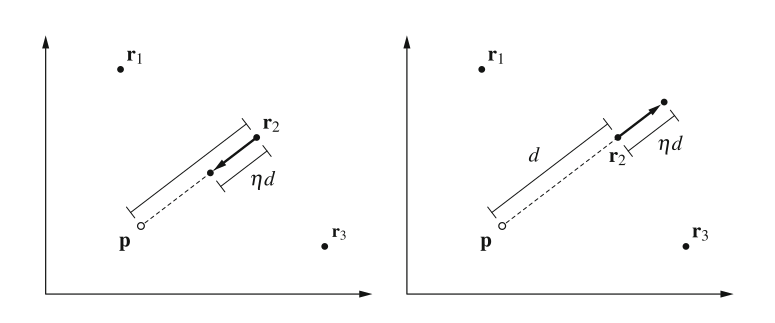
\includegraphics[scale=0.4]{img/adapt.png}
\caption{Attraction rule e repulsion rule in azione.}
\label{fig:19}
\end{figure}

dove $\mathbf{x}$ è l'input, $\mathbf{r}$ è il vettore di riferimento per il neurone vincitore e $\eta$ è il learning rate. Fino ad ora abbiamo sottointeso che il learning rate rimanesse fisso per la durata dell'apprendimento, tuttavia esistono delle situazioni in cui un learning rate costante può portare ad alcuni problemi. Un caso è quello rappresentato nel riquadro a sinistra della Figura \ref{fig:20}, dove il vettore di riferimento oscilla ciclicamente verso uno dei quattro punti. Un metodo semplice per risolvere il problema è quello di far decrescere il learning rate al crescere delle iterazioni (\emph{time dependent leanring rate}). In questo modo, il movimento circolare collassa col passare del tempo in una spirale, facendo così convergere l'algoritmo.
Un altro problema con la versione classica di questo algoritmo è che il processo di adattamento porti i vettori di riferimento ad allontanarsi sempre di più tra loro. Per evitare questo effetto indesiderabile che ostacola la convergenza dell'algoritmo si prevede una così detta \emph{window rule} tale per cui un vettore di riferimento viene adattato solo se il punto $\mathbf{p}$ giace vicino al bordo della classificazione, ossia alla (iper-)superficie che separa le regioni contigue delle due classi. La nozione vaga di vicinanza viene formalizzata come segue:

$$
\min(\frac{d(\mathbf{p},\mathbf{r_j})}{d(\mathbf{p},\mathbf{r_k}},\frac{d(\mathbf{p},\mathbf{r_k})}{d(\mathbf{p},\mathbf{r_j})}) > \theta \quad \text{dove} \quad \theta = \frac{1 - \xi}{1 + \xi}
$$ 

\begin{figure}
\centering
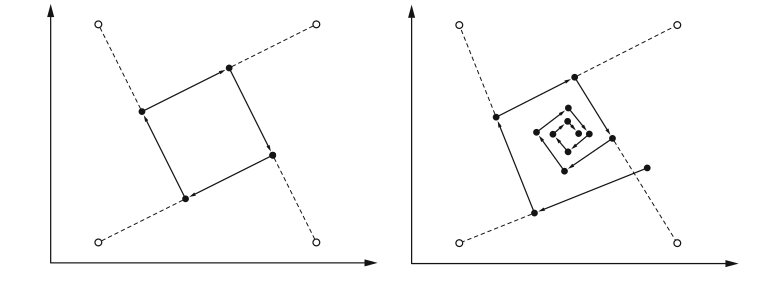
\includegraphics[scale=0.4]{img/oscill.png}
\caption{Learing rate costante (a sinistra) e decrescente (a destra).}
\label{fig:20}
\end{figure}

dove $\xi$ è un parametro specificato dall'utente e, intuitivamente, descrive l'"ampiezza" della finestra attorno al bordo delle classificazioni.
Se assumiamo che i dati siano stati scelti randomicamente da un insieme di distribuzioni normali potremmo voler usare un assegnamento \emph{soft}, in opposizione ad una divisione \emph{crisp} tipica del clustering a là c-means. Rinunciamo, quindi, alla strategia del \emph{winner-takes-all} e cerchiamo di descrivere i dati attraverso insiemi di gaussiane. In questo modo, tutti i vettori di riferimento che appartengono alla stessa classe vengono "attratti" verso il centro (con varia intensità rispetto alla distanza) e tutti quelli che non vi appartengono vengono "respinti". La densità di probabilità verrà rappresentata dalla seguente formula:

$$
f_\mathbf{X} (\mathbf{x},C) = \sum^c_{y = 1} p_Y(y,C) \cdot f_{\mathbf{X}|Y}(\mathbf{x}|y,C)
$$

dove $C$ è l'insieme dei cluster, $\mathbf{X}$ è un vettore randomico che ha come dominio lo spazio dell'input, $Y$ una variabile randomica che ha l'indice dei cluster come suo dominio, $p_Y(y,C)$ è la probabilità che un punto appartenga al $y$-esimo componente dell'insieme e $f_{\mathbf{X}|Y}(\mathbf{x}|y,C)$ è la funzione di probabilità condizionata dato il cluster $y$.
Per approssimare questa funzione, decidendo la posizione e l'ampiezza delle gaussiane, dovremo risolvere un problema di ottimizzazione comunemente chiamato \emph{maximum likelihood estimation} rispetto ai parametri del cluster. La funzione di likelihood è così calcolata:

$$
L(\mathbf{X},C) = \prod_{j=1}^n f_\mathbf{X} (\mathbf{x},C) = \prod_{j=1}^n \sum^c_{y = 1} p_Y(y,C) \cdot f_{\mathbf{X}|Y}(\mathbf{x}|y,C)
$$

Tuttavia, nella presente forma, la funzione è difficilmente ottimizzabile per via della sommatoria. Quindi, prendiamo come parametro aggiuntivo un insieme $Y_j$ di variabili:

$$
L(\mathbf{X},y,C) = \prod_{j=1}^n f_{\mathbf{X}_j,Y_j} (\mathbf{x},y_j,C)
$$

Il problema si traduce, ora, nel trovare i valori per $Y$. L'approccio utilizzato è quello di sceglierne di randomici e considerare la distribuzione di probabilità sui possibili valori. $L(\mathbf{X},y,C)$ diviene una variabile randomica di cui possiamo massimizzare il valore aspettato. Per farlo possiamo fissare $C$ in alcuni termini e computare iterativamente migliori approssimazioni.

\subsection{Self-organizing maps}

Le \emph{self-organizing maps} (o \emph{Kohonen feature maps}) sono dei feed-forward network a due layer che possono essere visti come generalizzazione dei LVQN le cui connessioni tra neuroni hidden e neuroni di output sono, però, limitate a quelle tra neuroni "vicini". Come nel caso dei LVQN, la $f_{(net)}$ dei neuroni di output è una funzione di distanza tra il vettore di input e quello dei pesi, e la $f_{(act)}$ è una funzione radiale. Una differenza rispetto ai LVQN è che la $f_{(out)}$ è la funzione identità, anche se l'output può essere reso discreto in accordo al principio del \emph{winner-takes-all}, ossia \emph{localmente} il neurone con la massima attivazione forza a 0 l'output dei neuroni circostanti. Rimane la questione di come formalizzare in modo preciso la nozione di "vicinanza" tra neuroni. Un modo per farlo è quello di costruire una struttura interna ai neuroni di output assegnando ad ogni coppia un reale che rappresenti la relazione di "vicinato"\footnote{Nel caso in cui la distanza tra neuroni è massima, di modo che la distanza tra un neurone e se stesso è 0 e quella tra neuroni diversi è infinita, avremo che la self-organizing map collassa in un LVQN.}:

$$
d_{neuroni} : U_{out} \times U_{out} \to \mathbb{R}^+
$$

\begin{figure}
\centering
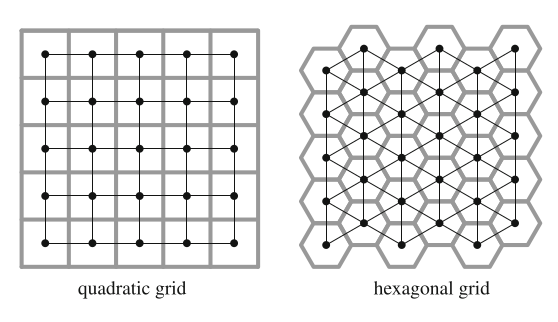
\includegraphics[scale=0.4]{img/grid.png}
\caption{Due esempi di griglie che rappresentano una relazione di vicinato tra neuroni di output: le linee scure rappresentano i neuroni più vicini, mentre quelle più chiare rappresentano le regioni in cui viene diviso lo spazio.}
\label{fig:21}
\end{figure}


Questa relazione può essere rappresentata graficamente da una griglia bidimensionale come in Figura  \ref{fig:21}. La funzione di questa rappresentazione è quella di darci un'idea anche approssimata della distanza che intercorre tra i vari vettori nello spazio di input. La self-organizing map, per tanto, costituisce una funzione che preserva la topologia, ossia una funzione che preserva la posizione relativa tra i punti del dominio. Un esempio famoso di funzione che preserva la topologia sono le così dette \emph{proiezioni di Robinson} della superficie di una sfera rispetto al piano che vengono usate per costruire le mappe del globo. Attraverso l'uso di queste funzioni la posizione relativa tra i vari punti viene conservata anche se la proporzione della distanza di due punti tra l'originale e la proiezione è più grande quanto più ci si allontana dall'equatore. Il vantaggio nell'usare queste funzioni è che ci permettono di mappare spazi multidimensionali in spazi con dimensioni minori. Come nel caso dei LVQN, il processo di apprendimento si basa sul \emph{competitive training}: ogni pattern in input viene processato ed assegnato al neurone con l'attivazione più alta. Tuttavia, a differenza di quanto accade nell'apprendimento dei LVQN non solo il neurone vincitore viene aggiornato, ma tutti i suoi vicini (sebbene in misura minore). In questo modo si ottiene che i vettori di riferimento di neuroni vicini non si muovano arbitrariamente lontani l'uno dall'altro, mantenendo così la topologia dello spazio di input. Per trovare la corretta funzione che preservi tale topologia si utilizza la seguente regola di apprendimento che costituisce una generalizzazione della attraction rule presentata nel caso dei LVQN:

$$
\mathbf{r}^{new} = \mathbf{r}^{old} + \eta(t)f_{nb}(d_{neuroni}(u,u_*),\rho(t))(\mathbf{x} - \mathbf{r}^{old})
$$

dove $u_*$ è il neurone vincitore e $f_{nb}$ è una funzione radiale. Il learning rate $\eta$ è parametrizzato rispetto al tempo perché varierà con il numero delle iterazioni. Inoltre, lo stesso raggio della funzione di vicinato in modo che si riduca progressivamente l'influenza del "centro" che è stato scelto e permetterci così una più fine approssimazione della topologia.

\subsection{Hopfield network}

Nei precedenti capitoletti ci siamo interessati esclusivamente di feed-forward network, ovvero network rappresentati da un grafo aciclico. Esistono, tuttavia, in letteratura alcuni esempi di \emph{recurrent network}, ovvero network il cui grafo contiene dei cicli diretti. Uno dei più semplici modelli di recurrent network è quello degli \emph{Hopfield network} (in quello che segue HN). Una prima differenza degli HN rispetto agli altri ANN è che tutti i neuroni sono sia neuroni di input che di output. Non esistono, inoltre, neuroni nascosti. Ogni neurone è connesso ad ogni altro neurone (sono esclusi cappi) e i pesi delle connessioni sono simmetrici. La funzione di input di ogni neurone è la somma pesata degli output degli altri neuroni:

$$
f_{(net)}^u(\ww,\ii) = \sum_{v \in U - \{u\}} w_{uv} out_v 
$$

La funzione di attivazione, invece, è una threshold function:

$$
f_{(act)}^u(net_u,\theta_u) = \begin{cases}
				1 \quad \text{se} \quad net_u >= \theta_u \\
				-1 \quad \text{se} \quad net_u < \theta_u
							  \end{cases}
$$

Mentre la funzione di output è la funzione identità. Possiamo, quindi, rappresentare un HN attraverso la sua matrice dei pesi:

$$
\mathbf{W} = \begin{bmatrix} 
			0 & w_{u_1 u_2} & \dots & w_{u_1 u_n} \\
			w_{u_2 u_1} & 0 & \dots & w_{u_2 u_n} \\
			\vdots & \vdots & \vdots & \vdots \\
			w_{u_n u_1} & w_{u_n u_2} & \dots & 0
			\end{bmatrix}
$$

Il comportamento degli HN può cambiare a seconda che i neuroni vengano aggiornati in modo sequenziale o parallelo. Se decidiamo di aggiornarli in parallelo può capitare che non si raggiunga mai uno stato stabile, ma il valore continui ad oscillare. Il teorema di convergenza ci assicura, invece, che nel caso li si aggiorni in modo sequenziale, si riesce sempre a raggiungere uno stato stabile.

\begin{theorem}
\emph{Se i neuroni di un HN sono aggiornati in modo asincrono allora uno stato stabile viene raggiunto al massimo in $n\cdot 2^n$ passi, dove $n$ è il numero dei neuroni.}
\end{theorem}

La prova del teorema si basa sul calcolo dell'energia del sistema:

$$
E = -\frac{1}{2} \sum_{u,v \in U, u \neq v} w_{uv}act_u act_v + \sum_{u \in U} \theta_u act_u
$$

Si può osservare, infatti, che il sistema può solo evolversi da uno stato con energia maggiore ad uno con energia minore. Uno stato stabile sarà un minimo locale della funzione energia. Possiamo sfruttare questo teorema per utilizzare gli HN come memorie associative, collegando un dato allo stato stabile raggiunto dopo averlo fatto processare del network. Allo stesso modo, possiamo utilizzare gli HN per calcolare problemi di ottimizzazione. Sarà sufficiente in questo caso trasformare la funzione da minimizzare in una funzione energia di un HN ed osservare gli stati stabili (aka i minimi della funzione energia) raggiunti. Per evitare di rimanere intrappolati in minimi locali è opportuno reinizializzare varie volte il network in modo randomico e ripetere gli aggiornamenti fino alla convergenza.

\subsection{Boltzmann machines}

Le macchine di Boltzmann (in quello che segue BM) possono considerarsi in tutto simili a degli HN, salvo che possono contenere neuroni nascosti e differiscono nella procedura di aggiornamento. Come nel caso degli HN, per risolvere problemi di ottimizzazione ci si basa sul fatto che è possibile definire una funzione energia associata ad ogni stato. Grazie a questa funzione energia si definisce una distribuzione di probabilità (di Boltzmann) rispetto agli stati del network:

$$
P(\mathbf{\overrightarrow{s}}) = \frac{1}{c} e^{-\frac{E(\mathbf{\overrightarrow{s}})}{kT}}
$$

dove $\mathbf{s}$ rappresenta l'insieme degli stati, $c$ è una costante di normalizzazione, $E$ è la funzione energia, $T$ è la temperatura del sistema e $k$ la costante di Boltzmann ($k \simeq 1,38 \cdot 10^{-23}$). Gli stati del sistema corrispondono ai valori che possono assumere le attivazioni dei singoli neuroni. La probabilità di attivazione di un neurone è la funzione logistica del differenziale di energia tra il caso che vede il neurone attivo e quello che lo vede inattivo.

$$
P(act_u = 1) = \frac{1}{1 + e^{-\frac{\Delta E_u}{kT}}}
$$

dove 

$$
\Delta E_u = E_{act_u = 1} - E_{act_u = 0} = \sum_{v \in U - \{u\}} w_{uv} act_v - \theta_u
$$
 
La procedura di aggiornamento chiamata \emph{Markov-chain Monte Carlo} prevede di scegliere randomicamente un neurone e calcolare il suo differenziale energetico e, con questo, la probabilità di attivazione. Questa stessa procedura  viene ripetuta varie volta fino alla convergenza del sistema. La convergenza verso uno stato stabile è garantita dal fatto che la temperatura del sistema non cresce nel tempo, ma diminuisce. Ad un certo punto si raggiungerà uno stato stabile, anche detto \emph{equilibrio termico} del sistema, che rappresenterà un minimo (possibilmente locale) della funzione.
Bisogna notare che una BM potrà calcolare in modo efficace una distribuzione di probabilità se gli esempi forniti sono compatibili con una distribuzione di Boltzmann. Per mitigare questa restrizione si dividono i neuroni di una BM tra neuroni \emph{visibili}, che ricevono i segnali di input, e \emph{nascosti}, la cui attivazione non dipende direttamente dal dataset permettendo un adattamento più flessibile ai pattern di allenamento. 

\subsubsection{Training}

L'obiettivo di apprendimento è quello di adattare i pesi e i threshold in modo che la distribuzione implicita nel dataset sia approssimata dalla distribuzione rappresentata dai neuroni visibili di una BM. Questo possiamo farlo scegliendo una misura che descriva la differenza tra le due distribuzioni ed utilizzeremo la tecnica del gradient descent per minimizzarla. Una delle misure più famose è quella di Kullback-Leibler sulla divergenza dell'informazione:

$$
KL(p1,p2) = \sum_{\omega \in \Omega} p1(\omega) ln\frac{p1(\omega)}{p2(\omega)}
$$ 

dove $p1$ si riferisce alla distribuzione del dataset e $p2$ a quella della macchina di Boltzmann. Ogni passo di apprendimento viene suddiviso in due fasi:

\begin{enumerate}
\item{\emph{Positive phase}: in cui i neuroni visibili vengono fissati rispetto ad un dato di input scelto randomicamente e i neuroni nascosti vengono aggiornati fino al raggiungimento di un equilibrio termico.}
\item{\emph{Negative phase}: tutte le unità vengono aggiornate fino al raggiungimento di uno stato stabile.}
\end{enumerate}

Se distinguiamo la probabilità che un neurone $u$ sia attivato nella positive phase ($p_u^{+}$) e quella che lo stesso neurone sia attivato nella negative phase ($p_u^{-}$) e la probabilità che due neuroni $u$ e $v$ siano attivati simultaneamente nella positive phase ($p_{uv}^{+}$) e quella che gli stessi due neuroni siano attivati nella negative phase ($p_{uv}^{-}$), possiamo definire la regola di update dei pesi e del threshold come segue:

$$
\Delta w_{uv} = \frac{1}{\eta} (p_{uv}^{+} - p_{uv}^{-}) 
\quad
\text{e}
\quad
\Delta \theta_u = -\frac{1}{\eta}(p_u^{+} - p_u^{-})
$$
 
Intuitivamente: se lo stesso neurone viene sempre attivato ogniqualvolta viene presentato lo stesso input allora il suo threshold dovrà essere ridotto. Allo stesso modo, se due neuroni vengono spesso attivati assieme allora il peso che corrisponde alla loro connessione verrà aumentato (“cells that fire together, wire together”).

\subsubsection{Restricted Boltzmann machines}

 Sebbene le BM siano molto potenti, allenarne anche di medie dimensioni è molto dispendioso. Per questo sono state introdotte le \emph{restricted Boltzmann machines} (in quello che segue RBM). La differenza rispetto alle normali BM è che il grafo del network di un RBM è un grafo bipartito, ovvero una connessione è possibile solo tra neuroni di gruppi differenti. Solitamente uno dei gruppi è formato dai neuroni visibili e l'altro da quelli nascosti. Un vantaggio di avere un network in cui non vi sono connessioni tra neuroni dello stesso gruppo è che il processo di apprendimento può essere compiuto ripetendo questi tre passi:
\begin{enumerate}
\item{Fase I: le unità di input vengono fissate rispetto ad un pattern scelto casualmente e quelle nascoste vengono aggiornate in parallelo ottenendo quello che si chiama in gergo \emph{positive gradient}.}
\item{Fase II: avendo ottenuto un input preprocessato nella prima fase, si invertono le parti e si fissano i neuroni nascosti e si aggiornano quelli visibili, ottenendo così il \emph{negative gradient}.}
\item{Fase III: si aggiornano pesi e threshold con la differenza tra positive e negative gradient.}
\end{enumerate}
In letteratura le RBM sono state utilizzate per costruire con più layer in modo simile a quanto accade con gli autoencoder nei MLP.
 
\subsection{Recurrent network}

Sia gli HN che le BM sono esempi di \emph{recurrent network}, ovvero network il cui grafo ha al suo interno dei cicli. L'output in questi network viene generato solo se viene raggiunto uno stato stabile nella computazione. L'evoluzione di questi sistemi può essere descritta attraverso l'utilizzo di equazioni differenziali. Dato, infatti, un insieme alcune equazioni differenziali rappresentate in forma ricorsiva:

$$
x(t_i) = x(t_{i-1}) + \Delta y_1(t_{i-1})
$$
$$
y_1(t_i) = y_1(t_{i-1}) + \Delta y_2(t_{i-1})
$$
$$
\vdots
$$
$$
y_{i-1}(t_i) = y_{i-1}(t_{i-1}) + f(t_{i-1}, x(t_{i-1}), \dots, y_{n-1}(t_{i-1}))
$$

possiamo sfruttare la derivata della funzione nell'istante di tempo precedente per calcolare il valore successivo. Questo permette di trasformarle in un recurrent network, creando per ogni variabile un nodo nel grafo e associando alle connessioni il valore del differenziale come in Figura \ref{fig:22}.

\begin{figure}
\centering
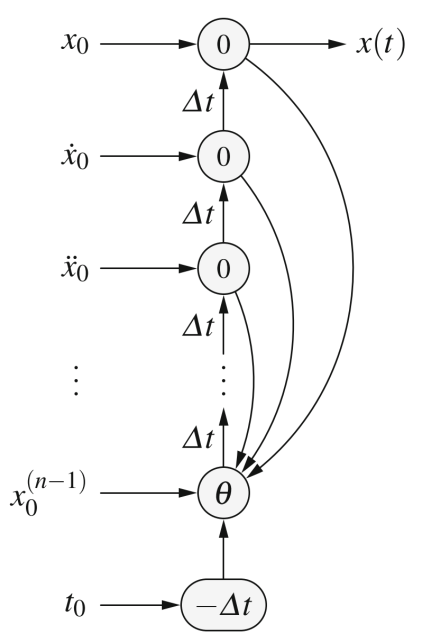
\includegraphics[scale=0.3]{img/recurrent.png}
\caption{Recurrent network.}
\label{fig:22}
\end{figure}

Possiamo generalizzare questo approccio a funzioni con più di un argomento grazie ai \emph{vectorial neural network}. Se, tuttavia, non conosciamo in precedenza la struttura della computazione non possiamo sfruttare la backpropagation così come l'abbiamo presentata, in quanto gli errori si propagano senza soluzione di continuità lungo i cicli del network. Un modo per risolvere questo problema è quello di dispiegare nel tempo la computazione ogni qualvolta questa attraversi un ciclo e aggiungere una copia dei neuroni così attraversati come un layer addizionale. A questo punto si potrà applicare la backpropagation come in un qualsiasi feed-forward network. Per calcolare gli aggiornamenti ai pesi e ai threshold sarà, però, necessario combinare gli aggiustamenti calcolati rispetto ai neuroni così aggiunti. 
 
\section{Sistemi fuzzy}

\subsection{Introduzione alla logica fuzzy}

\subsubsection{Motivazioni}

La logica classica si fonda sul \emph{principio di bivalenza}, ovvero una proposizione può assumere solo due valori di verità: il \emph{vero} o il \emph{falso}. Questa assunzione può essere adeguata nel caso in cui ci interessi modellare concetti chiari e distinti che hanno definizioni precise, come nel caso dei concetti matematici. Quando, invece, vogliamo formalizzare la conoscenza implicita nel linguaggio naturale possiamo imbatterci in alcune proposizioni che sono vere (o false) \emph{in una certa misura}, oppure proprietà che hanno estensioni sfumate. La logica fuzzy e la teoria insiemistica che da questa discende ci permette di ragionare in questi contesti, in modo da sfruttare a nostro vantaggio la vaghezza insita nell'uso che facciamo delle parole nel linguaggio naturale. Bisogna, tuttavia, stare attenti a non confondere l'imprecisione con l'\emph{incertezza}. L'incertezza si riferisce alla possibilità che un evento accada o meno. Il valore numerico associato all'accadimento di un evento incerto si chiama \emph{probabilità} ed è studiato dalla branca della matematica omonima. La differenza tra appartenenza fuzzy e probabilità sta nel fatto che la probabilità rimane comunque un fenomeno booleano: un evento può accadere o non accadere; dove, invece, l'appartenenza fuzzy si riferisce a quanto una proprietà viene soddisfatta da un oggetto. 

\subsubsection{Insiemi fuzzy}

Un insieme classico è una collezione di elementi che possono (o meno) appartenere all'insieme. Per tanto, un insieme può essere definito a partire da una funzione caratteristica che assegna ad ogni elemento nel dominio del discorso il valore 1 se questo elemento appartiene all'insieme oppure 0 altrimenti. Un 	\emph{insieme fuzzy} può essere visto come una generalizzazione di questo concetto.
\begin{definition}
 Dato un dominio del discorso $X$, un insieme fuzzy $\mu$ è una funzione $\mu : X \to [0,1]$ che assegna ad ogni elemento un \emph{grado di appartenenza} $\mu(x)$ rispetto all'insieme $\mu$.
\end{definition}
 Queste funzioni sono scelte a seconda del contesto di utilizzo e i gradi di appartenenza sono fissati per convenzione. Possiamo vedere i fuzzy set come interfacce tra espressioni linguistiche e loro rappresentazioni numeriche. Ad esempio, vogliamo dare un modello formale alla proprietà "essere alto per un bambino di 4 anni". Per farlo definiremo un insieme fuzzy $\mu_{tall}$ attraverso una funzione sigmoide come in Figura \ref{fig:23}, tale per cui risulteranno \emph{sicuramente} nell'estensione della proprietà i bambini più alti di 1.5 m centimetri e \emph{sicuramente} fuori dall'estensione quelli più bassi di 0.7 m. Tutti gli altri apparterranno all'insieme con un certo grado.

\begin{figure}
\centering
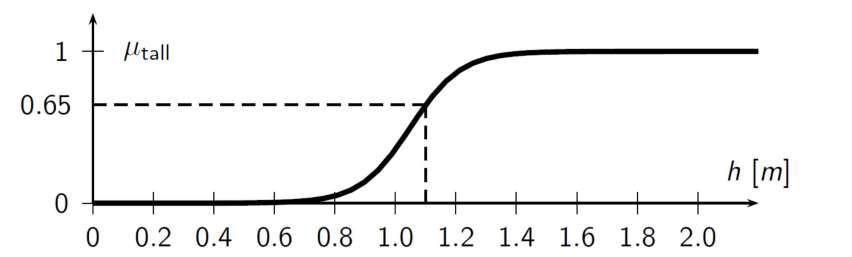
\includegraphics[scale=0.3]{img/tall.png}
\caption{L'insieme fuzzy $\mu_{tall}$ che descrive il predicato "essere alto per un bambino di 4 anni".}
\label{fig:23}
\end{figure}

\subsubsection{Interpretazioni della funzione di appartenenza}

Ci sono varie semantiche che è possibile associare alla relazione di appartenenza fuzzy a seconda dell'applicazione:

\begin{enumerate}
\item{somiglianza}
\item{preferenza}
\item{possibilità}
\end{enumerate}

Nel primo caso, $\mu(x)$ può essere visto come il grado di prossimità rispetto ad un elemento prototipale di $\mu$. Questa interpretazione viene utilizzata nei problemi di pattern classification, cluster analysis e regressione. Nel secondo caso, la funzione $\mu$ rappresenta sia l'insieme degli oggetti preferiti, sia il valore associato ad una decisione $X$ e $\mu(u)$ rappresenta sia l'intensità della preferenza associata a $u$, sia la possibilità di scegliere $u$ come valore di $X$. Questa interpretazione viene utilizzata nei problemi di ottimizzazione fuzzy e nella teoria della decisione. L'ultima delle tre è quella che considera $\mu(u)$ come il grado di possibilità che l'elemento $u$ sia il valore del parametro $X$ ed è usata per quantificare lo stato epistemico di un agente. L'obiettivo è quello di distinguere quello che l'agente considererebbe "sorprendente" da quello che, invece, è "tipico" o "aspettato". Questa interpretazione, come vedremo in seguito, viene utilizzata in data analysis.

\subsubsection{Rappresentazione verticale e orizzontale}

Come abbiamo già mostrato, gli insiemi fuzzy possono essere rappresentati da una funzione che assegna un valore nell'intervallo reale unitario ad ogni elemento dell'universo del discorso. Nella maggior parte delle applicazioni i valori assunti dalla funzione crescono monotonicamente fino a un certo punto e da quello decrescono monotonicamente. Questo tipo di insiemi viene detto \emph{convesso}. Le funzioni che rappresentano insiemi convessi sono dette \emph{funzioni triangolari} ed assumono la forma:

$$
\Lambda_{a,b,c} : \mathbb{R} \to [0,1],\quad x \mapsto 
\begin{cases}
\frac{x-a}{b-a} \text{ if } a \leq x < b \\
\frac{c-x}{c-b} \text{ if } b \leq x \leq c \\
0 \quad \text{  altrimenti}
\end{cases}
$$

Le funzioni triangolari possono essere considerate un caso particolare delle \emph{funzioni trapezoidali}:

$$
\Pi_{a,b,c,d} : \mathbb{R} \to [0,1],\quad x \mapsto 
\begin{cases}
\frac{x-a}{b-a} \text{ if } a \leq x \leq b \\
1 \quad \text{ if  }  b \leq x \leq c \\
\frac{d-x}{d-c} \text{ if } c \leq x \leq d \\
0 \quad \text{  altrimenti}
\end{cases}
$$

\begin{figure}
\centering
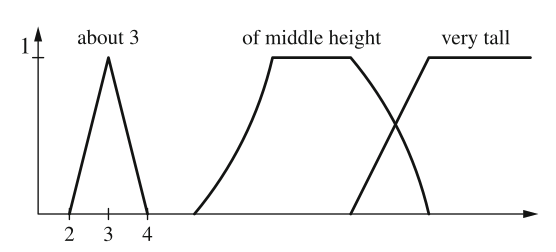
\includegraphics[scale=0.4]{img/triang.png}
\caption{Alcuni esempi di funzioni triangolari e trapezoidali.}
\label{fig:24}
\end{figure}

Alcuni esempi di queste funzioni possono essere trovati in Figura \ref{fig:24}. Questa rappresentazione dei fuzzy set viene anche detto \emph{rappresentazione verticale}. Una diversa rappresentazione è invece quella \emph{orizzontale}. Per un qualsiasi valore $\alpha \in [0,1]$ consideriamo l'insieme di elementi che hanno un grado di appartenenza all'insieme $\mu$ di almeno $\alpha$.

\begin{definition}
Sia $\mu$ un fuzzy set definito rispetto al dominio del discorso $X$ e sia $\alpha \in [0,1]$. L'insieme
$$
[\mu]_\alpha = \{x \in X | \mu(x) \geq \alpha \}
$$
è chiamato \emph{alpha-cut} dell'insieme $\mu$.
\end{definition}

Nel caso in cui l'insieme $\mu$ sia una funzione trapezoidale, qualsiasi suo alpha-cut sarà un intervallo chiuso. Se, invece, l'insieme non è convesso almeno uno dei suoi alpha-cut consisterà in due intervalli disgiunti. Alcune proprietà degli alpha-cut sono le seguenti:

\begin{enumerate}
\item{$[\mu]_0 = X$}
\item{$\alpha \leq \beta \implies [\mu]_\alpha \subseteq [\mu]_\beta $}
\item{$\cap_\alpha: \alpha < \beta, [\mu]_\alpha = [\mu]_\beta$}
\end{enumerate} 

Da queste proprietà discende il fatto che ogni insieme fuzzy possa essere descritto specificando una famiglia di alpha-cut, come illustra il teorema seguente.

\begin{theorem}
Sia $\mu$ un fuzzy set, allora
$$
\mu(x) = \sup_{\alpha \in [0,1]} \{x \in [\mu]_\alpha\}
$$
\end{theorem}

\begin{figure}
\centering
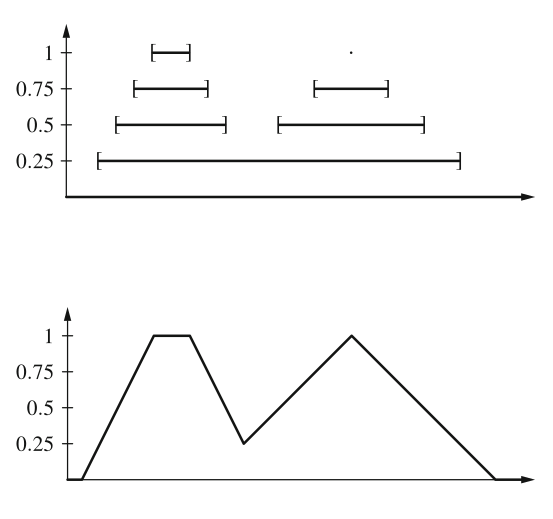
\includegraphics[scale=0.3]{img/alpha_cut.png}
\caption{Insieme fuzzy e sua rappresentazione in termini di alpha-cut.}
\label{fig:25}
\end{figure}

Dal punto di vista geometrico, un fuzzy set può essere visto come un inviluppo superiore dei suoi alpha-cut. Questa connessione tra insiemi fuzzy e famiglie di alpha-cut è utilizzata nella rappresentazione degli insiemi fuzzy nei computer. Solitamente ci si limita a prendere un numero di finito di alpha-cut rilevanti ai fini della rappresentazione dell'insieme(Figura \ref{fig:25}). Gli insiemi vengono poi conservati in memoria come catene di liste lineari. Ogni lista è l'unione di intervalli rappresentati dai loro estremi. 

\subsubsection{Alcune utili definizioni}

Avendo introdotto gli alpha-cut come uno strumento per rappresentare i fuzzy set, ora li sfrutteremo definendo alcuni concetti molto utili per quello che segue.

\begin{definition}
Il \emph{supporto} $S(\mu)$ di un insieme fuzzy $\mu$ è l'insieme booleano che contiene tutti e soli gli elementi del dominio del discorso che hanno un grado di appartenenza non nullo rispetto a $\mu$. In simboli:
$$
S(\mu) = [\mu]_{\bar{0}} = \{ x \in X | \mu(x) > 0 \}
$$
\end{definition}

\begin{definition}
Il \emph{centro} $C(\mu)$ di un insieme fuzzy $\mu$ è l'insieme booleano che contiene tutti e soli gli elementi del dominio del discorso che hanno un grado di appartenenza uguale a 1 rispetto a $\mu$. In simboli:
$$
C(\mu) = [\mu]_{1} = \{ x \in X | \mu(x) = 1 \}
$$
\end{definition}

\begin{definition}
L'\emph{altezza} $h(\mu)$ di un insieme fuzzy $\mu$ è il più alto grado di appartenenza ottenibile da un elemento di $\mu$. In simboli:
$$
h(\mu) = \sup_{x \in X} \{\mu(x)\}
$$
\end{definition}

\begin{definition}
Un insieme fuzzy $\mu$ è definito \emph{normale} sse $h(\mu) = 1$. Altrimenti, è definito \emph{subnormale}.
\end{definition}

\begin{definition}
Un insieme fuzzy $\mu$ è definito \emph{convesso} sse i suoi alpha-cut sono convessi per ogni scelta di $\alpha \in [0,1)$.
\end{definition}

\begin{definition}
Un insieme fuzzy $\mu$ è un \emph{numero fuzzy} sse $\mu$ è normale e $[\mu]_\alpha$ è chiusa, limitata e convessa per ogni scelta di $\alpha \in [0,1)$.
\end{definition}

\subsubsection{Logica fuzzy}

Un importante risultato della logica classica dice che esiste un isomorfismo tra la logica proposizione su un insieme finito di variabili e la teoria degli insiemi finiti. Entrambi questi sistemi, inoltre, possono essere dimostrati isomorfi ad un'algebra booleana finita. Questo ci permette di definire gli operatori insiemistici utilizzando i classici operatori logici di congiunzione, disgiunzione e negazione. Un discorso simile vale per la logica fuzzy, ovvero la logica che ha come insieme di valori di verità l'intero intervallo reale $[0,1]$. Una volta ridefiniti gli operatori logici booleani per adattarsi alla nuova semantica potremo usarli per costruirci sopra una teoria degli operatori insiemistici "fuzzy". Siano $\mu$ e $\mu'$, possiamo definire gli operatori della logica fuzzy come segue:
\begin{enumerate}
\item{$\neg \mu \doteq 1 - \mu(x)$} 
\item{$\mu \wedge \mu' \doteq \min\{\mu(x),\mu'(x)\}$}
\item{$\mu \vee \mu' \doteq \max\{\mu(x),\mu'(x)\}$}
\end{enumerate}

\begin{figure}
\centering
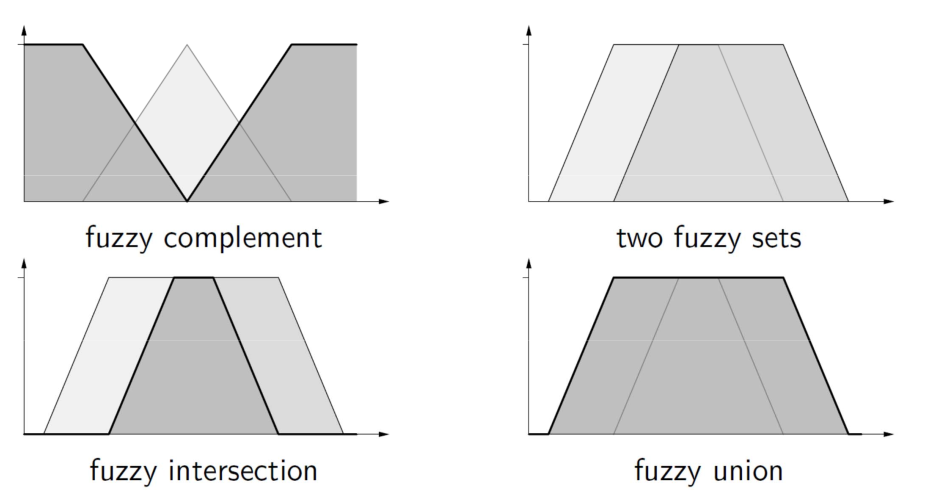
\includegraphics[scale=0.3]{img/fuzzyop.png}
\caption{Le varie operazioni insiemistiche caratterizzate secondo le definizioni riportate nella sezione 3.1.6.}
\label{fig:26}
\end{figure}

Gli operatori insiemistici associati sono mostrati in Figura \ref{fig:26}.

\subsubsection{Negazione stretta e forte}

In generale, esistono vari modi di definire la negazione in una logica fuzzy. L'unico requisito è che la definizione rispetti tre proprietà che, intuitivamente, ogni negazione deve possedere:

\begin{enumerate}
\item{$\neg(0) = 1$} 
\item{$\neg(1) = 0$}
\item{$x \leq y \implies \neg x \geq \neg y$}
\end{enumerate}

In aggiunta a queste proprietà, una negazione può soddisfarne altre. Per esempio, si può chiedere che sia \emph{strettamente decrescente}:

$$
x < y \implies \neg x > \neg y
$$

Oppure che $\neg$ sia \emph{continua}, o \emph{involutiva}:

$$
\neg \neg x = x
$$

\begin{definition}
Una negazione si dice \emph{stretta} sse è strettamente decrescente e continua.
\end{definition}

\begin{definition}
Una negazione si dice \emph{forte} sse è stretta e involutiva.
\end{definition}

\subsubsection{T-norme e t-conorme}

Come la negazione, la congiunzione e la disgiunzione fuzzy possono essere definite in diversi modi. Entrambe devono, tuttavia, soddisfare alcune proprietà di base che le definiscono rispettivamente come \emph{t-norme} e \emph{t-conorme}.

\begin{definition}
Una funzione $\top : [0,1]^2 \to [0,1]$ si dice \emph{t-norma} sse soddisfa le seguenti proprietà:
\begin{enumerate}
\item{$\top(x,1) = x$}
\item{$\top(x,y) = \top(y,x)$}
\item{$\top(x,\top(y,z)) = \top(\top(x,y),z)$}
\item{$x \leq z \implies \top(x,y) \leq \top(x,z)$}
\end{enumerate}
\end{definition}

\begin{definition}
Una funzione $\bot: [0,1]^2 \to [0,1]$ si dice \emph{t-conorma} sse soddisfa le seguenti proprietà:
\begin{enumerate}
\item{$\bot(x,0) = x$}
\item{$\bot(x,y) = \bot(y,x)$}
\item{$\bot(x,\bot(y,z)) = \bot(\bot(x,y),z)$}
\item{$x \leq z \implies \bot(x,y) \leq \bot(x,z)$}
\end{enumerate}
\end{definition}

Le definizioni di disgiunzione e congiunzione che abbiamo dato nella sezione 3.1.6 in termini di $\max$ e $\min$ soddisfano queste proprietà. Si può mostrare che l'operazione di minimo sia la più grande t-norma e il massimo la più piccola t-conorma. In aggiunta a queste, possono essere date altre definizioni di disgiunzione e congiunzione come, per esempio, quella in termini di prodotto e somma probabilistica:
$$
\top_{prod}(x,y) = x \cdot y
$$
$$
\bot_{sum} (x,y) = x + y - x \cdot y
$$

Oppure, seguendo Łukasiewicz:
$$
\top_{Luk}(x,y) = \max\{0,x + y - 1\}
$$
$$
\bot_{Luk}(x,y) = \min\{1,x + y\}
$$
O ancora, come prodotto e somma drastica:
$$
\top_{-1}(x,y) = \begin{cases}
				\min(x,y) \quad \text{se } \max(x+y) = 1 \\
				0 \quad \text{ altrimenti}  
				\end{cases}
$$
$$
\bot_{-1}(x,y) = \begin{cases}
				\max(x,y) \quad \text{se } \min(x+y) = 0 \\
				0 \quad \text{ altrimenti}  
				\end{cases}
$$

\begin{figure}
\centering
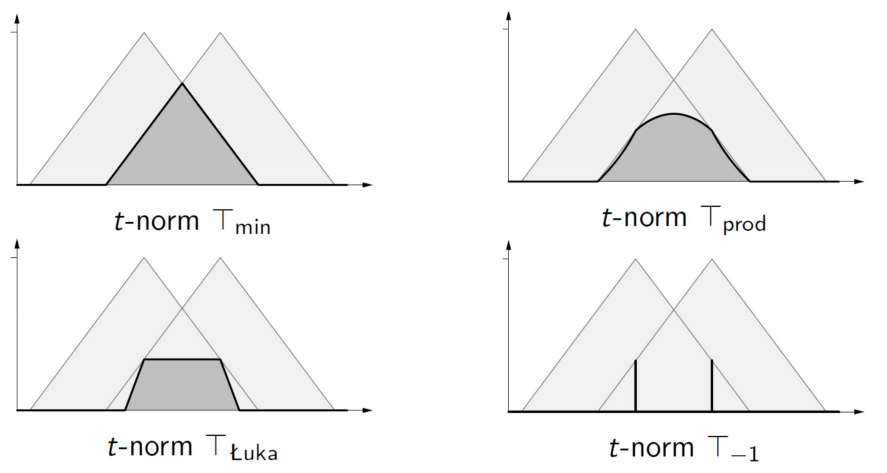
\includegraphics[scale=0.3]{img/tnorme.png}
\caption{Alcune definizioni di t-norme.}
\label{fig:27}
\end{figure}

In Figura \ref{fig:27} si possono vedere le relazioni che legano tutte le precedenti definizioni di t-norma. In Figura \ref{fig:28}, invece, si possono vedere le varie t-conorme.

\begin{figure}
\centering
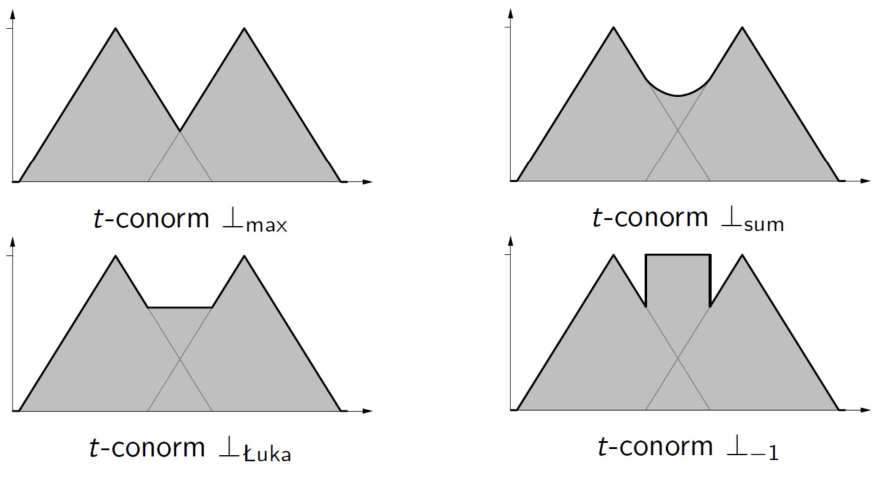
\includegraphics[scale=0.3]{img/tconorme.png}
\caption{Alcune definizioni di t-conorme.}
\label{fig:28}
\end{figure}

\subsubsection{Implicazione fuzzy}

Come nel caso booleano avremo che un insieme fuzzy è contenuto in un altro se tutti gli elementi del primo sono contenuti nel secondo. Sfruttando l'isomorfismo tra operatori logici e insiemistici, inoltre potremo definire il concetto di sottoinsieme a partire da quello di implicazione come segue:
$$
I(a,b) = \neg a \vee b
$$
A seconda della semantica che daremo ai nostri operatori logici fuzzy avremo varie classi di implicazioni. 

\begin{enumerate}
\item{\emph{S-implication}: $I(a,b) = \bot(\neg a, b)$}
\item{\emph{R-implication}: $I(a,b) = \sup \{x \in [0,1] | \top(a,x) \leq b\}$}
\item{\emph{QL-implication}: $I(a,b) = \bot(\neg a, \top(a,b))$}
\end{enumerate}

\subsection{Teoria della logica fuzzy}

\subsubsection{Principio di estensione}

Come estendere una funzione $\phi : X^n \to Y$ in un contesto fuzzy di modo che $\hat{\phi}$ abbia come dominio una tupla di fuzzy set e come codominio un fuzzy set? Un caso particolare è quello della valutazione di proposizioni. Definito un assegnamento fuzzy alle proposizioni atomiche, possiamo estenderlo a combinazioni arbitrarie di formule legate tra loro da operatori logici (and e or):
$$
truth: \mathbb{P} \to [0,1]
$$
$$
truth(a\text{ and }b) =  \min\{truth(a),truth(b)\}
$$
$$
truth(a\text{ or }b) =  \max\{truth(a),truth(b)\}
$$
Si possono considerare anche congiunzioni e disgiunzioni infinite:
$$
truth(\forall i \in I : a_i) = 	\inf \{ truth(a_i) | i \in I \}
$$
$$
truth(\exists i \in I : a_i) = 	\sup \{ truth(a_i) | i \in I \}
$$
Questo ci permemette di riguadagnare la logica booleana anche nel caso fuzzy. Un altro esempio di estensione è quella della somma reale tra insiemi definita, per insiemi classici, come:
$$
+ : 2^{\mathbb{R}} \times 2^{\mathbb{R}} \to 2^{\mathbb{R}}
$$
$$
(A,B) \to A + B = \{y | \exists a,b (y = a + b) \land (a \in A) \land (b \in B) \}
$$
La sua estensione ai fuzzy set verrà definita per $\mu$ e $\mu'$ fuzzy set come:
$$
(\mu,\mu') \to \mu \oplus \mu' 
$$
$$
truth(y \in \mu \oplus \mu') = \sup_{a,b}\{ truth(y = a + b) \land truth(a \in A) \land truth(b \in B)\}
$$
$$
= \sup_{a,b:y=a+b} \{ \min(\mu(a),\mu'(b)) \}
$$
In generale, una funzione $\phi : X^n \to Y$ può essere estesa ad una $\hat{\phi} : [2^X]^n \to 2^Y$ su insiemi classici nel seguente modo:
$$
\hat{\phi} (A_1, \dots, A_n) = \{ y \in Y | \exists x_1, \dots, x_n \in A_1 \times \dots \times A_n : \phi(x_1,\dots,x_n) = y \}
$$
Basandoci su questa definizione possiamo poi generalizzare al caso dei fuzzy set su un dominio di discorso $X$:
$$
\hat{\phi}_{fuzzy} (\mu_1, \dots, \mu_n) = \sup\{ \min \{ \mu_1(x_1), \dots, \mu_n(x_n) \} | (x_1, \dots, x_n) \in X^n \land \phi(x_1, \dots, x_n) = y \}
$$
Assumendo che $\sup \emptyset = 0$.

\subsubsection{Alcuni insiemi fuzzy rilevanti}

Vi sono vari tipi di insiemi fuzzy. Per quanto ci riguarda particolare rilevanza assumono quelli definiti sull'insieme $\mathbb{R}$. Un insieme fuzzy sui reali ha un significato quantitativo che può essere utilizzato per rappresentare variabili fuzzy. Queste ultime giocano un ruolo importantissimo in molte applicazioni: fuzzy control, ragionamento approssimato, ottimizzazione, etc. Alcune classi di $F(\mathbb{R})$ (l'insieme degli insiemi fuzzy sui reali) che vengono citate spesso in letteratura sono le seguenti:
\begin{enumerate}
\item{Normal fuzzy set: \\ $F_N(\mathbb{R}) = \{\mu \in F(\mathbb{R}) | \exists x \in \mathbb{R} : \mu(x) = 1 \}$}
\item{Upper Semi-continuous fuzzy set: \\$F_C(\mathbb{R}) = \{\mu \in F_N(\mathbb{R}) | \forall \alpha \in (0,1] : [\mu]_\alpha \text{ è compatto }\}$}
\item{Fuzzy interval: \\ $F_I(\mathbb{R}) = \{\mu \in F_N(\mathbb{R}) | \forall a,b,c \in \mathbb{R} : c \in [a,b] \implies \mu(c) \geq \min\{ \mu(a),\mu(b) \} \}$}
\end{enumerate}

\begin{figure}
\centering
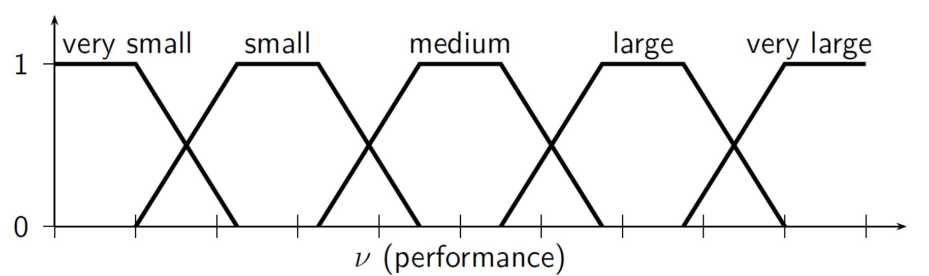
\includegraphics[scale=0.3]{img/lingvar.png}
\caption{Esempio di variabile linguistica.}
\label{fig:29}
\end{figure}

Particolare interesse rivestono i fuzzy interval anche detti \emph{fuzzy numbers} perché permettono di definire \emph{variabili fuzzy quantitative}. Tali variabili assumono come valore numeri fuzzy. Quando le quantità fuzzy rappresentano concetti linguistici (come piccolo, grande, etc.) si parla di variabili linguistiche (vedi Figura \ref{fig:30}). Ogni variabile linguistica è definita da un quintupla $(v,T,X,g,m)$, dove $v$ è il nome della variabile, $T$ è l'insieme dei termini che coprono $v$, $X$ è il dominio del discorso, $g$ è la grammatica per generare i termini ed $m$ la semantica che assegna ad ogni termine un fuzzy number. Per processare questo genere di variabili occorrerà estendere le operazioni insiemistiche e aritmetiche originalmente utilizzate per i numeri. 

\subsubsection{Rappresentazione per insiemi}

Abbiamo visto in precedenza come, attraverso il principio di estensione, si possano definire le operazioni aritmetiche nel contesto di $F(\mathbb{R})$. Tuttavia, calcolare tali funzioni direttamente sugli insiemi fuzzy risulta oneroso, specialmente se si adotta la rappresentazione verticale rispetto a quella orizzontale. Sarebbe desiderabile ridurre l'aritmetica fuzzy all'ordinaria aritmetica sugli insiemi booleani e, quindi, applicare alcune semplici operazioni su intervalli per ottenere il risultato. Questo è possibile farlo attraverso la \emph{rappresentazione per insiemi} di un insieme fuzzy.

\newpage

\begin{definition}
Una famiglia $(A_\alpha)_{\alpha \in (0,1)}$ è una \emph{rappresentazione per insiemi} di $\mu \in F_N(\mathbb{R})$ se
\begin{enumerate}
\item{$0 < \alpha < \beta < 1 \implies A_\alpha \subseteq A_\beta \subseteq \mathbb{R}$}
\item{$\mu(t) = \sup \{ \alpha \in [0,1] | t \in A_\alpha \} $}
\end{enumerate} 
\end{definition}

Il seguente teorema ci assicura che una rappresentazione per insiemi è una fedele immagine dell'insieme fuzzy che raffigura.

\begin{theorem}
Sia $\mu \in F_N(\mathbb{R})$. La famiglia $(A_\alpha)_{\alpha \in (0,1)}$ è una rappresentazione per insiemi di $\mu$ sse 
$$
[\mu]_{\bar{\alpha}} = \{ t \in \mathbb{R} | \mu(t) > \alpha \} \subseteq A_\alpha \subseteq \{ t \in \mathbb{R} | \mu(t) \geq \alpha \} = [\mu]_\alpha
$$
è valida per ogni $\alpha \in (0,1)$.
\end{theorem}

Se $\mu_1, \dots, \mu_n$ sono normal fuzzy set su $\mathbb{R}$ e $\phi: \mathbb{R}^n \to \mathbb{R}$ una funzione e $\hat{\phi}$ la sua estensione fuzzy. Allora valgono le seguenti:

$$
\forall \alpha \in [0,1) : [\hat{\phi}(\mu_1,\dots,\mu_n)]_{\bar{\alpha}} = \phi([\mu_1]_{\bar{\alpha}}, \dots, [\mu_n]_{\bar{\alpha}})
$$
$$
\forall \alpha \in [0,1) : [\hat{\phi}(\mu_1,\dots,\mu_n)]_\alpha \subseteq \phi([\mu_1]_\alpha, \dots, [\mu_n]_\alpha)
$$

Sia, quindi, $(A_\alpha)_{\alpha \in (0,1)}$ la rappresentazione per insiemi di $\mu_i$ per $1 \geq i \geq n$, allora $(\phi((A_1)_\alpha, \dots, (A_n)_\alpha))_{\alpha \in (0,1)}$ è una rappresentazione di $\hat{\phi}$. 

\subsubsection{Relazioni fuzzy}

Una relazione booleana $R$ tra gli insiemi $X_1, \dots, X_n$ è un sottoinsieme del loro prodotto cartesiano. Ogni relazione di questo tipo può essere definita, quindi, attraverso la propria funzione caratteristica:
$$
R(x_1,\dots,x_n) = \begin{cases}
						1 \text{ se e solo se } (x_1, \dots, x_n) \in R \\
						0 \text{ altrimenti }
					\end{cases}
$$

Come accade nel caso della funzione caratteristica di insiemi, quella delle relazioni può essere generalizzata per comprendere valori fuzzy. Il grado di appartenenza indica la forza della relazione tra i membri della tupla in considerazione. Siano $n \geq 2$ fuzzy set $A_1, \dots, A_n$ definiti rispettivamente sul dominio del discorso $X_1, \dots, X_n$. Il prodotto cartesiano $A_1 \times \dots \times A_n$ è una relazione fuzzy nello spazio prodotto $X_1 \times \dots \times X_n$ ed è definita dalla seguente funzione di partecipazione:
$$
\mu_{A_1 \times \dots \times A_n}(x_1, \dots, x_n) = \top(\mu_{A_1}(x_1), \dots,\mu_{A_n}(x_n))
$$	 
Dove $\top$ è una t-norma, solitamente il minimo o il prodotto.

\begin{definition}
Siano $\ww = (x_1, \dots, x_n)$ e $\vv = (y_1, \dots, y_m)$ due tuple. $\ww$ è chiamato \emph{sottosequenza} di $\vv$ (in simboli, $\ww \prec \vv$) sse $\forall j \in \{1,\dots,n\}, \ww_j = \vv_j$.
\end{definition}

\begin{definition}
Data un relazione $R(x_1,\dots,x_n)$ e un sottoinsieme dei domini del discorso $Y \subseteq \{X_1, \dots, X_n\}$, denotiamo con $[R \downarrow Y]$ la \emph{proiezione} di $R$ su $Y$ definita come:
$$
[R \downarrow Y](\vv) = \max_{\vv \prec \ww} R(\ww)
$$
\end{definition}

\begin{definition}
Data una proiezione $[R \downarrow Y]$, una \emph{estensione cilindrica} che denotiamo come $[R \uparrow X-Y]$ è la relazione $R$ di partenza salvo che ogni valore diverso da quello della proiezione viene sosituito con quello stesso valore:
$$
[R \uparrow X-Y](\vv) = R(\ww)
$$
\end{definition}

\subsubsection{Relazioni binarie}

Le relazioni binarie sono esempi particolarmente rilevanti tra tutte le relazioni $n$-dimensionali, in quanto generalizzazioni delle funzioni matematiche. Contrariamente a ciò che accade nel caso delle funzioni da $X$ a $Y$, una relazione $R(X,Y)$ può assegnare ad un elemento di $X$ ad un valore in $Y$. Possiamo estendere le consuete operazioni sulle funzioni (inversa e composizione) anche alle relazioni fuzzy. 

\begin{definition}
Data una relazione $R(X,Y)$ il suo \emph{dominio}, denotato $dom R$, è definito come:
$$
dom R(x) = \max_{y \in Y}\{ R(x,y) \}
$$
\end{definition}

\begin{definition}
Data una relazione $R(X,Y)$ il suo \emph{codominio}, denotato $ran R$, è definito come:
$$
ran R(x) = \max_{x \in X}\{ R(x,y) \}
$$
\end{definition}

\begin{definition}
Data una relazione $R(X,Y)$ la sua \emph{altezza}, denotata $h R$, è definito come:
$$
h R(x) = \max_{x \in X} \max_{y \in Y} \{ R(x,y) \}
$$
\end{definition}

\begin{definition}
Data una relazione $R(X,Y)$ la sua \emph{inversa}, denotata $R^{-1}$, è definito come quella relazione su $Y \times X$ tale che:
$$
R^{-1} (y,x) = R(x,y) \quad \forall x \in X, \forall y \in Y
$$
\end{definition}

\begin{definition}
Data una relazione $R(X,Y)$ e una relazione $Q(Y,Z)$ la loro \emph{composta}, denotata $R \circ Q (X,Z)$, è definito come quella relazione su $X \times Z$ tale che:
$$
R \circ Q (x,z) = \sup_{y \in Y} \{ \min \{ P(x,y),Q(y,z)\} \quad \forall x \in X, \forall z \in Z \} 
$$
\end{definition}

\begin{definition}
Data una relazione $R(X,Y)$ e una relazione $Q(Y,Z)$ il loro \emph{join}, denotata $R \star Q (X,Y,Z)$, è definito come quella relazione su $X \times Y \times Z$ tale che:
$$
R \star Q (x,y,z) = \min \{ P(x,y),Q(y,z)\} \quad \forall x \in X, \forall y \in Y, \forall z \in Z 
$$
\end{definition}

\begin{definition}
Data una relazione $R(X,X)$ si definisce una \emph{relazione di equivalenza} sse soddisfa le seguenti proprietà:
\begin{enumerate}
\item{\emph{riflessività}: $\forall x \in X \quad R(x,x) = 1$ }
\item{\emph{simmetria}: $\forall x,y \in X \quad R(x,y) = R(y,x)$ }
\item{\emph{transitività}: $\forall (x,z) \in X^2 \quad R(x,z) \geq \max_{y \in X} \min \{ R(x,y),R(y,z) \}$ }
\end{enumerate}
\end{definition}

\subsection{Fuzzy controller}

\begin{figure}
\centering
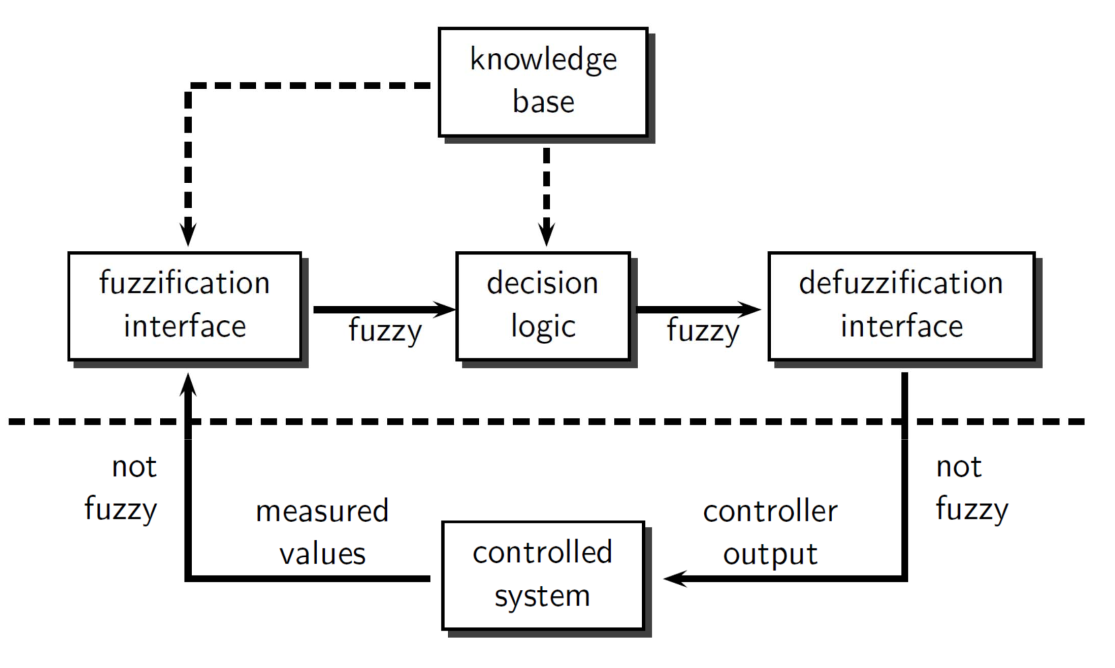
\includegraphics[scale=0.3]{img/fuzzycontroller.png}
\caption{Architettura di un fuzzy controller.}
\label{fig:30}
\end{figure}

Un'applicazione di particolare successo di queste idee sono i così detti \emph{fuzzy controller}. Il concetto che sta sotto al fuzzy control è quello di definire transizioni non-lineari tra i diversi stati del sistema senza specificare un insieme di equazioni differenziali per ogni variabile. Questo permette di modellare sistemi complessi le cui dinamiche possono sfuggire ad un'analisi matematicamente precisa. Lo schema di base di un fuzzy controller viene mostrato in Figura \ref{fig:30}. La (1) \emph{fuzzyfication interface} riceve i valori in input e si occupa di convertirli in un dominio adeguato (termini linguistici o fuzzy set). La (2) \emph{knowledge base} consiste di (a) dati che contengono informazioni riguardo intervalli, trasformazioni di dominio e a quali insiemi fuzzy corrisponderanno i termini linguistici, e (b) regole che contengono i controlli del tipo \emph{if-then}. La (3) \emph{decision logic} rappresenta l'unità processore, la quale si occupa di computare l'output in base all'input misurato e la knowledge base. Infine, la (4) \emph{defuzzification interface} si occupa di mappare i valori fuzzy usati nella computazione in valori booleani che sono inviati come segnali al controllo del sistema. 

\subsubsection{Defuzzification}

La mappatura dei segnali fuzzy interni al controller in segnali booleani utili a controllare il sistema può essere operata in svariati modi. In letteratura i più comuni sono:

\begin{enumerate}
\item{Max Criterion Method (MCM)}
\item{Mean of Maxima (MOM)}
\item{Center of Gravity (COG)}
\end{enumerate}

Il MCM sceglie un valore arbitrario $y \in Y$ per cui si raggiunge il massimo valore di appartenenza. Ha l'indubbio vantaggio di essere applicabile a qualsiasi fuzzy set e a domini $Y$ arbitrari. Può, tuttavia, essere difficile individuare l'elemento per cui la funzione di appartenenza viene massimizzata. Inoltre, la scelta di valori casuali rende il comportamento del controller non deterministico e questo può portare ad azioni discontinue.
Il MOM  prende $Y$ come intervallo e ne calcola l'insieme $Y_{MAX}$ tale che l'output in quei punti è massimo (l'insieme deve essere non vuoto e misurabile). Il valore di output sarà calcolato come la media su $Y_{MAX}$. Come nel caso precedente questa tecnica può portare ad azioni discontinue. 
Il COG, come il MOM, preso $Y$ come un intervallo restituisce in output il centro dell'area. Solitamente ha un comportamento regolare, anche se la computazione è onerosa e può condurre a risultati controintuitivi. 


\subsubsection{Mamdani controller}

Il primo modello di fuzzy controller è il così detto \emph{Mamdani controller}, sviluppato nel 1975 da Mamdani e Assilian. Questo controller è basato su una serie di regole del tipo "if $X$ is $M_n$, then $Y$ is $N_m$" dove $M_n$ e $N_m$ sono intervalli che rappresentano termini linguistici. Sebbene le regole siano della forma \emph{if-then}, non devono essere interpretate come implicazioni logiche, quanto definizione parziali di una funzione. Collettivamente le regole possono essere rappresentate nello spazio come l'unione $S$ dei vari intervalli:
$$
S = \cup M_i \times N_i
$$
Le regole possono assumere come valori intervalli \emph{crisp} come in Figura \ref{fig:31} (a), oppure valori fuzzy come in Figura \ref{fig:31} (b). In ogni caso, dato un input $x_0$ l'ouput verrà calcolato come la composta del singoletto di $x_0$ e l'unione degli intervalli $S$ (in simboli, $\{x_0\} \circ S$) come in Figura \ref{fig:32}. Questo output sarà un fuzzy set che rappresenta solo una vaga o imprecisa descrizione dell'output desiderato. Per determinare il vero valore di output, l'output preliminare dovrà essere defuzzificato. Nel caso del Mamdani controller si utilizza il metodo COG, che permette di trovare un compromesso rispetto ai singoli output delle regole.
 
 
\begin{figure}

\begin{subfigure}{0.5\textwidth}
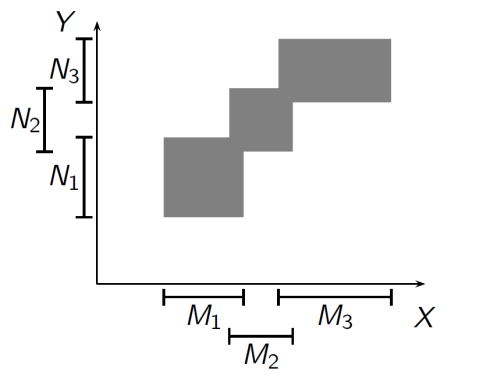
\includegraphics[width=0.9\linewidth, height=4cm]{img/rulesfuzzy.png} 
\caption{Regole a valori crisp.}
\end{subfigure} %%
\begin{subfigure}{0.5\textwidth}
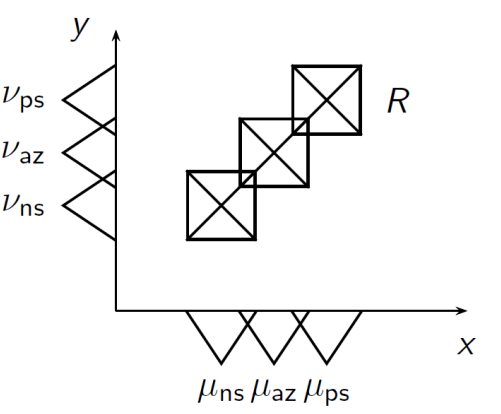
\includegraphics[width=0.9\linewidth, height=4cm]{img/fuzrule.png}
\caption{regole a valori fuzzy.}
\end{subfigure} 

\caption{Rappresentazione grafica di alcuni insiemi di regole.}
\label{fig:31}
\end{figure}


\begin{figure}
\centering
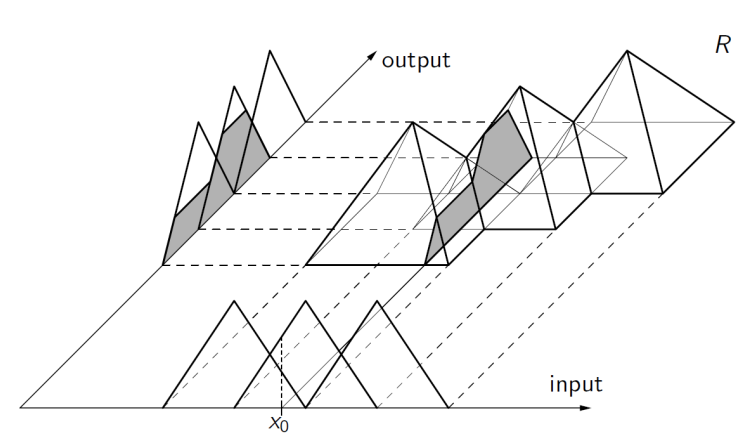
\includegraphics[scale=0.3]{img/outputrules.png}
\caption{Proiezione dell'ouput rispetto all'unione degli intervalli.}
\label{fig:32}
\end{figure}

\subsubsection{Takagi–Sugeno controller}

Questo controller può essere visto come una modifica e uno sviluppo del precedente. Nello stesso modo del Mamdani controller, i valori di input vengono descritti da fuzzy set. Tuttavia, il conseguente di una regola non sarà a sua volta un fuzzy set, ma una funzione che ha come argomenti le variabili di input (generalmente, una funzione lineare).

$$
R : \text{ if } x_1 \text{ is } \mu_1 \text{ and } \dots \text{ and } x_n \text{ is } \mu_n, \text{ then } y = f(x_1,\dots,x_n)
$$

 L'idea è che quella funzione è una buona funzione di controllo per la regione descritta dall'antecedente. Per mantenere la leggibilità del modello così prodotto, occorre evitare sovrapposizioni tra le varie regioni descritte nell'antecedente delle regole. Siccome l'ouput calcolato è già crisp, non occorre defuzzificarlo.
 
\subsubsection{Similarity-based reasoning}

Vi è un'ultima tipologia di controller che utilizza il concetto di relazione di somiglianza (l'analogo fuzzy delle relazioni di equivalenza).

\begin{definition}
Una funzione $E: X^2 \to [0,1]$ è definita \emph{relazione di somiglianza} rispetto ad una T-norma se e solo se soddisfa le seguenti condizioni:
\begin{enumerate}
\item{$E(x,x) = 1$}
\item{$E(x,y) = E(y,x)$}
\item{$\top (E(x,y),E(y,z)) = E(x,z)$}
\end{enumerate} 
\end{definition}

Questo genere di relazioni vengono utilizzate per tradurre l'informazione data dagli esperti in modo che le varie tuple coprano tutti i possibili comportamenti del sistema. Dalle classi di somiglianza possiamo poi estrarre regole in tutto uguali a quelle per il Mamdani controller.

\subsection{Fuzzy data analysis}

Ci sono due sensi in cui si parla di \emph{fuzzy data analysis}. Uno riguarda l'applicazione di tecniche di ragionamento fuzzy rispetto a dati crisp (si parlerà in questo caso di \emph{fuzzy clustering}). Un altro, invece, riguarda l'analisi di dati presentati sotto forma di fuzzy set (si parlerà in questo caso di \emph{random set} e \emph{random fuzzy variables}).

\subsubsection{Fuzzy clustering}


\begin{figure}
\centering
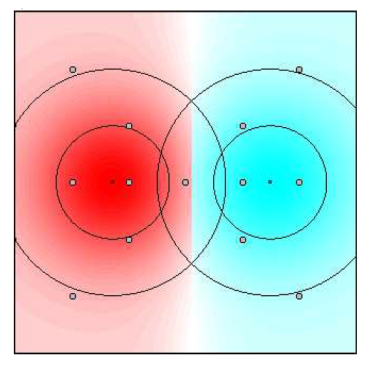
\includegraphics[scale=0.3]{img/symmetricdata.png}
\caption{Esempio di un dataset simmetrico.}
\label{fig:33}
\end{figure}

Il \emph{fuzzy clustering} è una procedura di apprendimento non supervisionato che permette di dividere il dataset in modo che a) oggetti nello stesso cluster siano quanto più possibili simili e b) oggetti in cluster diversi siano quanto più possibile dissimili. La relazione di somiglianza è misurata nei termini di una funzione distanza. Minore è la distanza, maggiore è la probabilità che due elementi appartengano allo stesso cluster. Nel caso dell'algoritmo \emph{hard c-means} si 1) sceglie un numero $c$ di cluster, 2) si distribuiscono in modo randomico i centri e 3) si procede all'assegnamento dei punti più vicini ai centri dei rispettivi cluster, poi 4) si passa ad aggiornare la posizione dei centri tramite il calcolo del centro di gravità. 5) Si ripete il processo fino a che la posizione si stabilizza. La partizione in cluster è ottimale quando la somma delle distanze tra i centri e gli elementi è minima. Un problema di questo approccio è che l'algoritmo può rimanere bloccato in minimi locali. Per ovviare a questo inconveniente solitamente si fanno varie iterazioni e se ne sceglie la migliore. Un diverso problema è quello che discende dal fatto che la partizione è crisp. Qualora, infatti, esista un elemento equidistante da due centri come in Figura \ref{fig:33}, l'assegnamento ad uno dei due cluster è puramente arbitrario e non rispecchia l'informazione fornita dai dati. Il \emph{fuzzy clustering} fornisce una soluzione a questo problema. Introducendo un concetto di appartenenza non binario ma continuo in $[0,1]$, offre la possibilità di esprimere l'appartenenza di un punto a più di un cluster. Il risultato sarà una partizione del dataset in fuzzy set. Possiamo rappresentare questa partizione attraverso una matrice che assegna ad ogni componente $u_{ij}$ il grado di appartenenza del punto $x_j$ al fuzzy set $\Gamma_i$, in simboli $u_{ij} = \mu_{\Gamma_i}(x_j)$. Esistono due tipi di fuzzy clustering: quello \emph{probabilistico} e quello \emph{possibilistico}. La differenza si gioca rispetto alle condizioni imposte alla funzione di appartenenza. Nel caso \emph{probabilistico} si avrà che:

\begin{enumerate}
\item{$\sum_{j=1}^{n} u_{ij} > 0, \quad \forall i \in \{1,\dots,c \} $}
\item{$\sum_{i=1}^{c} u_{ij} = 1, \quad \forall j \in \{1,\dots,n \} $}
\end{enumerate}

La prima condizione sta ad indicare che non possono esistere cluster vuoti, la seconda, invece, che l'appartenenza è esaurita dall'insieme dei fuzzy set che costituiscono la partizione. Nel caso \emph{possibilistico} si mantiene solo la prima assunzione e si lascia cadere la seconda. L'interpretazione possibilistica è da preferire quando si abbia a che fare con dati pieni di rumore o outlier.

\subsubsection{Problemi con il fuzzy clustering}

Come facciamo a sapere se la partizione in cluster operata dal nostro algoritmo rispecchia l'informazione implicita nei dati? Quale è l'ottimo numero di cluster per un dataset? Nel caso in cui abbiamo un numero limitato di dimensioni, possiamo rappresentare visivamente il dataset e avere un'intuizione di quanti centri avere e in quali posizioni collocarli. In generale, tuttavia, non è questo il caso. Per questo occorre definire una misura della qualità del clustering operato dall'algoritmo. Alcuni criteri da ricercare sono: una chiara separazione tra i cluster, minimo volume dei cluster, massimo numero di punti concentrati vicino al centro del cluster. In letteratura sono state proposte varie misure di questo tipo:

\begin{enumerate}
\item{\emph{Partition coefficient}: $PC = \frac{1}{n}\sum_{i=1}^{c} \sum_{j=1}^{n} u_{ij}^2$}
\item{\emph{Average partition density}: $APD = \frac{1}{c} \sum_{i=1}^c \frac{\sum_{j \in Y_i} u_{ij}}{\sqrt{|\sum_i|}}$}
\item{\emph{Partition entropy}: $PE = \sum_{i=1}^{c} \sum_{j=1}^{n} u_{ij} \log u_{ij}$}
\end{enumerate}

\subsubsection{Varianti}

La misura di distanza più intuitiva è quella euclidea, ma questa ha l'inconveniente di permettere solo cluster sferici. Alcune varianti sono state proposte per rilassarne i vincoli. Nell'algoritmo di \emph{Gustafson-Kessel} la distanza euclidea è sostituita con quella di \emph{Mahalanobis} definita rispetto ad un cluster $\Gamma_i$ come:
$$
d^2(x_j,C_j) = (x_j - c_i)^T \sum_i^{-1} (x_j - c_i)
$$
dove $\sum_i$ è la matrice covariante del cluster $i$. Questo algoritmo è preferito nel caso il clustering sia utilizzato per la generazione automatica di fuzzy rule per i controller. La dimensione dei vari cluster può variare a seconda del determinate della matrice (solitamente le dimensioni dei vari cluster sono le stesse e il determinante è uguale a 1). In generale l'algoritmo di Gustafson-Kessel estrae più informazioni dell'algoritmo standard, ma è anche più sensibile ad una corretta inizializzazione. Può essere utile per decidersi su una buona inizializzazione, procedere preliminarmente con alcune iterazioni dell'algoritmo standard. Data la presenza dell'inversione della matrice questo algoritmo è più costoso di quello standard e difficile da applicare a grossi dataset. Restringersi a cluster che risultano distribuiti lungo una retta parallela rispetto agli assi riduce il costo computazionale. Un altro approccio è quello di permettere cluster di forma non convessa.

\begin{figure}
\centering
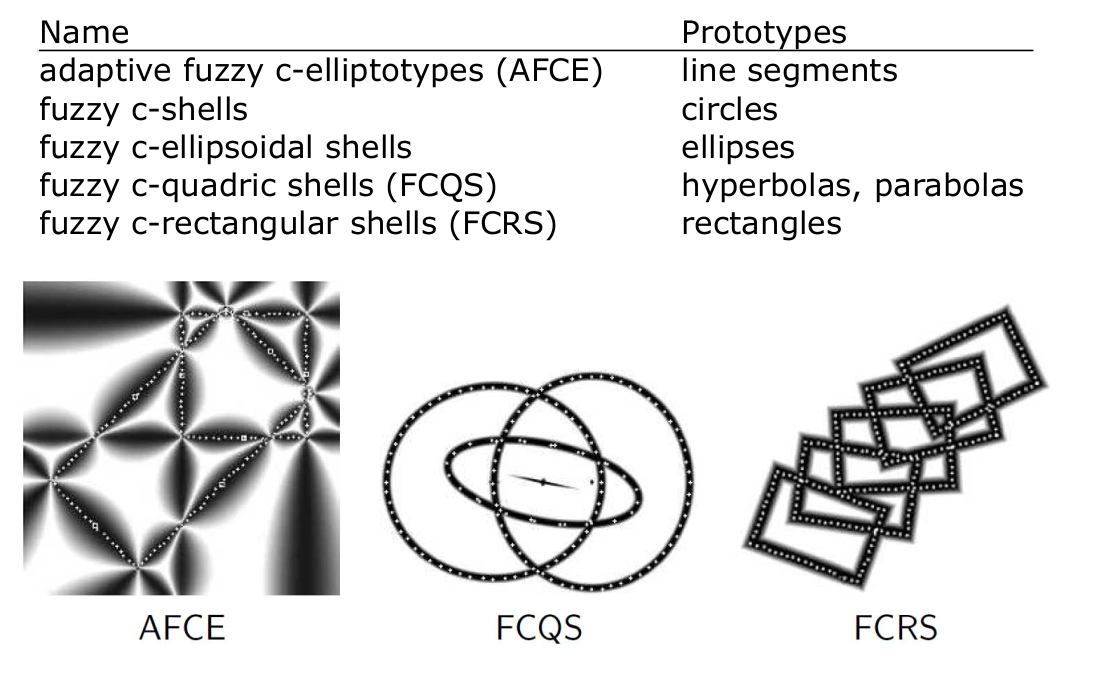
\includegraphics[scale=0.3]{img/shellcluster.png}
\caption{Alcuni esempi di shell clustering.}
\label{fig:34}
\end{figure}

Gli algoritmi di \emph{shell clustering} fanno proprio questo e sono particolarmente utili per il riconoscimento di immagini e la loro analisi. Nella Figura \ref{fig:34} si elencano alcuni esempi di questo genere di algoritmo. Un altro approccio presente in letteratura è quello del \emph{kernel-based clustering} che è utile qualora si abbia a che fare con dati non-vettoriali come sequenze, alberi o grafi. Questo metodo si basa su una mappa $\phi: \chi \to \mathbb{H}$, dove $\mathbb{H}$ è uno spazio di Hilbert e $\chi$ è lo spazio degli input. I dati così mappati non vengono utilizzati direttamente, ma solo attraverso il loro prodotto interno (la cui esistenza ci è garantita in quanto siamo in uno spazio di Hilbert). Si definisce per questo una funzione kernel $k$ tale che:
$$
k: \chi \times \chi \to \mathbb{R}, \forall x,x' \in \chi: <\phi(x),\phi(x')> = k(x,x')
$$
A differenza degli altri algoritmi di clustering non estrae dai dati dei prototipi per i singoli cluster, ma computa una relazione di somiglianza tra i vari input. I centri sono combinazioni lineari dei dati mappati in $\mathbb{H}$:

$$
c_i^{\phi} = \sum_{r=1}^n a_{ir} \phi(x_r)
$$

Alcuni svantaggi sono costiuiti dalla difficoltà nella scelta di una adeguata funzione kernel e dei parametri, e la mancanza di una esplicita rappresentazione dei singoli cluster. Un ultimo tipo di algoritmo è quello detto di \emph{noise clustering}. Questi algoritmi aggiungono un cluster $c$ che rappresenta tutti quei dati corrotti dal rumore o in altro modo non associabili a nessun altro cluster (outlier etc.). Il centro del cluster $c$ è scelto in modo da avere distanza costante da tutti i punti del dataset.

\subsubsection{Random set}

Se fin ad adesso abbiamo applicato tecniche fuzzy a dati crisp, ora vogliamo estendere queste tecniche in modo da comprendere descrizioni di dati fuzzy. Per fare questo occorre introdurre il concetto di \emph{random set}. Nel trattamento statistico standard dei dati la loro analisi è basata su variabili random, ovvero una funzione misurabile da uno spazio di probabilità ad un insieme $U$ (solitamente l'insieme $\mathbb{R}$). Un random set è una generalizzazione di questa idea, nel senso che il valore della funzione non sarà più un elemento dell'insieme $U$, bensì un suo sottoinsieme. Data una funzione $\Gamma: \Omega \to 2^U$, alcuni utili concetti da definire sono quello di \emph{limite superiore di probabilità} (in simboli $P^*(A)$) il quale indica la proporzione di elementi la cui immagine "tocca" un certo sottoinsieme di $U$:
$$
P^*(A) = P(\{ \omega \in \Omega | \Gamma (\omega) \cap A \neq \emptyset \})
$$
e quello di \emph{limite inferiore di probabilità} (in simboli $P_*(A)$) che indica la proporzione di elementi la cui immagine è interamente contenuta in un dato sottoinsieme di $U$:
$$
P_*(A) = P(\{ \omega \in \Omega | \Gamma (\omega) \subseteq A \text{ e } \Gamma(\omega) \neq \emptyset \})
$$
Attraverso questi strumenti possiamo analizzare dati descritti in modo fuzzy. Possiamo associare, infatti, ad ogni elemento della mappa una probabilità attesa $E(\Gamma)$ di modo che:
$$
E(\Gamma) = \{ E(X) | X(\omega) \in \Gamma(\omega) \text{ e la } X \text{ è una variabile randomica tale che } E(X), \forall \omega \in \Omega \}
$$
Possiamo generalizzare ancora il nostro approccio permettendo alla funzione $\Gamma$ di mappare gli input in un insieme fuzzy.

\subsection{Fuzzy neural network}

A differenza delle reti neurali, i fuzzy system hanno a che fare con il ragionamento ad alto livello, non si adattano al nuovo ambiente, usano informazioni linguistiche relative al dominio e non si basano sui dati. I \emph{fuzzy neural network} combinano la computazione parallela e le capacità di apprendimento delle reti neurali con la rappresentazione ad alto livello dei sistemi fuzzy. Questo permette di avere una interpretazione più perspicua dello stato interno della rete neurale durante la computazione. Vi sono due modalità in cui i sistemi fuzzy e le reti neurali possono collaborare.

\begin{itemize}
\item{modello \emph{cooperativo}: i due sistemi lavorano indipendentemente. La rete neurale genera certi parametri (offline) o li ottimizza (online) per il fuzzy controller.}
\item{modello \emph{ibrido}: i fuzzy set e le regole fuzzy sono mappate all'interno di una rete neurale. Le due strutture sono integrate e non si richiede l'overhead di comunicazione. Sia l'apprendimento offline che online sono disponibili.}
\end{itemize}

Nella modalità ibrida, i fuzzy set che appaiono negli antecedenti delle regole fuzzy, possono essere modellati sia come pesi delle connessioni tra neuroni, oppure come funzione di attivazione dei neuroni stessi. Nel primo caso, i neuroni del primo strato rappresentano la regola. Nel secondo, i neuroni del primo strato rappresentano l'insieme di input, mentre quelli del secondo la regola.

\subsubsection{Algoritmo}

Un insieme di regole fuzzy può essere tradotto in una rete neurale tramite la seguente procedura:

\begin{enumerate}
\item{Per ogni variabile di input $x_i$ si crea un neurone nel layer di input.}
\item{Per ogni variabile di output $y_i$ si crea un neurone nel layer di output.}
\item{Per ogni fuzzy set $\mu_i^j$ si crea un neurone nel primo layer hidden e lo si connette al neurone di input corrispondente a $x_i$.}
\item{Per ogni regola fuzzy $R_i$ si crea un neurone nel secondo layer hidden e si specifica una T-norma per calcolare l'antecedente della regola.}
\item{Si connette ogni neurone ai neuroni che rappresentano i fuzzy set degli antecedenti della loro regola corrispondente.}
\end{enumerate} 

A questo punto l'algoritmo diverge a seconda di quale tipo di controller si voglia utilizzare:

\begin{itemize}
\item{nel caso del Mamdani–Assilian controller, si connette ogni neurone "regola" al neurone di output corrispondente al dominio del conseguente nella regola fuzzy. Come peso della connessione si sceglie il fuzzy set del conseguente della regola fuzzy.}
\item{nel caso del Takagi–Sugeno–Kang controller, per ogni neurone "regola" si crea un gemello che computa la funzione di output della corrispondente regola fuzzy e gli si connettono tutti i neuroni di input.}
\end{itemize}

Il network così costruito può essere allenato grazie alla backpropagation.

\begin{figure}
\centering
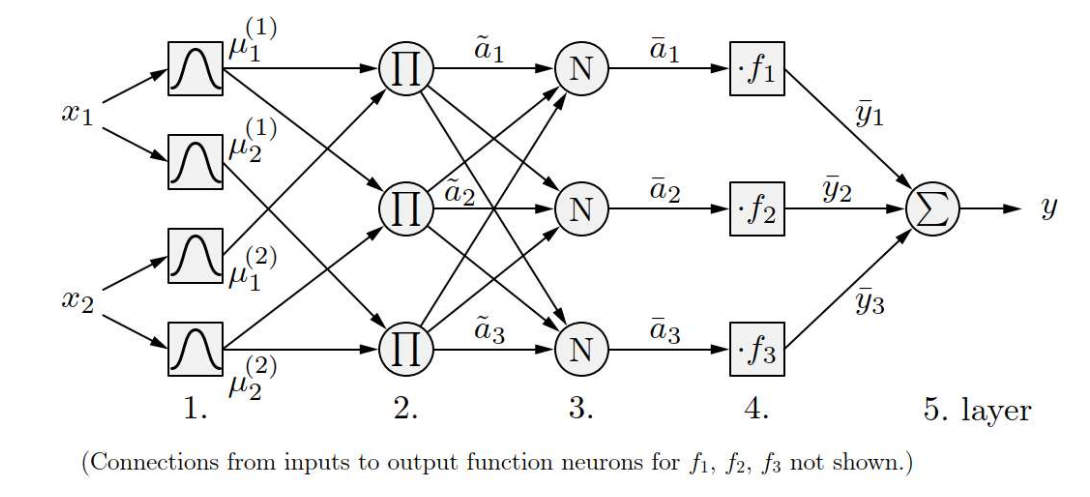
\includegraphics[scale=0.3]{img/fuzzyneural.png}
\caption{Adaptive Network-based Fuzzy Inference
Systems (ANFIS)}
\label{fig:35}
\end{figure}

\section{Algoritmi evolutivi}

\subsection{Introduzione}

Un \emph{problema di ottimizzazione} può essere descritto da una tripla $(\Omega,f,\prec)$ dove $\Omega$ è lo spazio di ricerca, $f$ è una funzione di valutazione della forma $f:\Omega \to \mathbb{R}$ e $\prec$ un preordine. L'insieme $H \subseteq \Omega$ tale che:

$$
H = \{ x \in \Omega | \forall x' \in \Omega: f(x) \succeq f(x') \}
$$

è definito l'insieme degli \emph{ottimi globali}. Dato un problema di questo genere la sua soluzione sta nel fornire un elemento che appartiene all'insieme $H$. In letteratura sono stati proposti vari metodi di soluzione per i problemi di ottimizzazione:
\begin{itemize}
\item{Soluzioni analitiche}
\item{Brute-forcing}
\item{Random search}
\item{Ricerca guidata}
\end{itemize}
Tutti questi metodi hanno delle criticità o sono applicabili solo ad alcuni tipi di funzione. Gli \emph{algoritmi evolutivi} rispondono a questo problema adottando una strategia innovativa. Tali algoritmi sono direttamente ispirati alla teoria della evoluzione biologica i cui principi fondamentali sono:
\begin{enumerate}
\item{Tratti vantaggiosi che sono risultato di mutazioni casuali tendono ad essere favoriti dalla selezione naturale}
\item{Gli individui che mostrano questi tratti vantaggiosi hanno migliori opportunità di procreare e moltiplicarsi}
\end{enumerate}

Gli elementi di un algoritmo evolutivo sono:

\begin{enumerate}
\item{una \emph{codifica} per i candidati: dipende molto dal problema e non esistono regole generali.}
\item{un metodo per creare una \emph{popolazione iniziale}: di solito si crea casualmente.}
\item{creare una \emph{funzione di fitness} per valutare i candidati: rappresenta l'ambiente e spesso è la stessa funzione da ottimizzare.}
\item{dei \emph{metodi di selezione} in relazione ai valori di fitness: si scelgono così gli individui che dovranno procreare nella successiva generazione.}
\item{un insieme di \emph{operatori genetici} che modifichino i cromosomi: i due più usati sono quello di a) \emph{mutazione}, che modifica in modo random i cromosomi e quello di b) \emph{crossover} che ricombina i cromosomi dei genitori per creare la prole.}
\item{alcuni parametri come \emph{dimensione della popolazione}, \emph{probabilità di mutazione}, etc.}
\item{una \emph{condizione di terminazione}: numero di generazioni, approssimazione all'ottimo, etc.}
\end{enumerate}

\subsection{Definizione formale}

Per ogni problema di ottimizzazione occorre separare lo spazio dei \emph{fenotipi} $\Omega$ (ovvero, come l'individuo appare) da quello dei \emph{genotipi} $\Gamma$ (ovvero, come l'individuo è rappresentato dalla codifica scelta). La funzione di fitness sarà definita sui fenotipi, dove, invece, gli operatori genetici agiranno sui genotipi. Per valutare i cambiamenti nel genotipo sarà necessario provvedere una funzione di \emph{decodifica} $dec: \Gamma \to \Omega$.

\begin{definition}
Ogni \emph{individuo} $A$ è rappresentato da un tupla $(A.G, A.S, A.F)$ contenente il genotipo ($A.G \in \Gamma$), informazioni e parametri addizionali $A.S \in Z$ e la valutazione dello stesso rispetto alla funzione di fitness $A.F = f(dec(A.G))$.
\end{definition}

\begin{definition}
L'operatore di \emph{mutazione} è definito come una mappa:
$$
Mut^{\xi} : \Gamma \times Z \to \Gamma \times Z
$$
dove $\xi$ è un numero randomicamente generato.
\end{definition}

\begin{definition}
L'operatore di \emph{ricombinazione} avente $r \geq 2$ genitori e $s \geq 1$ figli è definito come una mappa:
$$
Rek^\xi : (\Gamma \times Z)^r \to (\Gamma \times Z)^s
$$
dove $\xi$ è un numero randomicamente generato.
\end{definition}

\begin{definition}
L'operatore di \emph{selezione} ci permette di scegliere grazie ai valori di fitness tra una popolazione di $r$ individui un numero $s$ di individui che continueranno la specie. Sia $P = \{\ A_1, \dots, A_r \} $ la popolazione di individui allora l'operatore di selezione avrà la forma:
$$
Sel^\xi : (\Gamma \times Z \times \mathbb{R})^r \to (\Gamma \times Z \times \mathbb{R})^s
$$
$$
A_{i \quad 1 \leq i \leq r} \mapsto A_{IS^\xi (c_1,\dots,c_r)_k \quad 1 \leq k \leq s } 
$$
dove la selezione ha la forma:
$$
IS^\xi : \mathbb{R}^r \to \{ 1, \dots, r \}^s
$$
\end{definition}


\begin{figure}
\centering
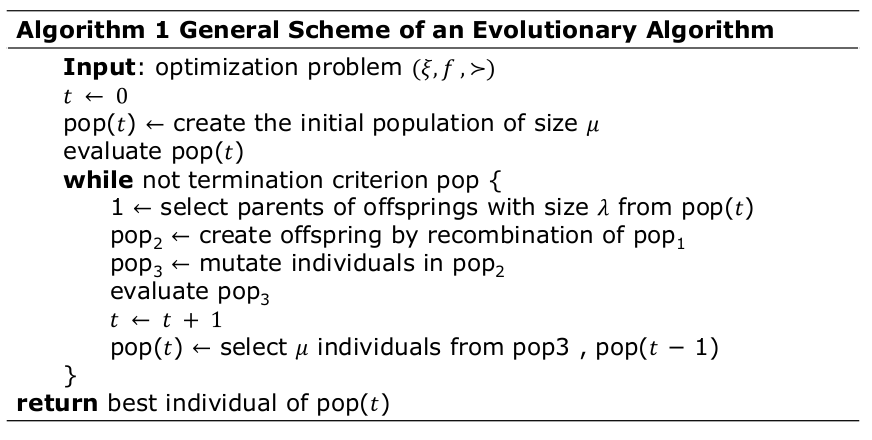
\includegraphics[scale=0.3]{img/evalg.png}
\caption{Pseudocodice di un generico algoritmo evolutivo}
\label{fig:36}
\end{figure}

Siamo, ora, pronti a dare una definizione formale di algoritmo evolutivo:

\begin{definition}
Un \emph{algoritmo evolutivo} su un problema di ottimizzazione $P$ è una tupla $(\Gamma, dec, Mut, Rek, IS_{genitori}, IS_{ambiente}, \mu, \lambda)$. Dove $\mu$ descrive il numero degli individui della generazione precedente e $\lambda$ descrive il numero di figli per generazione.
$$
Rek : (\Gamma \times Z)^k \to (\Gamma \times Z)^{k'}
$$
$$
IS_{genitori} : \mathbb{R}^\mu \to \{ 1, \dots, \mu \}^{\frac{k}{k'}\cdot \lambda} \quad \frac{k}{k'}\cdot \lambda \in \mathbb{N}
$$
$$
IS_{ambiente} : \mathbb{R}^{\mu + \lambda} \to \{ 1, \dots, \mu + \lambda \}^\mu
$$
\end{definition}

Vi è una distinzione che si può tracciare all'interno degli algoritmi evolutivi:

\begin{itemize}
\item{gli \emph{algoritmi genetici}: dove la codifica è una sequenza binaria}
\item{e gli \emph{algoritmi evolutivi} propriamente detti: dove la codifica dipende dal problema trattato e così gli operatori genetici.}
\end{itemize}

\subsection{Meta-euristiche}

Una \emph{meta-euristica} è un metodo algoritmico per trovare soluzioni approssimate di un problema di ottimizzazione combinatoria. Si definiscono sequenze astratte di passi che possono essere applicate a qualsiasi problema del genere. Ogni singolo passo deve poi essere declinato a seconda della specificità del problema. Il bisogno per un approccio meta-euristico nasce dal fatto che alcune classi di problemi non hanno una efficiente soluzione algoritmica. L'approssimazione che si otterrà rispetto alla soluzione ottima dipende dalla definizione del problema e dall'implementazione dei singoli passi del meta-algoritmo.

\subsubsection{Local search method}

Una meta-euristica è quella comunemente chiamata \emph{local search method} e costituisce un caso particolare di algoritmo evolutivo. Dato un problema di ottimizzazione $P$ e la funzione da ottimizzare $f$, questo metodo cerca i massimi globali \emph{localmente}, attorno cioè ai punti scelti durante la fase di inizializzazione. L'assunzione che si fa è che il valore della funzione in $x_1$ e $x_2$ differisce meno quanto più i due argomenti sono simili: $f$ non ha salti. 
La particolarità di questo approccio evolutivo è che la popolazione si limita ad un solo individuo. Questo ha alcune conseguenze, soprattutto rispetto agli operatori genetici: l'operatore di ricombinazione non è più necessario e ci si limita a quello di mutazione. Ad ogni passo si può decidere se continuare a mutare l'individuo o crearne uno diverso (per evitare minimi/massimi locali). L'idea è quella di utilizzare il \emph{gradient ascent/descent} per identificare un punto di massimo/minimo facendo un passo nella direzione del gradiente. L'ampiezza dei passi non deve essere troppo piccola perché in quel caso l'algoritmo convergerebbe troppo lentamente, nè troppo grande perché si rischiano oscillazioni. Per prevenire il fatto che si rimanga bloccati in minimi/massimi locali si eseguono varie iterazioni dell'algoritmo a partire da diversi punti. Se $f$ non risultasse differenziabile si cerca di determinare la direzione in cui $f$ cresce valutando punti casuali nell'intorno della posizione attuale (\emph{hill climbing}). Una generalizzazione dei precedenti approcci è ciò che in letteratura viene chiamato \emph{simulated annealing}. L'intuizione che ci sta dietro è che muoversi dal basso verso l'alto dovrebbe essere più probabile che il contrario. Per tanto, soluzioni migliori saranno sempre accettate, ma nel caso di soluzioni peggiori, queste potranno essere comunque accettate a seconda della loro "qualità". Si può applicare un valore soglia per decidere quanto una soluzione può essere peggiore rispetto alla precedente, oppure decidere un lower bound senza alcun confronto col valore precedente, etc.

\subsubsection{Tabu search}

L'algoritmo \emph{tabu search} può essere visto come una local search che, nel momento di creare un nuovo individuo, considera la storia delle passate generazioni. Si appronta una lista (FIFO) di \emph{tabu} che permette di evitare il ricorrere di candidati già testati. Ogni individuo è una soluzione completa. Le mutazioni non sono permesse. Se il nuovo candidato mostra "proprietà interessanti" può essere fatta una eccezione al tabu.

\subsubsection{Algoritmi memetici}

Un diverso approccio è quello degli \emph{algoritmi memetici}. Questi algoritmi uniscono i pregi dell'approccio \emph{population-based} (lento, ma che offre più informazioni) e quello \emph{local search} (veloce, ma suscettibile ai minimi locali). I "memes" sono elementi del comportamento che possono essere acquisiti individualmente. La procedura prevede per ogni individuo creato che lo si cerchi di ottimizzare e solo dopo che si consideri la popolazione nel suo intero. Questo permette spesso di accelerare il processo di ottimizzazione, ma le dinamiche "evolutive" sono limitate in modo critico: le mutazioni rischiano di bloccarsi frequentemente in minimi locali, la ricombinazione ha un raggio di azione limitato date le precondizioni che si impongono. 

\subsubsection{Evoluzione differenziale}

Un'altra strategia è quella dell'\emph{evoluzione differenziale}. Non abbiamo in questo caso un adattamento dell'ampiezza dei passi, ma si cerca di utilizzare le relazioni tra gli individui nella popolazione come base per calcolarla. Si introduce un particolare operatore genetico: \emph{DE-operator}. Questo operatore può essere visto come una combinazione dell'operatore di ricombinazione e quello di mutazione. Nella selezione, invece, un discendente può rimpiazzare i suoi antenati se e solo se ha un miglior valore di fitness. 

\subsubsection{Scatter search}

L'idea che sta alla base degli algoritmi \emph{scatter search} è quella di avere una popolazione e di operare una ricerca locale attorno agli individui. Dati i valori registrati da questa ricerca, si forza l'evoluzione a seconda della direzione del massimo registrato. Questo è un metodo puramente deterministico a differenza dei precedenti. La sua bontà dipende dalla copertura che riusciamo ad offrire dello spazio di ricerca. 

\subsubsection{Algoritmi culturali}

Oltre alle informazioni genetiche si possono considerare anche quelle "culturali" relative alle skill apprese dalle precedenti generazioni. Gli \emph{algoritmi culturali} cercano di trarre vantaggio da questa memoria generazionale di modo che gli individui vengano influenzati da quest'ultima. Esistono due tipi di sapere culturalmente rilevante:

\begin{itemize}
\item{\emph{Sapere situazionale}: relativo a generazioni tra loro prossime.}
\item{\emph{Sapere normativo}: sempre rilevante.}
\end{itemize}

\subsection{Elementi di algoritmi evolutivi}

\subsubsection{Codifica}

Le soluzioni al nostro problema devono essere codificate in modo che si possa esplorare lo spazio delle possibili soluzioni attraverso questa rappresentazione. Non esiste una ricetta generale: il problema della codifica è specifico per ogni problema. Tuttavia, esistono alcuni principi di massima da seguire:

\begin{enumerate}
\item{Rappresentare fenotipi simili con genotipi simili.}
\item{La funzione di fitness deve restituire valori simili per candidati simili.}
\item{Lo spazio $\Omega$ deve essere chiuso rispetto agli operatori genetici.}
\end{enumerate}

La 1) assicura che mutazioni di certi geni risultino in genotipi simili e che radicali cambiamenti permettano di evadere da minimi locali. La 2) previene che si scelga una codifica troppo o troppo poco epistatica \footnote{In biologia, un allele di un gene \emph{epistatico} sopprime gli effetti di tutti i possibili alleli di un altro gene. Nel contesto degli algoritmi evolutivi, sta indicare il grado di interazione tra geni del cromosoma.}. Se troppo, una singola mutazione potrebbe produrre casuali cambiamenti di fitness. Se troppo poco, l'efficienza dell'algoritmo ne risente. Le motivazioni per 3) sono abbastanza ovvie: se lo spazio di ricerca non è chiuso rispetto agli operatori genetici, un cromosoma modificato potrebbe non essere più decodificato e interpretato.  

\subsubsection{Fitness}

Gli individui migliori (quelli che hanno migliori valori di fitness) dovrebbero avere le migliori opportunità di riprodursi. Per fare questo occorre esercitare quella che in gergo viene chiamata \emph{selective pressure} nel processo di creazione delle nuove generazioni. Se la selective pressure è bassa, si parla di \emph{esplorazione dello spazio}: la deviazioni permessa rispetto agli individui è la più ampia possibile (tutto $\Omega$), vi sono buone possibilità di raggiungere il massimo globale. Se la selective pressure è alta, si parla di \emph{sfruttamento degli individui migliori}: si ricerca l'ottimo nelle vicinanze degli individui migliori, l'algoritmo converge velocemente, anche se col rischio di convergere ad un ottimo locale. Per poter scegliere la corretta selective pressure occorre una metrica per calcolarla. Alcune tra quelle utilizzate in letteratura sono:
\begin{itemize}
\item{\emph{selection intensity}: il differenziale tra prima e dopo che la selezione è avvenuta.}
\item{\emph{time to takeover}: il numero di generazioni prima che la popolazione converga.}
\end{itemize} 

Gli stessi metodi di selezione possono variare al variare della pressione evolutiva. Uno dei più usati è quello chiamato \emph{roulette-wheel selection}. Si computa il valore di fitness relativo di ogni individuo grazie alla seguente formula:

$$
f_{rel}(A_i) = \frac{A_i.F}{\sum_{j=1}^{|P|} A_j.F}
$$

La probabilità per un individuo di essere selezionato per la riproduzione sarà proporzionale al suo valore di fitness relativo. Alcuni svantaggi sono:

\begin{itemize}
\item{la computazione del valore di fitness relativo è costosa e difficilmente parallelizzabile.}
\item{gli individui con un alto valore di fitness potrebbero dominare la selezione (scomparsa delle biodiversità).}
\item{molto veloce a trovare ottimi locali, ma pessima esplorazione dello spazio.}
\end{itemize}

La stessa funzione di fitness può essere adattata per impedire una convergenza troppo rapida:

\begin{itemize}
\item{\emph{linear dynamical scaling}: riduciamo la rilevanza della funzione di fitness sottraendoci il minimo delle passate generazioni.}
\item{\emph{$\sigma$-scaling}: calcolata attraverso la formula $f_{\sigma}(A) = A.F - (\mu_f(t) - \beta \cdot \sigma_f(t))$, dove $\beta$ è un parametro positivo.}
\item{\emph{dipendente dal tempo}: il fattore temporale usato come esponente regola la selective pressure.}
\item{\emph{Boltzmann-selection}: determina la fitness relativa non direttamente, ma attraverso la funzione $g(x) = exp^{\frac{f(x)}{kT}}$. $T$ è una variabile che dipende dal tempo e $k$ è una costante di normalizzazione.}
\end{itemize}

\subsubsection{Selezione}

Vi sono varie strategie disponibili in letteratura per operare la selezione degli individui che costituiranno il pool genetico per la successiva generazione:

\begin{itemize}
\item{\emph{Roulette-wheel selection}: vedi sopra.}
\item{\emph{Rank-based selection}: si ordinano gli individui in ordine di fitness decrescente. A seconda della posizione si assegna ad ogni individuo un \emph{rank} e con esso si definisce la probabilità di essere selezionati. Si procede ad una selezione del tipo roulette-wheel. Questo modello riesce ad ovviare al problema della dominanza e regola la pressione di selezione. Lo svantaggio sta che occorre ordinare gli individui (complessità $O(n \log n)$).}
\item{\emph{Tournament selection}: si estraggono $k$ individui casualmente dalla popolazione. Tramite scontri individuali si decide il migliore, il quale riceverà la possibilità di riprodursi nella prossima generazione. Si riesce così ad evitare il problema della dominanza e si riesce a regolare la pressione di selezione grazie alla grandezza del torneo.}
\item{\emph{Elitismo}: i migliori individui della generazione precedente costituiscono la generazione successiva. L'elite così scelta non è immune dai cambiamenti apportati dagli operatori genetici. Il vantaggio è che la convergenza viene ottenuta rapidamente. Lo svantaggio è che c'è il rischio di rimanere bloccati in ottimi locali.}
\item{\emph{Crowding}: gli individui delle generazioni successive dovrebbero rimpiazzare gli individui più simili a loro. La densità locale in $\Omega$ non può crescere in modo indefinito. Questo permette una migliore esplorazione dello spazio.}
\end{itemize}

Di seguito listiamo alcune proprietà che possono caratterizzare i metodi di selezioni:

\begin{itemize}
\item{\emph{Static}: la probabilità di selezione rimane costante.}
\item{\emph{Dynamic}: la probabilità di selezione può variare.}
\item{\emph{Extinguishing}: può darsi il caso che la probabilità di selezione sia 0.}
\item{\emph{Preservative}: la probabilità di selezione è sempre maggiore di 0.}
\item{\emph{Pure-bred}: gli individui possono avere discendenti solo in una generazione.}
\item{\emph{Under-bred}: gli individui possono avere discendenti in più di una generazione.}
\item{\emph{Right}: tutti gli individui possono riprodursi.}
\item{\emph{Left}: i migliori individui possono non riprodursi.}
\item{\emph{Generational}: i genitori non possono mutare fin quando i loro discendenti non vengono creati.}
\item{\emph{On-the-fly}: i discendenti sostituiscono i genitori.}
\end{itemize}


\subsubsection{Operatori genetici}

Gli \emph{operatori genetici} sono applicati ad una frazione di individui scelti (popolazione intermedia). Vengono così generate mutazioni e ricombinazioni delle soluzioni già esistenti. Gli operatori genetici vengono classificati secondo la loro varietà in:

\begin{enumerate}
\item{One-parent operators}
\item{Two-parent operators}
\item{Multiple-parent operators}
\end{enumerate}

Nella prima classe possiamo trovare l'operatore di \emph{mutazione}, il quale introduce piccoli cambiamenti randomici nel genoma della soluzione a cui viene applicato. Risulta utile per introdurre biodiversità nel pool delle soluzioni e favorire l'esplorazione dello spazio di ricerca. Esistono vari metodi per operare una mutazione:

\begin{itemize}
\item{\emph{Standard mutation}: il valore di uno (o più) gene viene mutato.}
\item{\emph{Pair swap}: si scambia la posizione di due geni.}
\item{\emph{Shift}: si shifta a destra o sinistra un gruppo di geni.}
\item{\emph{Arbitrary permutation}: si permuta arbitrariamente un gruppo di geni.}
\item{\emph{Inversion}: si inverte l'ordine di apparizione di un gruppo di geni.}
\end{itemize}

Invece, l'operatore di gran lunga più importante tra quelli two-parent è quello di \emph{ricombinazione} o \emph{crossover}, il quale ha il compito, date due soluzioni, di creare attraverso una combinazione del loro codice genetico le soluzioni che costituiranno la generazione futura. Vi sono vari modi per operare questa ricombinazione:

\begin{itemize}
\item{\emph{One-point crossover}: si determina una posizione casuale nel cromosoma e si scambiano le due sequenze da un lato del taglio.}
\item{\emph{Two-point crossover}: si determinano due posizioni casuali nel cromosa e si scambia quell'intervallo di geni.}
\item{\emph{N-point crossover}: un generalizzazione dei precedenti. Si scambiano le aree incluse nei punti selezionati casualmente.}
\item{\emph{Uniform crossover}: per ogni gene si determina se scambiarlo o meno a seconda di un certo parametro di probabilità.}
\item{\emph{Shuffle crossover}: si procede inizialmente ad operare una permutazione randomica sui due cromosomi. Dopo si procede come nel one-point crossover e si conclude facendo l'unmixing.}
\item{\emph{Uniform order-based crossover}: simile allo uniform crossover, per ogni gene si decide se tenerlo o cambiarlo. Gli spazi sono riempiti nell'ordine di apparizione dei geni nell'altro cromosoma.}
\item{\emph{Edge-recombination crossover}: il cromosoma è rappresentato come un grafo. Ogni gene è un vertice che ha archi verso i suoi vicini. Gli archi dei due grafi vengono mischiati. Si preserva l'informazione relativa alla vicinanza.}
\end{itemize}

Un caso di multiple-parent operator è quello del \emph{diagonal crossover}. Simile al n-point crossover, ma vi partecipano più di due genitori. Dati $k$ genitori, si scelgono $k-1$ punti per il crossover e si procede shiftando diagonalmente le sequenze rispetto ai punti scelti. Aumentando il numero di genitori si ottiene un ottimo grado di esplorazione dello spazio. Alcune proprietà che possono caratterizzare gli operatori di crossover sono:

\begin{itemize}
\item{\emph{Positional bias}: quando la probabilità che due geni vengano ereditati assieme dallo stesso genitore dipende dalla posizione (relativa) dei due geni nel cromosoma. Deve essere evitato perché può rendere la disposizione dei geni cruciale per la riuscita dell'algoritmo.}
\item{\emph{Distributional bias}: quando la probabilità che un certo numero di geni siano scambiati tra i genitori non è la stessa per tutti i possibili numeri di geni. Deve essere evitato perché soluzioni parziali di differenti lunghezze hanno differenti probabilità di progredire alla generazione successiva. In generale, è meno problematico del positional bias.}
\end{itemize}

Per migliorare le performance delle mie soluzioni ho due strategie:

\begin{itemize}
\item{\emph{Interpolating recombination}: opero una fusione dei tratti dei due genitori in modo da creare nuovi discendenti. Si creano nuovi alleli e ne beneficiano particolarmente gli individui con migliore fitness. Per una esplorazione sufficientemente ampia di $\Omega$ nelle prime iterazioni occorre utilizzare una probabilità di mutazione molto alta.}
\item{\emph{Extrapolating recombination}: inferisco informazioni da una moltitudine di individui e creo nuovi alleli in accordo. L'influenza della diversità è difficilmente quantificabile.}
\end{itemize}

\subsubsection{Strategie di adattamento}

Un ultimo aspetto da considerare è quello delle \emph{strategie di adattamento} che rispondono a domande del tipo: dovremmo permettere che la mutazione introduca pesanti modifiche al fenotipo durante l'ottimizzazione? Per rispondere a questa ed altre domande occorre una metrica per misurare il miglioramento in fitness tra l'individuo e l'individuo mutato. 

\begin{definition}
Il \emph{miglioramento di fitness} di un individuo $A$ rispetto ad un individuo $B$ è definito come:
$$
imp(A,B) = |A.F - B.F|
$$ 
se $A.F > B.F$, altrimenti $0$.
\end{definition}

\begin{definition}
Il \emph{miglioramento relativo atteso} di un operatore $mut$ rispetto ad un individuo $A$ è definito come:
$$
imp_{rel} = E(imp(A,mut(A)))
$$ 
\end{definition}

Data questa metrica si può giudicare le performance di un particolare operatore genetico. La qualità di una mutazione non può, però, essere giudicata a prescindere dal livello attuale di fitness. In generale, più ci si avvicina all'ottimo più occorre usare operatori locali. Esistono varie strategie di adattamento possibili:

\begin{itemize}
\item{\emph{Predefined adaptation}: si definiscono i cambiamenti prima della run.}
\item{\emph{Adaptive adaptation}: si definisce una metrica per stabilire durante la run quali operatori adottare.}
\item{\emph{Self-adaptation}: si utilizzano informazioni aggiuntive sugli individui.}
\end{itemize}

\subsection{Swarm and population based optimization}

La \emph{swarm based optimization} e la \emph{population based optimization} sono due meta-euristiche usate in letteratura per sviluppare sistemi intelligenti multi-agente capaci di  comportamento cooperativo. Il concetto di \emph{swarm intelligence}, utilizzato per descrivere in natura il comportamento di alcune specie (api, formiche, etc), sta a significare la capacità della popolazione di cooperare per la soluzione di un problema. L'idea è che i singoli individui (unità con skill limitate) scambino tra loro informazioni e si coordinino senza l'aiuto di un controllo centrale. Esistono varie tipologie di euristiche di questo genere:

\begin{itemize}
\item{\emph{Particle swarm optimization}: ispirato al pattern biologico della ricerca del cibo in uccelli e pesci. Gli individui aggregano informazioni, creando un insieme di conoscenze comuni, al fine di presentare una sola soluzione. Ogni individuo è un candidato ad essere la soluzione.}
\item{\emph{Ant colony optimization}: ispirato al pattern biologico delle formiche che cercano una strada che le conduca al cibo. Gli individui scambiano informazioni modificando l'ambiente, in modo che gli altri possano seguire (o meno) le loro tracce. Ogni individuo è un candidato ad essere la soluzione.}
\end{itemize}

Dal lato della \emph{population based optimization} troviamo, invece, il così detto \emph{population-based incremental learning}. Gli individui vengono generati randomicamente in accordo ad una distribuzione di probabilità. In realtà, non abbiamo bisogno di conservare in memoria gli individui in modo esplicito, ma è sufficiente conservare le statistiche della popolazione. Come operatore di ricombinazione viene utilizzato lo uniform crossover. Per la selezione, si scelgono gli individui che migliorino le statistiche della popolazione. La mutazione, invece, si limita ad un semplice \emph{bit-flip}. La sua feature distintiva è che il \emph{learning rate}, ovvero il parametro che regola la possibilità di movimento degli individui nello spazio, cambia nel tempo e si riduce con il numero di iterazioni. Questo permette, inizialmente, grande mobilità, per stabilizzarsi poi quando un ottimo viene trovato. Alcuni problemi con questa strategia sono che 1) l'algoritmo può apprendere anche alcune dipendenze accidentali tra i cromosomi degli individui e 2) considerare i singoli bit in isolamento gli uni dagli altri. Un diverso genere di problema riguarda la rappresentazione statistica della popolazione: 3) la stessa statistica può rappresentare differenti popolazioni.

\subsection{Fondamenti teorici}

Per dimostrare la correttezza degli algoritmi evolutivi occorre considerare gli \emph{schemata}, ovvero cromosomi binari solo parzialmente specificati che codificano un particolare comportamento. Da qui, si partirà poi a studiare come il numero dei cromosomi che condividono lo schema si evolve rispetto alle generazioni. L'obiettivo è quello di fornire una stima stocastica che descriva come un algoritmo evolutivo esplora lo spazio di ricerca.

\begin{definition}
Uno \emph{schema} $h$ è una stringa di simboli di lunghezza $L$ sull'alfabeto $\{0,1,*\}$. Il carattere $*$ è una wildcard.
\end{definition}

\begin{definition}
Un cromosoma $c$ si dice che \emph{condivide} lo schema $h$ (in simboli, $c \triangleleft h$) se e solo se, escluse le posizioni in $h$ aventi il simbolo $*$, $h$ coincide con $c$.
\end{definition}

Per misurare gli effetti della selezione occorre calcolare la fitness dei cromosomi che condividono un certo schema. Di solito si sceglie come misura la \emph{media del fitness} relativa ai soli cromosomi che condividono lo schema. Gli individui che condivideranno lo schema nella generazione successiva saranno proporzionali a questa media. Per calcolare, invece, l'influenza dell'operatore di mutazione occorre misurare la probabilità che, avvenuta la mutazione, lo schema si preservi. Definiamo, quindi, il concetto di \emph{ordine} di uno schema.

\begin{definition}
L'\emph{ordine} di uno schema $h$ è il numero degli 1 e degli 0 in $h$, ovvero 
$$
ord(h) = \#1 + \#0
$$
\end{definition}

Possiamo, ora, calcolare la probabilità che un operatore di mutazione preservi lo schema $h$ grazie alla formula:

$$
(1 - p_m)^{ord(h)}
$$

Per concludere, la probabilità che il crossover (ci limiteremo al caso \emph{one-point}) preservi lo schema verrà misurato a seconda della \emph{lunghezza definitoria} dello schema stesso.

\begin{definition}
La \emph{lunghezza definitoria} di uno schema $h$ è la differenza tra l'ultima posizione in cui occorre un 1 o uno 0 in $h$ e la prima (in simboli, $dl(h)$).
\end{definition}

La probabilità che il punto di "taglio" divida il cromosoma in modo tale che lo schema finisca nel mezzo sarà calcolata come:

$$
\frac{dl(h)}{L-1}
$$

dove $L$ è la lunghezza del cromosoma. Definiamo, ora, alcuni concetti fondamentali per quello che segue.

\begin{definition}
Il \emph{valore atteso dei cromosomi che condividono lo schema} (in simboli, $N(h,t)$) è il numero di cromosomi che condividono lo schema durante la generazione $t$.
\end{definition}

\begin{definition}
Il \emph{valore atteso (dei cromosomi che condividono lo schema) dopo gli operatori genetici} sarà calcolato come:
$$
N(h,t + \Delta t_s + \Delta t_c + \Delta t_m) = N(h,t+1)
$$
dove i vari $\Delta$ dipenderanno dalle probabilità dei singoli operatori definite sopra.
\end{definition}

Un importante teorema, il così detto \emph{schema theorem}, ci dice che schemi con a) una fitness sopra la media, b) una lunghezza definitoria corta e c) con ordine basso, si riproducono in modo "quasi" esponenziale. Tuttavia, un altro importante teorema, il così detto \emph{no free lunch theorem}, ci dice che non esiste un algoritmo evolutivo che possa essere utilizzato efficientemente per ogni problema. La scelta della "giusta" codifica e dei "corretti" operatori genetici dipenderà dalla nostra conoscenza locale riguardo allo specifico problema.

\subsection{Programmazione genetica}


\begin{figure}
\centering
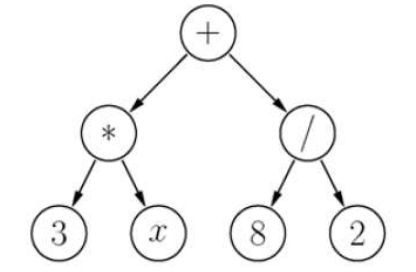
\includegraphics[scale=0.3]{img/parsetree.png}
\caption{Albero sintattico che rappresenta la funzione $3x + \frac{8}{2}$.}
\label{fig:37}
\end{figure}

La \emph{programmazione genetica} (in breve, GP) è una famiglia di algoritmi evolutivi che permettono la creazione automatica di programmi che possano risolvere problemi. Per fare questo occorre, innanzitutto, una codifica per rappresentare e manipolare un singolo programma. Solitamente si rappresentano programmi come \emph{alberi sintattici} dove i nodi interni sono le operazioni e le foglie variabili o costanti (vedi Figura \ref{fig:37}). L'insieme delle operazioni e dei simboli terminali varia da problema a problema. Se, per esempio, volessimo approssimare una funzione booleana sceglieremmo l'insieme di operazioni $F = \{and, or, not\}$ e come insieme di terminali $T = \{ x_0, \dots, x_n, 1, 0 \}$. GP può risolvere un problema efficacemente ed efficientemente solo se l'insieme di operazioni e di simboli terminali è \emph{completo} e \emph{sufficiente}. Il problema di trovare il più piccolo insieme completo e sufficiente per un dato problema è spesso NP-hard. Può essere utile rappresentare i cromosomi come espressioni del linguaggio $L = F \cup T$ per semplificare la computazione. 

\subsubsection{Inizializzazione}

Come nel caso degli algoritmi evolutivi visti in precedenza, occorre inizializzare una popolazione di individui (espressioni simboliche o alberi sintattici, in questo caso) creati in modo random. Data la complessità che esibiscono queste strutture, nel processo di creazione, bisogna considerare alcuni parametri quali l'\emph{altezza massima} degli alberi e il \emph{numero massimo di nodi}. Esistono vari sottoalgoritmi che si occupano dell'inizializzazione degli alberi sintattici:

\begin{enumerate}
\item{\emph{Grow}: la probabilità di scegliere un nodo interno o uno terminale è distribuita in modo uniforme a qualsiasi livello di profondità. Questo permette di creare alberi "sbilanciati".}
\item{\emph{Full}: i nodi terminali possono occorrere solo al livello dell'altezza massima dell'albero. Questo permette di creare alberi "bilanciati".}
\item{\emph{Ramp-half-and-half}: questo approccio mischia i primi due per avere più varianza nella forma esibita dagli alberi sintattici.}
\end{enumerate}

\subsubsection{Operatori genetici}

La popolazione così inizializzata difficilmente avrà un buon punteggio di fitness. Il processo evolutivo si occuperà di apportare cambiamenti alla popolazione attraverso operatori genetici. I tre più importanti sono:

\begin{itemize}
\item{\emph{Crossover}}
\item{\emph{Mutation}}
\item{\emph{Cloning} (duplicazione di un individuo)}
\end{itemize}

Nel caso del crossover, un approccio che si adotta spesso è quello dello scambio di due sottoespressioni: si scelgono due nodi interni e si scambiano tra i due alberi. Nel caso della mutazione, invece, si effettua sempre uno scambio di sottoalberi, ma con uno generato randomicamente.  

\subsubsection{Introni}

Durante il processo evolutivo gli individui tendono a sviluppare larghe porzioni di codice "inutile" ai fini della computazione. Un concetto simile ci viene dalla biologia: gli \emph{introni} sono porzioni di DNA che non codificano alcuna informazione a livello del fenotipo (per questo vengono talvolta chiamati \emph{junk-DNA}). Per evitare il verificarsi di questo fenomeno esistono alcune strategie:

\begin{itemize}
\item{\emph{Breeding recombination}: si generano molti figli usando parametri differenti, e si mantengono solo i migliori.}
\item{\emph{Intelligent recombination}: si scelgono in modo più selettivo i punti dove operare il crossover.}
\item{\emph{Continuos slight changes}: possiamo cambiare leggeramente la funzione di valutazione in modo che gli introni non siano più tali.}
\end{itemize}

\subsection{Strategie evolutive}

In una \emph{strategia evolutiva} cerchiamo non solo di ottimizzare i singoli individui, ma prendiamo in analisi l'intero processo evolutivo: riproduzione, mortalità, lunghezza media della vita degli individui, etc. Questi parametri sono suscettibili alle scelte che facciamo in materia di operatori genetici. Quello che facciamo è considerare un problema di ottimizzazione come una funzione $f: \mathbb{R}^n \to \mathbb{R}$ che vogliamo minimizzare. I cromosomi saranno rappresentati da array di reali (a differenza degli algoritmi visti in precedenza che utilizzavano per lo più rappresentazioni ad interi). Utilizziamo, poi, unicamente l'operatore di mutazione per muovere il vettore cromosoma all'interno dello spazio di ricerca aggiungendovi un vettore $r$ randomico ottenuto da una distribuzione normale. Il processo di selezione verrà applicato agli individui così mutati. Solo i migliori accederanno direttamente alla generazione successiva (elitismo). Per operare questa scelta vi sono due diversi approcci:

\begin{itemize}
\item{\emph{Plus-strategy}: la selezione lavora sull'insieme degli individui non mutati e degli individui mutati. }
\item{\emph{Comma-strategy}: si generano molti individui mutati e si sceglie tra loro chi costituirà la nuova generazione. I cromosomi non mutati vengono persi.}
\end{itemize}

Il vantaggio del primo approccio sta nel fatto che la fitness della popolazione non può che migliorare per la politica elitista che si adotta. Il problema è che si può rimanere bloccati in minimi locali. In questi casi può essere utile adottare la comma-strategy per creare diversità nella popolazione. Può anche essere opportuno adattare la varianza della mutazione durante il processo evolutivo. Se si permette una piccola varianza, allora avremo una esplorazione locale (\emph{exploitation}). Se, invece, si permette una ampia varianza, si avrà una ricerca globale (\emph{exploration}). Occorre scegliere un parametro $\sigma$ che ottimizzi la convergenza. Solitamente si utilizza la così detta $\frac{1}{5}$ \emph{success rule}: la varianza è appropriata quando $\frac{1}{5}$ degli individui mutati ha una miglior fitness rispetto a quelli della passata generazione. Si può anche avere un approccio più locale e conservare per ogni vettore cromosoma la sua varianza associata come un'informazione addizionale. I cromosomi con una "cattiva" varianza genereranno "cattivi" discendenti. I cromosomi (e le loro varianze) che hanno i peggiori valori di fitness non potranno accedere alle seguenti generazioni e si estingueranno. 

\subsection{Multi-criteria optimization}

Ci possono essere dei casi di problemi di ottimizzazione dove si hanno diversi obiettivi e vincoli, possibilmente in conflitto, ognuno rappresentato da una propria funzione di fitness $f_i : \Omega \to \mathbb{R}$. L'approccio più diretto è quello di combinare le varie funzioni in un'unica funzione di fitness aggregata:
$$
f(s) = \sum w_i \cdot f_i(s)
$$
Ognuna delle singole funzioni si vedrà assegnato un peso che rispecchierà la sua importanza relativa rispetto agli altri parametri. Il problema è quello di trovare una distribuzione dei pesi che rispetti i criteri di rilevanza. Se, inoltre, gli obiettivi sono tra loro in conflitto sarà ancora più difficile trovare una funzione che li aggreghi in modo opportuno. In generale, il teorema di impossibilità di Arrow previene la possibilità che esista una funzione di aggregazione che massimizzi tutte le singole funzioni. Una soluzione è quella di scegliere una soluzione solo se è un \emph{ottimo paretiano}.

\begin{definition}
Un elemento $s \in \Omega$ si dice \emph{ottimo paretiano} rispetto alle funzioni di valutazione $f_i$ con $i \in \{1, \dots, n\}$, se non c'è un elemento $s' \in \Omega$ tale che:
$$
\forall i, 1 \leq i \leq n: \quad f_i(s') \geq f_i(s)
$$ 
$$
\exists i, 1 \leq i \leq n: \quad f_i(s') > f_i(s)
$$
\end{definition}

Si potrà preferire una soluzione all'altra solo nel caso in cui nessuna funzione di valutazione peggiorerà nel caso si operi questa scelta. L'insieme delle soluzioni pareto-ottimali è detta \emph{frontiera paretiana}. Un vantaggio di questo approccio è che si evita il bisogno di aggregare le singole funzioni di valutazione e la ricerca è da operare solo uno volta. Possiamo utilizzare gli algoritmi evolutivi per trovare quante più soluzioni pareto-ottimali. Un approccio è quella di definire la funzione di fitness come la somma pesata delle singole funzioni di valutazione. Purtroppo questo favorisce soluzione che massimizzino una delle funzioni a discapito delle altre. Si può risolvere il problema individuando queste soluzioni "marginali" e scartandole in fase di selezione. Un secondo problema è quello della convergenza in un punto qualsiasi del fronte, si può rimediare applicando tecniche di \emph{power law sharing}, simili a quelle per evitare \emph{crowding}. Tali tecniche, tenendo conto delle zone già coperte del fronte, cercheranno di coprire punti inesplorati del fronte, in modo da garantire una copertura omogenea.

\subsection{Algoritmi evolutivi paralleli}

Rispetto alle altre metaeuristiche si è osservato che gli algoritmi evolutivi spesso portano a risultati ottimi, ma con il prezzo di un tempo di esecuzione molto lento.
È possibile parallelizzare alcune fasi del processo in modo da velocizzarlo o migliorarne il risultato. Osservando le varie fasi si nota che sono parallelizzabili:

\begin{itemize}
\item{la generazione iniziale, stando attendi ad eventuali duplicati, che comunque non costituiscono grossi problemi.}
\item{il calcolo del fitness degli individui, con l’accortezza di raccogliere i dati in un unico processore per calcolare il fitness relativo.}
\item{la selezione se costituita da eventi indipendenti, come ad esempio tournament selection, diventa più complesso gestire etilismo.}
\item{l’applicazione degli operatori genetici.}
\item{il controllo di raggiungimento del criterio di terminazione.}
\end{itemize}

Due architetture utilizzate in letteratura sono, rispettivamente:

\begin{itemize}
\item{\emph{Island model}: È possibile sfruttare la parallelizzazione considerando un modello ad isola. Ogni
isola avrà una popolazione, ed eseguirà il processo evolutivo. Si può introdurre migrazione degli individui da un isola all’altra in maniera random o definita da connessione tra le isole.}
\item{\emph{Cellular evolution}: I processori sono organizzati in una griglia. Ogni processore è responsabile di
un cromosoma.
Per la selezione ogni processore calcola il massimo dei vicini, gli operatori genetici sono applicabili solo tra vicini e la mutazione è gestita da ogni singolo
processore.}
\end{itemize}



\end{document} 
